\documentclass[twoside,11pt]{amsart}

\usepackage{amsmath,amsthm,amssymb, amstext,}
\usepackage{graphicx}
\usepackage{multirow}
\usepackage{url}
\usepackage{hyperref}
\usepackage{fancyhdr}
\usepackage{wrapfig}
\usepackage{caption}
\usepackage{lipsum}
%\fancypagestyle{plain}
\pagestyle{fancy}
%\fancyfoot{}
%\rfoot{NBHM}
%\rfoot{\thepage}
%\cfoot{anandice.ac.in/icrdet22/}
%\lfoot{ICRDET}
\usepackage{pdfpages}
%\usepackage{hangul}

\makeatletter
\renewcommand{\@evenhead}{\vbox{\thepage\hfil{\texttt{$\parallel$ 3${}^{\rm rd}$ ICRDET-2022, February 25-26, Anand-ICE, Jaipur, India $\parallel$}}\hrule}}
\renewcommand{\@oddhead}{\vbox{\hfill{\texttt{ $\parallel$ 3${}^{\rm rd}$ ICRDET-2022, February 25-26, Anand-ICE, Jaipur, India $\parallel$}}\hfill\thepage\hrule}}
\renewcommand{\@evenfoot}{\vbox{\hrule\begin{center}{\texttt{http://anandice.ac.in/icrdet22/index.html }}\end{center}}}
\renewcommand{\@oddfoot}{\vbox{\hrule\begin{center}{\texttt{http://anandice.ac.in/icrdet22/index.html }}\end{center}}}
%\renewcommand{\footrulewidth}{0.5pt}
\makeatother

\setlength{\oddsidemargin}{10pt} \setlength{\evensidemargin}{10pt}
\setlength{\textwidth}{5.8in}
\begin{document}
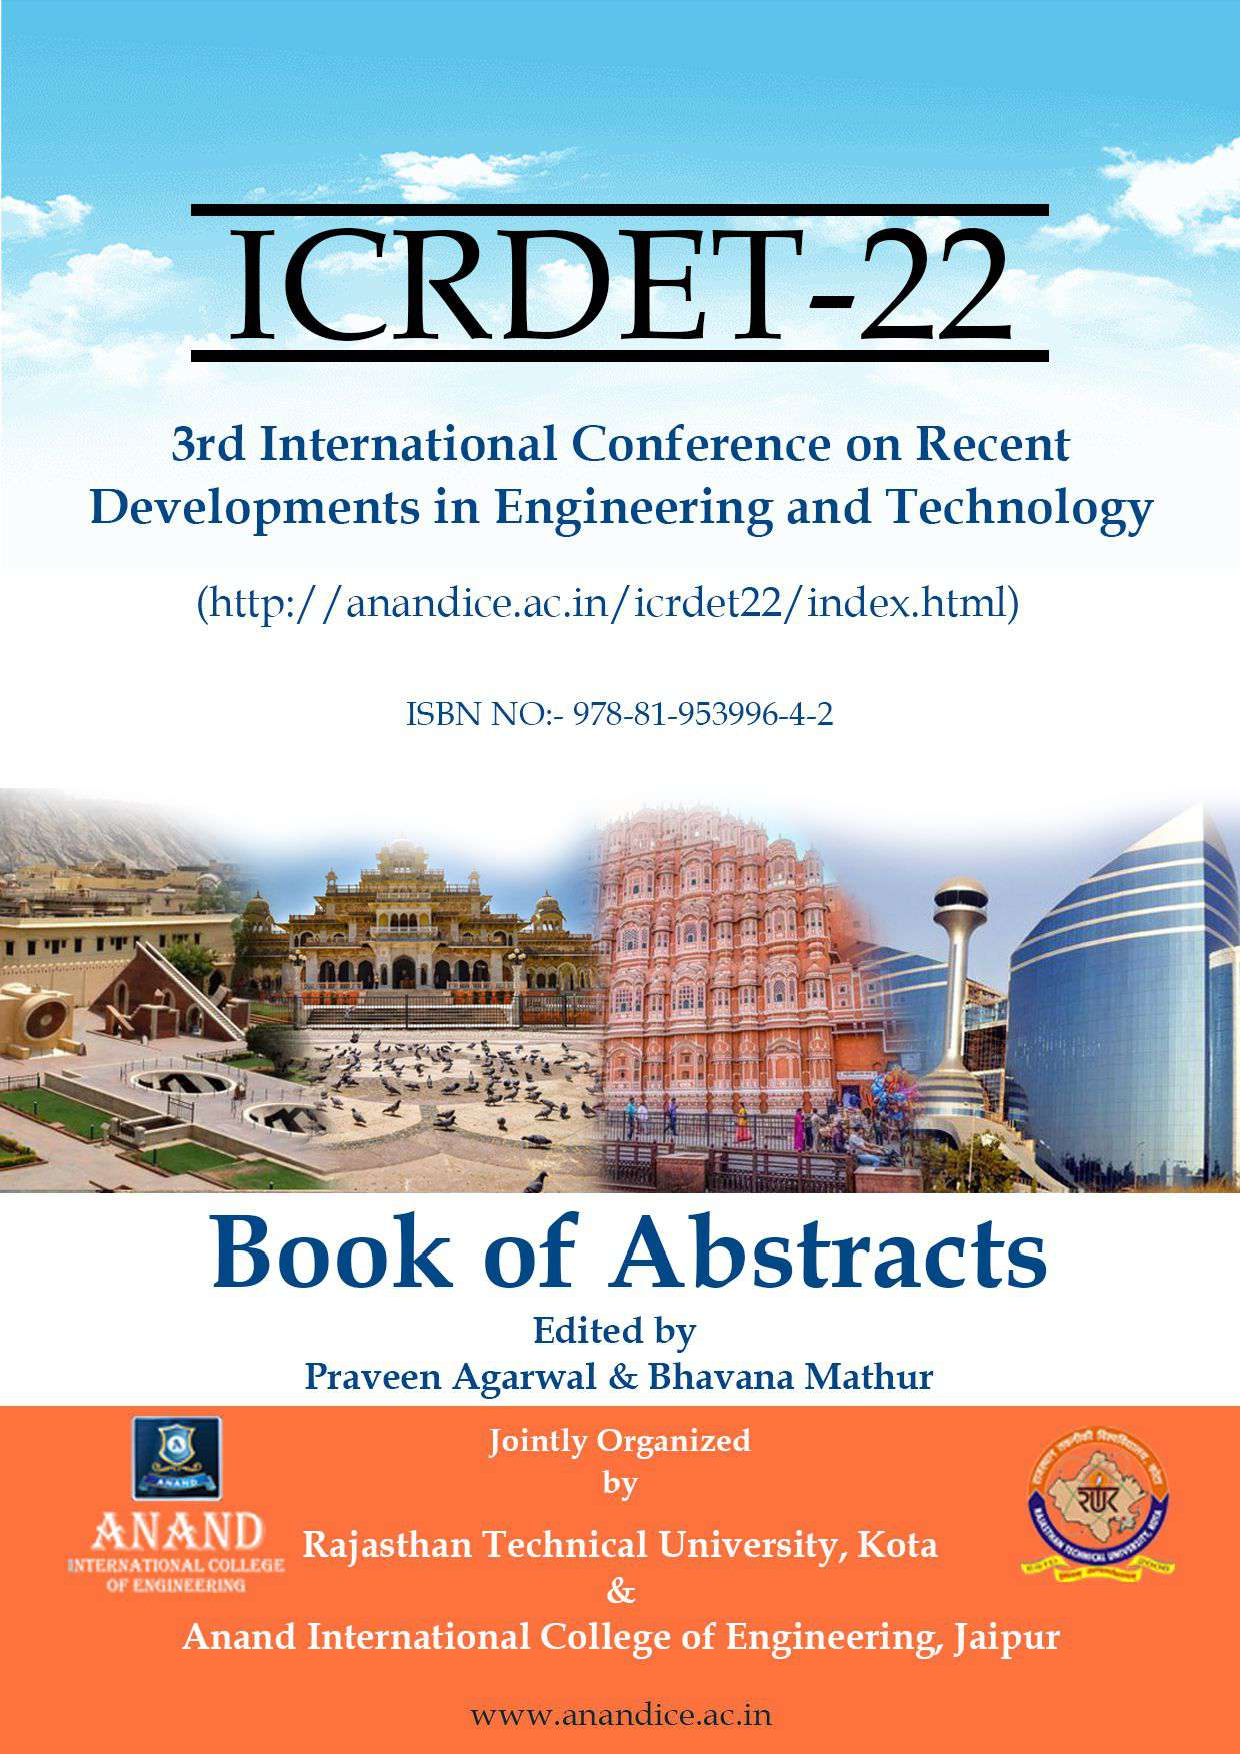
\includepdf[pages=1]{coverpage6}
\vspace*{25mm}

{\Huge
\begin{center}
The 3${}^{\rm rd}$(Hybrid) International Conference on Recent Development in Engineering \& Technology(ICRDET)

\end{center}
}
\vskip 105 mm


{\Large
\begin{center}
February 25 (Fri.) -- February 26 (Sat.), 2022

Anand International College of Engineering, Jaipur, India\\
(www.anandice.ac.in)
\end{center}
}


\thispagestyle{empty}

\newpage

\noindent
{\Large \bf International Advisory Board : }
\\
\begin{itemize}
\item Prof. Arni S.R. Srinivasa Rao(Augusta University, Augusta, USA)
\item Prof. Valentina E. Balas(Aurel Vlaicu University of Arad, ROMANIA)
\item Prof. Dumitru Baleanu(University Ankara, TURKEY)
\item Prof. Xiao-Zhi Gao(University of Eastern Finland, FINLAND)
\item Prof. Carlo Cattani(University of Tuscia, ITALY)
\item Prof. Yogendra Kumar Mishra(SDU NanoSYD, DENMARK)
\item Prof. Samad Noeiaghdam(Irkutsk National Research Technical University, Irkutsk, RUSSIA)
\item Prof. Ruzana Pskhu(Peoples’ Friendship University of Russia (RUDN-University), RUSSIA)
\item Prof. Xiao-Jun Yang(China University of Mining and Technology, Xuzhou, CHINA)
\item Prof. Tunde Joseph Taiwo(United Arab Emirates University, UAE)
\item Prof. Grienggrai Rajchakit(Maejo University, THAILAND)
\item Prof. Carla M. A. Pinto(Polytechnic of Porto, PORTUGAL)
\item Prof. Shams Forruque Ahmed(Asian University for women, Chittagong, BANGLADESH)
\item Prof. Jochen Merker(HTWK Leipzig University of Applied Sciences, GERMANY)
\item Prof. Shaher Momani(Ajman University, UAE)
\item Prof. Mehmet Yavuz(Necmettin Erbakan University, TURKEY)
\item Prof. Mohamed Abdel-Latif Ramadan(Menoufia University, EGYPT)
\item Prof. Nehad Ali Shah(Sejong University, KOREA)
\item Prof. Wen-Feng Wang(Shanghai Institute of Technology, CHINA)
\item Prof. Yeliz Karaca(University of Massachusetts, UMass Medical School, USA)


\end{itemize}

\newpage
\vskip 10mm
{\Large \bf National Advisory Board : }
\\
\begin{itemize}
\item Prof. Amit Kumar Verma(Indian Institute of Technology, Patna, INDIA)
\item Prof. Mani Mehra(IIT, Delhi, INDIA)
\item Prof. Rajesh Kumar(MNIT, Jaipur, INDIA)
\item Prof. Bhaskar Roy(Genpact, INDIA)
\item Prof. Santanu Saha Ray(National Institute of Technology, Rourkela, INDIA)
\item Prof. Jyotindra Prajapati(Sardar Patel University, Gujarat, INDIA)
\item Prof. Dhananjay Gopal(Guru Ghasidas Vishwavidyalaya (A Central University), Chhattisgarh, INDIA)
\item Prof. Manish Bhargava(NIT, Agartala, INDIA)
\item Prof. Dilip Kumar Sharma(MNIT, Jaipur, INDIA)
\item Prof. Shilpi Jain(PCE, Jaipur, INDIA)
\item Prof. Jankiballabh Sharma(RTU, Kota, INDIA)
\item Prof. Anita Tomar(Sri Dev Suman Uttarakhand University, Uttarakhand, INDIA)
\item Prof. Ram Singh(BGSB University, J\&K, INDIA)
\item Prof. M M Sharma(MNIT, Jaipur, INDIA)
\item Prof. Gunjan Saxena(Dy. Director General, Department of Telecom, Rajasthan, INDIA)
\end{itemize}
\noindent
\\
{\Large \bf Organizing Committee  : }
\\
\\
\\
\noindent
{\Large \bf Chief-Patron: }
\vskip 5mm
\begin{itemize}
\item \textbf{Prof. R. A. Gupta}(Honorable Vice Chancellor RTU, Kota, INDIA)
\end{itemize}
\vskip 5mm
\noindent
{\Large \bf Patrons: }
\vskip 5mm
\begin{itemize}
\item \textbf{Mr. Manoj Mittal}( Chairman, Anand-ICE, Jaipur,INDIA)
\item  \textbf{Ms. Monika Mittal}( Vice-Chairperson, Anand-ICE, Jaipur,INDIA)
\item \textbf{ Prof. Vijay Kr. Sharma}( Principal, Anand-ICE, Jaipur,INDIA)
\item \textbf{Prof. Praveen Agarwal}( Vice-Principal, Anand-ICE, Jaipur,INDIA)
\end{itemize}

%\begin{flushleft}
%{\bf Mr. Manoj Mittal} \hfill Chairman, Anand-ICE, Jaipur\\
%{\bf Ms. Monika Mittal}\hfill Vice-Chairperson, Anand-ICE, Jaipur\\
%{\bf Prof. Vijay Kr. Sharma}\hfill Principal, Anand-ICE, Jaipur\\
%{\bf Prof. Praveen Agarwal}\hfill Vice-Principal, Anand-ICE, Jaipur
%\end{flushleft}


%\begin{minipage}[l]{0.35\linewidth}
%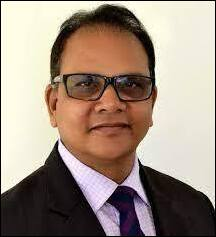
\includegraphics[height=8\baselineskip]{RA}
%\end{minipage}
%\hfill
%\begin{minipage}[r]{0.65\linewidth}
%\textbf{Prof. R. A. Gupta}\\
%Honorable Vice Chancellor\\
%%RTU, Kota, India
%\end{minipage}


%\begin{flushleft}
%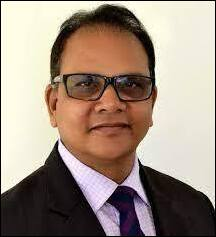
\includegraphics[width=3.5cm, height=3.5cm, keepaspectratio=false]{RA.jpg}
%\end{flushleft}
%\textbf{Prof. R. A. Gupta}\\
%Honorable Vice Chancellor\\
% RTU, Kota, India
%\newpage
%\noindent
%\\
%\\
%{\Large \bf Patron: }
%\\
%\\
%\begin{minipage}[l]{0.35\linewidth}
%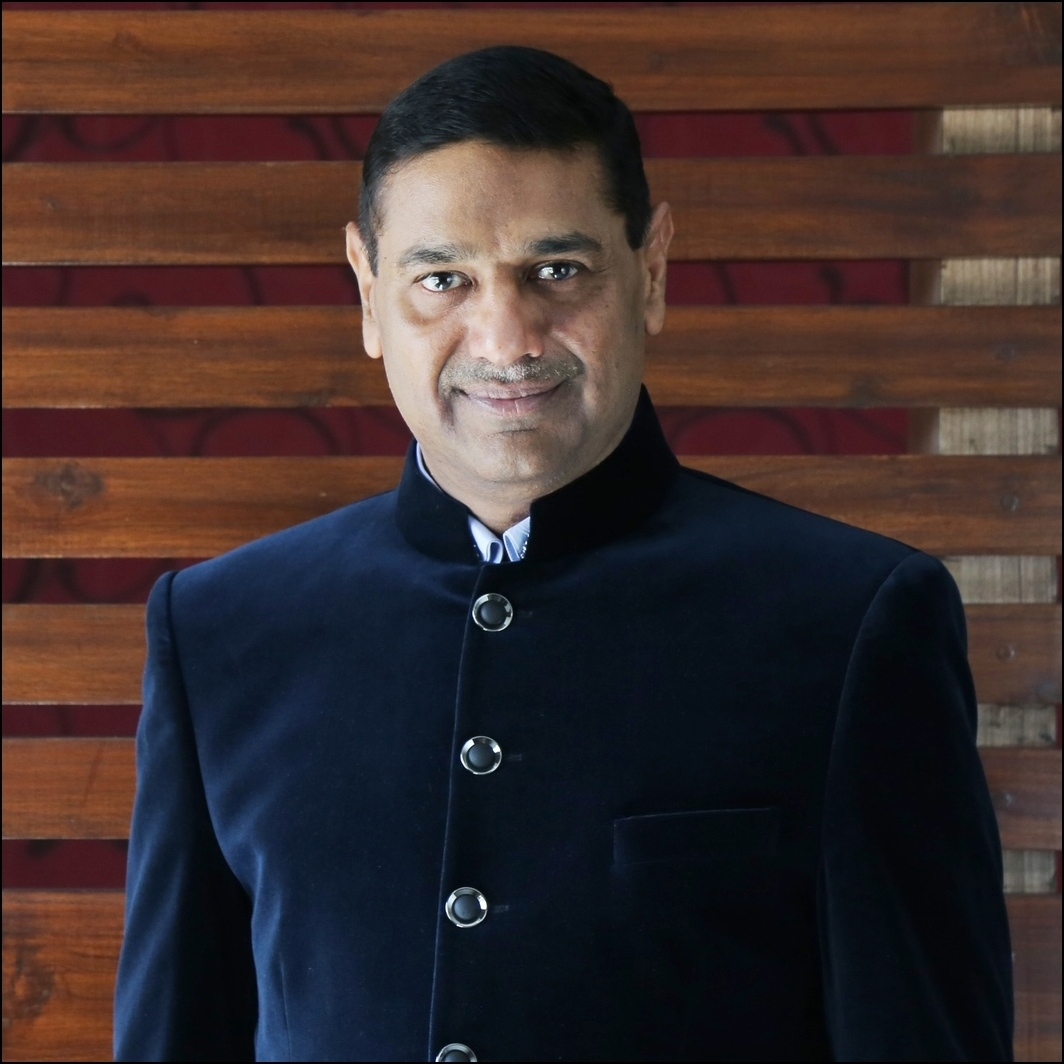
\includegraphics[height=8\baselineskip]{MM}
%\end{minipage}
%\hfill
%\begin{minipage}[r]{0.65\linewidth}
%\textbf{Mr. Manoj Mittal}\\
%Chairman, Anand-ICE\\
%Jaipur, INDIA
%\end{minipage}
%\\
%\\
%\\
%\\
%\begin{minipage}[l]{0.35\linewidth}
%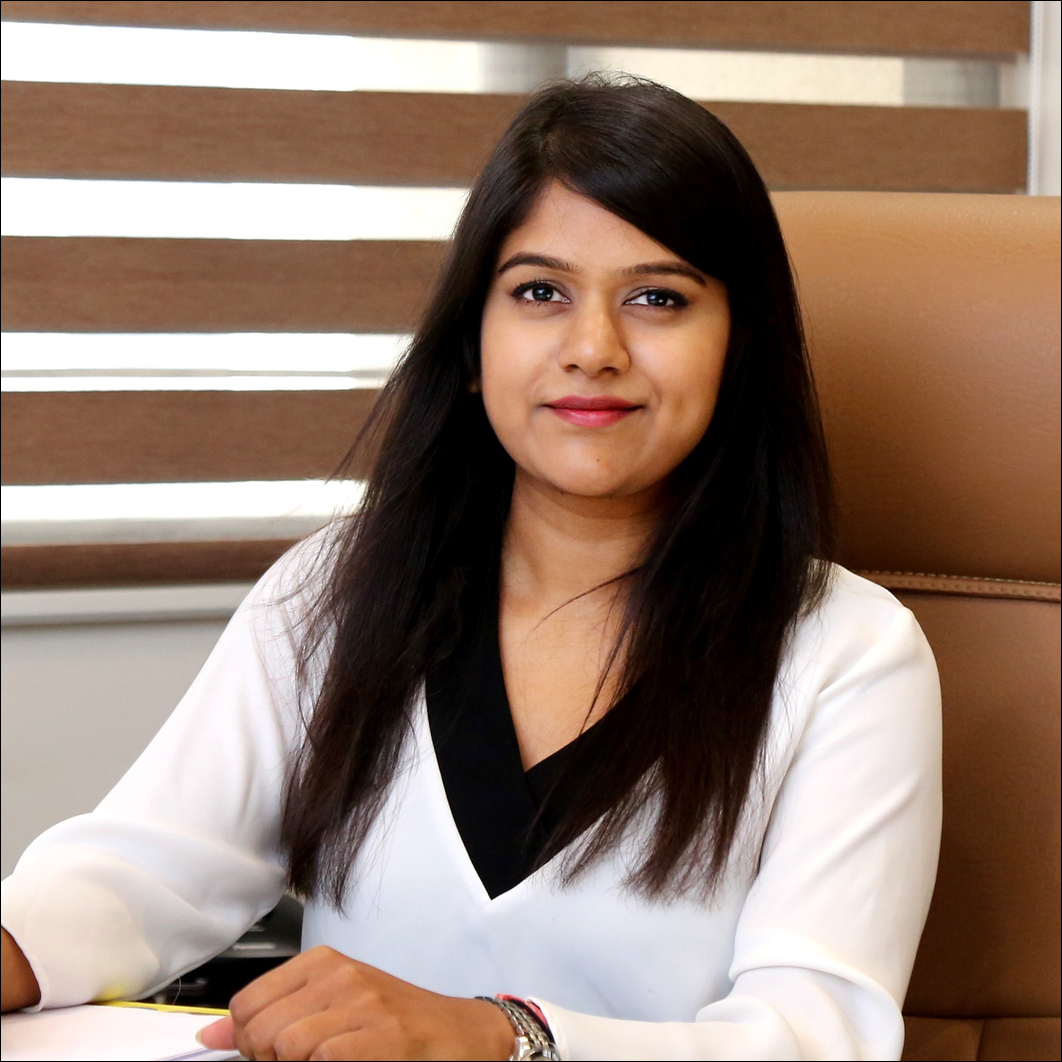
\includegraphics[height=8\baselineskip]{VC}
%\end{minipage}
%\hfill
%\begin{minipage}[r]{0.65\linewidth}
%\textbf{Ms. Monika Mittal}\\
%Vice Chairperson, Anand-ICE\\
%Jaipur, INDIA
%\end{minipage}
%\\
%\\
%\\
%\\
%\begin{minipage}[l]{0.35\linewidth}
%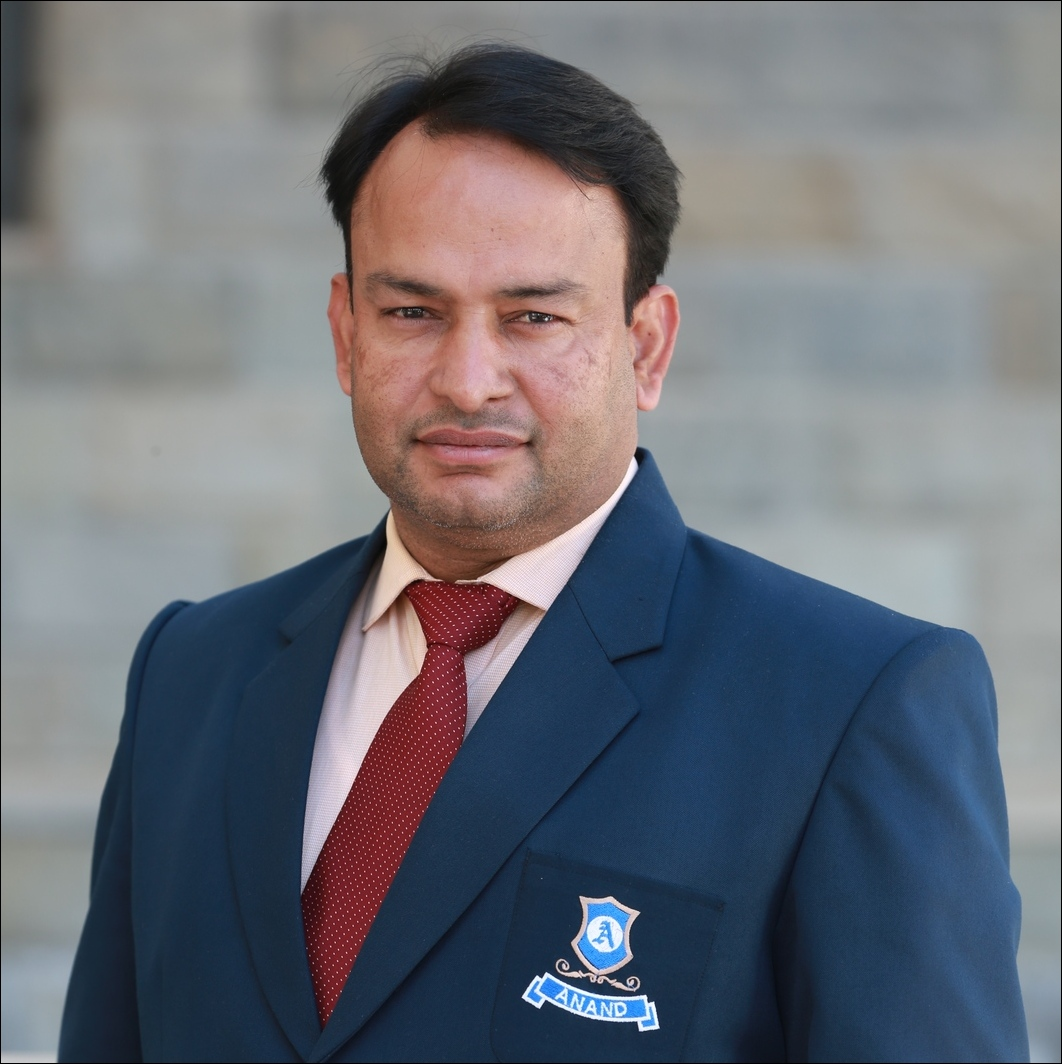
\includegraphics[height=8\baselineskip]{PP}
%\end{minipage}
%\hfill
%\begin{minipage}[r]{0.65\linewidth}
%\textbf{Prof. Vijay Kumar Sharma}\\
%Principal, Anand-ICE\\
%Jaipur, INDIA
%\end{minipage}
%\\
%\\
%\\
%\\
%\begin{minipage}[l]{0.35\linewidth}
%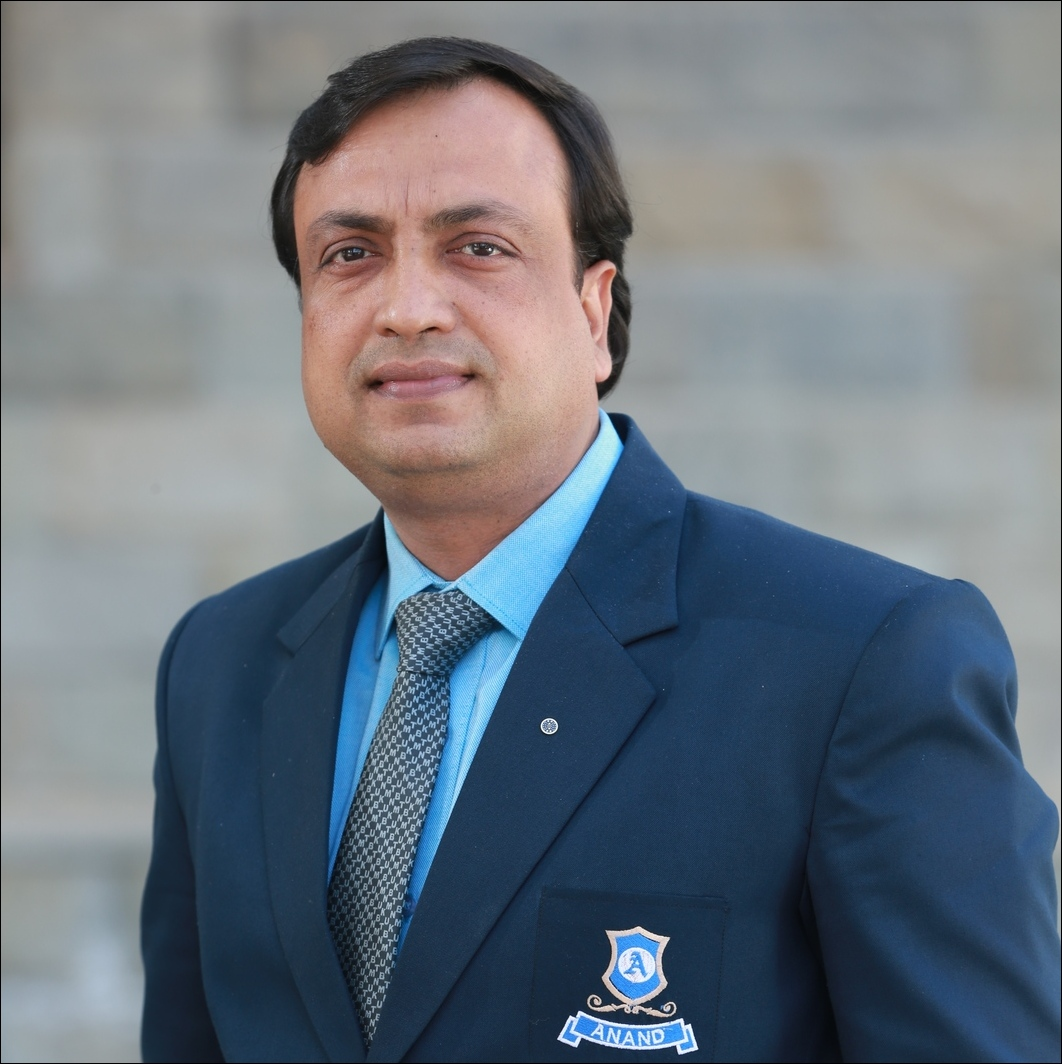
\includegraphics[height=8\baselineskip]{VP}
%\end{minipage}
%\hfill
%\begin{minipage}[r]{0.65\linewidth}
%\textbf{Prof. Praveen Agarwal}\\
%Vice Principal, Anand-ICE\\
%Jaipur, INDIA
%\end{minipage}
\newpage
{\Large \bf General Chairs :}
\\
\begin{itemize}
\item \textbf{Prof. Praveen Agarwal}(Anand-ICE, Jaipur, INDIA)
\item\textbf{Prof. Deepak Bhatia}(RTU, Kota, INDIA)
\end{itemize}
\noindent
\\
\\
{\Large \bf Organizing Chairs :}
\\
\begin{itemize}
\item \textbf{Prof. Bhavana Mathur}(Anand-ICE, Jaipur, INDIA)
\item\textbf{Prof. Harish Sharma}(RTU, Kota, INDIA)
\end{itemize}
\noindent
\\
\\
{\Large \bf Publicity Chairs :}
\\
\begin{itemize}
\item \textbf{Dr. Pushpendra Sharma}(JK Laxmipat University, Jaipur, INDIA)
\item\textbf{Prof. Anil Dhawan}(Anand-ICE, Jaipur,INDIA)
\item \textbf{Er. Pramil Sinha}(Anand-ICE, Jaipur, INDIA)
\item\textbf{Er. Neeraj Manglani}(Anand-ICE, Jaipur, INDIA)
\item \textbf{Er. Anubhav Saxena}(Anand-ICE, Jaipur, INDIA)
\item\textbf{Er. Shiv Kumar S}(Anand-ICE, Jaipur, INDIA)
\item\textbf{Er. Vivek Bhojak}(Anand-ICE, Jaipur, INDIA)
\end{itemize}
\noindent
\\
\\
{\Large \bf Website Development:}
\\
\begin{itemize}
\item \textbf{ Anubhav Saxena}(Anand-ICE, Jaipur, INDIA)
\item\textbf{ Shiv Kumar Sharma}(Anand-ICE, Jaipur, INDIA)
\end{itemize}
\noindent
\\
\\
{\Large \bf Promotion:}
\\
\begin{itemize}
\item \textbf{ Sanjog Arora}(Anand-ICE, Jaipur, INDIA)
\item\textbf{Rahul Goyal}(Anand-ICE, Jaipur, INDIA)
\end{itemize}
\noindent
\\
\\
{\Large \bf Registration Committee : }
\\
\begin{itemize}
\item \textbf{Vineet Chabbra}(Anand-ICE, Jaipur,INDIA)
\item\textbf{Manish Mathuriya}(Anand-ICE, Jaipur,INDIA)
\item \textbf{Nalin Sharma}(Anand-ICE, Jaipur, INDIA)
\item\textbf{Amit Kumawat}(Anand-ICE, Jaipur, INDIA)
\end{itemize}
\newpage
\vskip 5mm
\noindent
\\
\\
{\Large \bf
The Venue for the 3${}^{\rm th}$ICRDET: }
\\
\\
\noindent
\ {\Large \bf Anand International College of Engineering
}

	Agara Road, Near Kanota, Jaipur-303012, Rajasthan, India

\qquad TEL : +91-9928755552, +91-9928755553
\\
\\
\\
\noindent
{\Large \bf Supported by }
\\[7pt]
\noindent

\begin{itemize}
 \item  {\bf
Rajasthan Technical University, Kota, INDIA}
\end{itemize}
\hskip 15mm {\bf(www.rtu.ac.in)}
\begin{itemize}
\item  {\bf
Anand International College of Engineering, Jaipur, INDIA}
\end{itemize}
\hskip 15mm {\bf(www.anandice.ac.in)}
%(B) 25287015, Hiroaki AIKAWA

%(C) 25400151, Hidetaka HAMADA

%(B) 25287021, Katsuhiko MATSUZAKI






\newpage
\noindent
{\Large \bf
History of ICRDET
}
\\

History of ICRDET originated when many Engineers and Mathematicians recognized the
need to provide greater opportunities to researchers in the field of Engineering and Technology.
ICRDET provides a leading forum for the presentation of new advances and research results in the
fields of Recent Development in Engineering and Technology. The conference will bring together
leading Researchers, Engineers, Scientists and Students from all around the world working in the
areas related to the Conference and provide an opportunity to interact and exchange ideas. ICRDET
conference series is held annually. With this aim Anand International College of Engineering,
established the Organizing Committee of ICRDET.
\begin{itemize}
  \item Anand International College of Engineering, Jaipur organised the 1${}^{\rm st}$ International
Conference on Recent Developments in Engineering \& Technology in September 14-15,
2019 jointly organized with Rajasthan Technical University, Kota under TEQIP-III RTU
(ATU)
  \item Anand International College of Engineering, Jaipur organised the 2${}^{\rm nd}$ (Online) International
Conference on Recent Developments in Engineering \& Technology in February 26-27,
2021 jointly organized with Rajasthan Technical University, Kota under TEQIP-III RTU
(ATU)
\end{itemize}
\noindent
\\
\\
{\Large \bf
Publications
}
\\
\begin{itemize}
\item P. Agarwal, S. Kanemistu, S.D Purohit(eds.), Recent Developments in Engineering \&
Technology(ICRDET-2019). Conference Proceeding 2019, Anand-ICE, India, ISBN-978-93-5408-571-0
\item P. Agarwal, B. Mathur(eds.), Recent Developments in Engineering \&
Technology\\(ICRDET-2021). Conference Proceeding 2021, Anand-ICE, India, ISBN-978-81-953996-3-5(under production)
\end{itemize}
\vskip 8mm
\begin{flushleft}
Special Issue of ICRDET-2021
\end{flushleft}
\hskip 3mm
\begin{itemize}
\item Advanced Mathematical Tool-Based Internet of Things (IoT)
\item Journal of Nonlinear Sciences and Applications
\item Engineering and Applied Science Letters (EASL)
\item Communications in Mathematics and Applications
\item Applications and Applied Mathematics: An International Journal (AAM)
\item Proceeding Book of ICRDET-2021
\end{itemize}


  %\item Conference Proceedings of the International Conference on Recent Developments in Engineering \&
%Technology, edited by Praveen Agarwal, Shigeru Kanemitsu and S.D. 2019, ISBN: 978-93-5408-0

  %\item Conference Proceedings of the International Conference on Recent Developments in Engineering \&
%Technology, edited by Praveen Agarwal, Bhavana Mathur 2021,ISBN: 978-81-953996-3-5
 % \item Special Issue of  “Advanced Mathematical Tool-Based Internet of Things (IoT)”
  %\item Special Issue of “Journal of Nonlinear Sciences and Applications”
  %\item Special Issue of “Engineering and Applied Science Letters (EASL)”
  %\item Special Issue of “Communications in Mathematics and Applications”
  %\item Special Issue of “Applications in Applied Mathematics: An International Journal (AAM)”.
  %\item Special Issue of journal of “Applied Mathematics and Nonlinear Sciences (AMNS)”
  %\item Special Issue of “World Journal of Engineering”
  %\item Special Issue of “Springer Proceedings”
%\end{itemize}

\newpage
\noindent
{\Large \bf About 3${}^{\rm rd}$ ICRDET-2022: }
\\[7pt]


\noindent
The conference will be held at Anand International College of Engineering, Jaipur, India on 25th-26th February, 2022. The objective of the 3${}^{\rm rd}$ ICRDET-2022 is to provide a world class platform to present and discuss all the latest research and results of scientists related to Mechanical, Civil, Electrical, Electronics, Computer Engineering, Mathematics and Sciences. This conference provides opportunities for the different areas delegates to exchange new ideas and application experiences face to face, to establish professional or research relations and to find global partners for future collaboration. We hope that the conference results constituted significant contribution to the knowledge in these up to date scientific field. The organizers of the conference are pleased to invite prospective authors to submit their original manuscripts to ICRDET-2022. The conference will be held every year to make it an ideal platform for people to share views and experiences in Science, Engineering \& Technology related areas.


\vskip 10mm
\noindent
{\Large \bf About RTU: }
\\[7pt]

\noindent
Rajasthan Technical University (RTU) is located in Kota in the state of Rajasthan. It was established in 2006 by the Government of Rajasthan to enhance the technical education in the state. The university has been established in the campus of University College of Engineering, Kota (previously known as Engineering College, Kota), which is located on the Rawatbhata Road, The university currently affiliates about 112 Engineering Colleges, 05 B.Arch., 27 MCA Colleges, 60 MBA Colleges, 48 M.Tech Colleges,01 M.Arch and 02 Hotel Management and Catering Institute. The University aims to provide quality technical education which may help Rajasthan in its technical development and will boost technical environment in the country. The University offers almost all the disciplines related to technical education including Bachelor of Technology, Master of Technology, Master of Business Administration, Master of Computer Applications, and Bachelor of Hotel Management and Catering Technology.

\newpage
\noindent
{\Large \bf About Anand International College of Engineering : }
\\[7pt]
\noindent

Anand-ICE, the place where we celebrate excellence and attempt to transform youth into professionals, is amongst the top 10 engineering colleges in Rajasthan.

We groom our students in various streams of engineering and accelerate a career-oriented training program to make these young men and women compete in extremely daunting professional situations. Anand-ICE, one of the finest private engineering colleges in Jaipur, has probably the best brains as teachers and scientists to facilitate premium academic excellence along with the nuances of ethics and human values.

Our top of the line Corporate Learning Program enables the learner to inculcate Employability Skills and to finally secure a good job. This complementary 400-hour training program assures success to each student. A Dedicated Placement Team then ensures employment with Mega-brands like Byju’s, Deloitte, JSW Steel Limited, IBM India Pvt. Ltd., to name a few. Our placement policy assures 100\% placements even the most challenging market downturns. No wonder why we are preferred over other top engineering colleges in Jaipur.

All this could not be achieved without a state-of-the-art infrastructure, world-class facilities and laboratories that make Anand-ICE to fall in the list of top 5 engineering colleges in Jaipur. No doubt the students get world-class practical learning enabling them to correlate theory with practice effectively.

We also harness the ideas of our students with the help of the Anand Incubation Centre which is established both at the college campus as well as the city, where specialists assist young minds to incubate their business plans and help to turn them into a reality.

At Anand-ICE we have tried to realign the entire system. Hence, we have created clubs and societies that would not only nurture diverse creativity but will also satisfy their curiosities of self-expression.

While there is a long Jaipur engineering college list, choosing the best college in Rajasthan for B-Tech and M-Tech courses is not a tedious job. You can rely on the brand Anand-ICE to transform your child’s life. Anand-ICE falls in the premium Jaipur engineering colleges list that makes it all the more trust-worthy to get into the college assuring secured academic future.

We, at Anand-ICE, do not leave anything to chance. We engage and energize students to deliver in the real world.


\newpage
\vspace*{85mm}

{\Huge
\begin{center}
Conference Messages
\end{center}
}

\newpage
%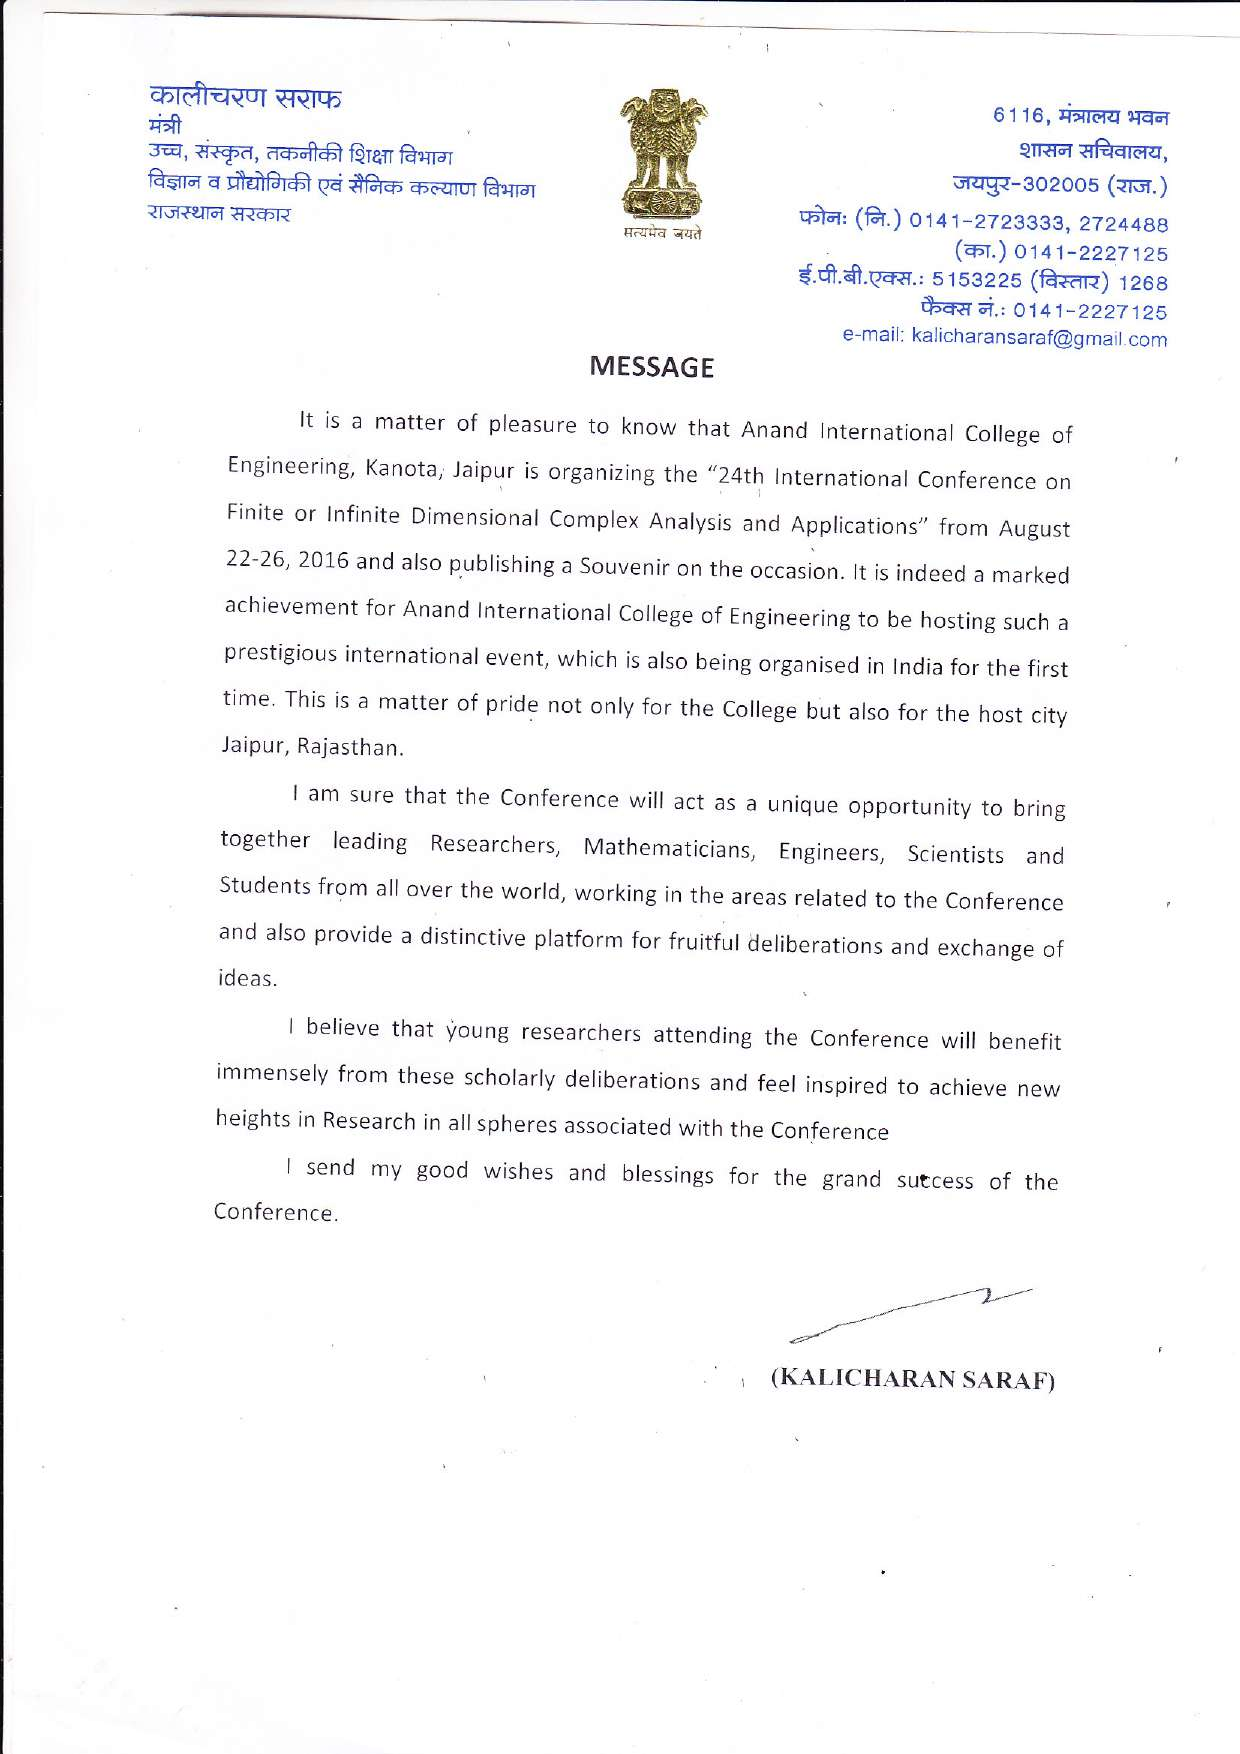
\includepdf[pages=1,pagecommand={\thispagestyle{fancy}},fitpaper]{Message}
%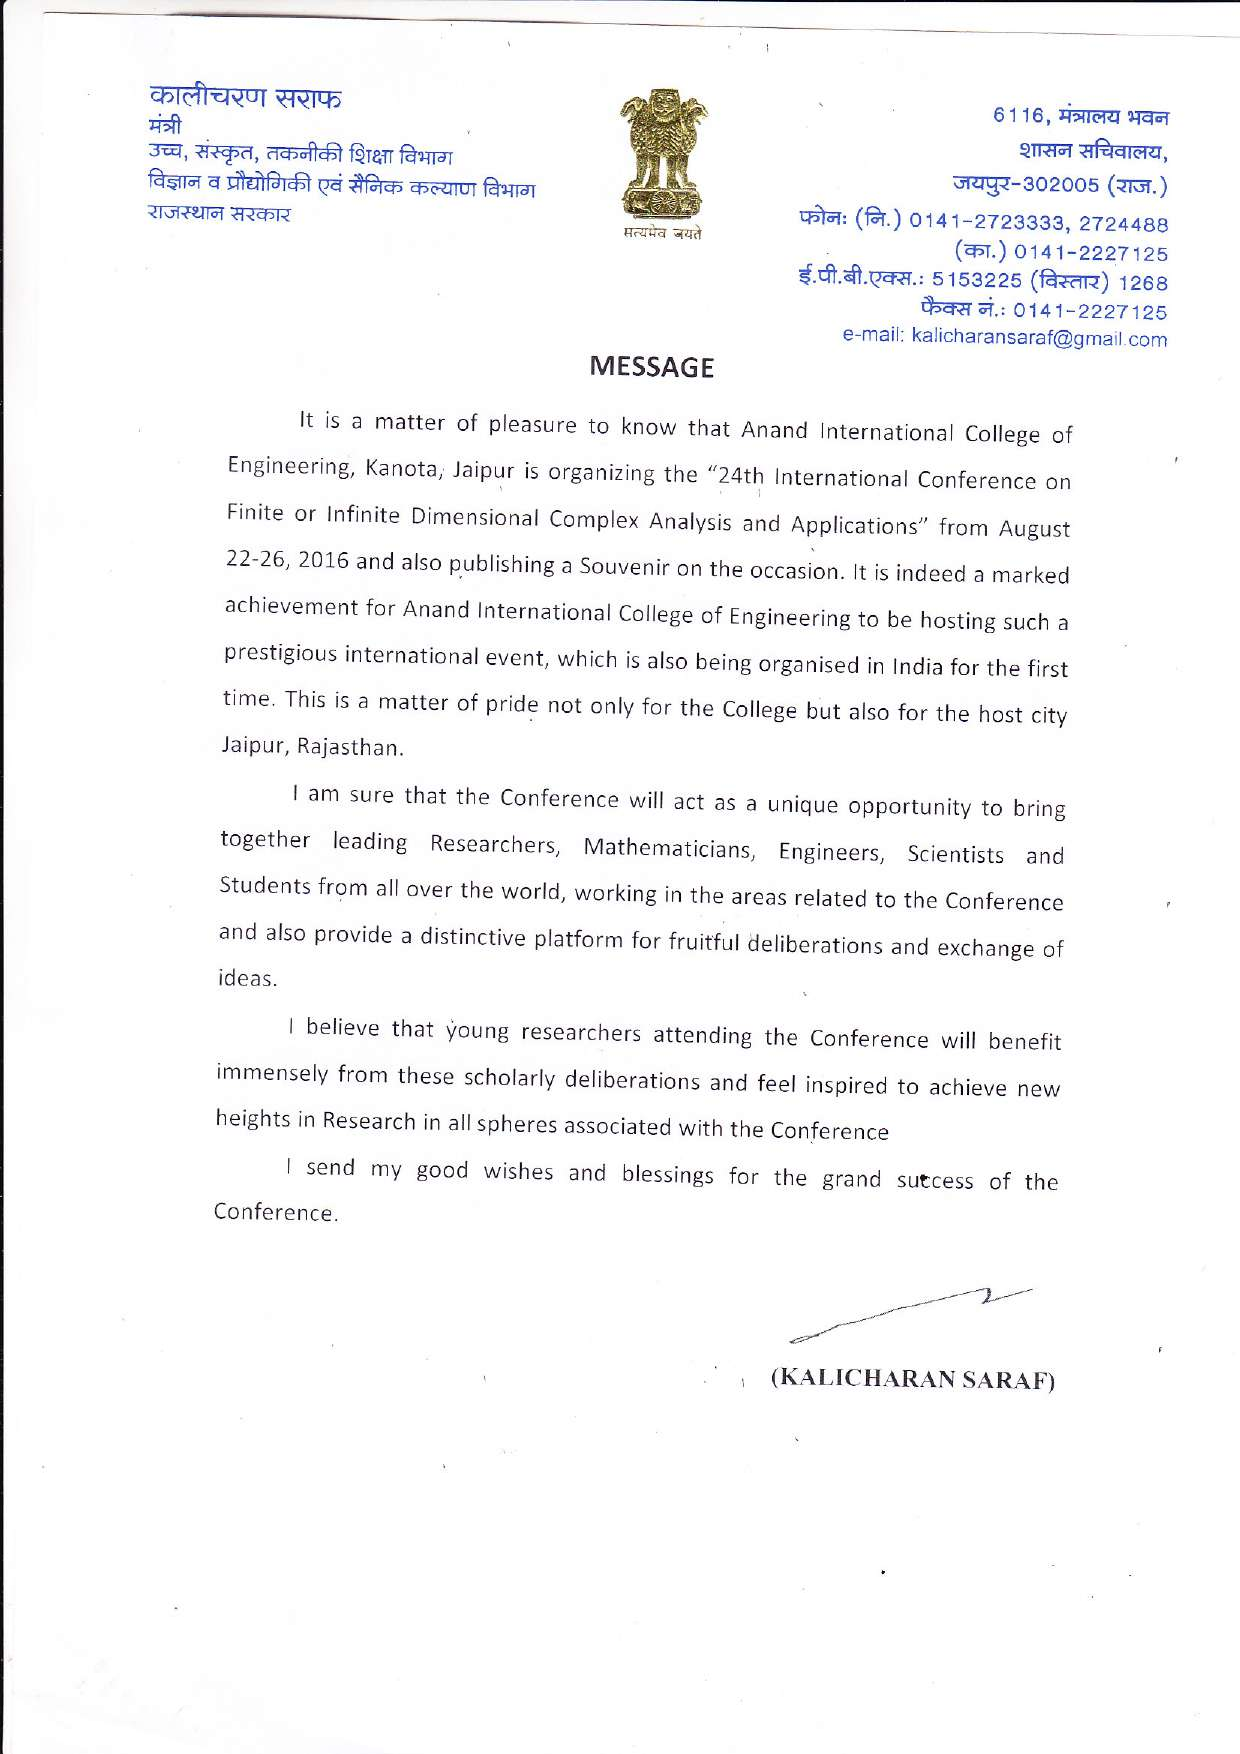
\includepdf[pages=1,frame,scale=0.9,fitpaper=true]{Message}
%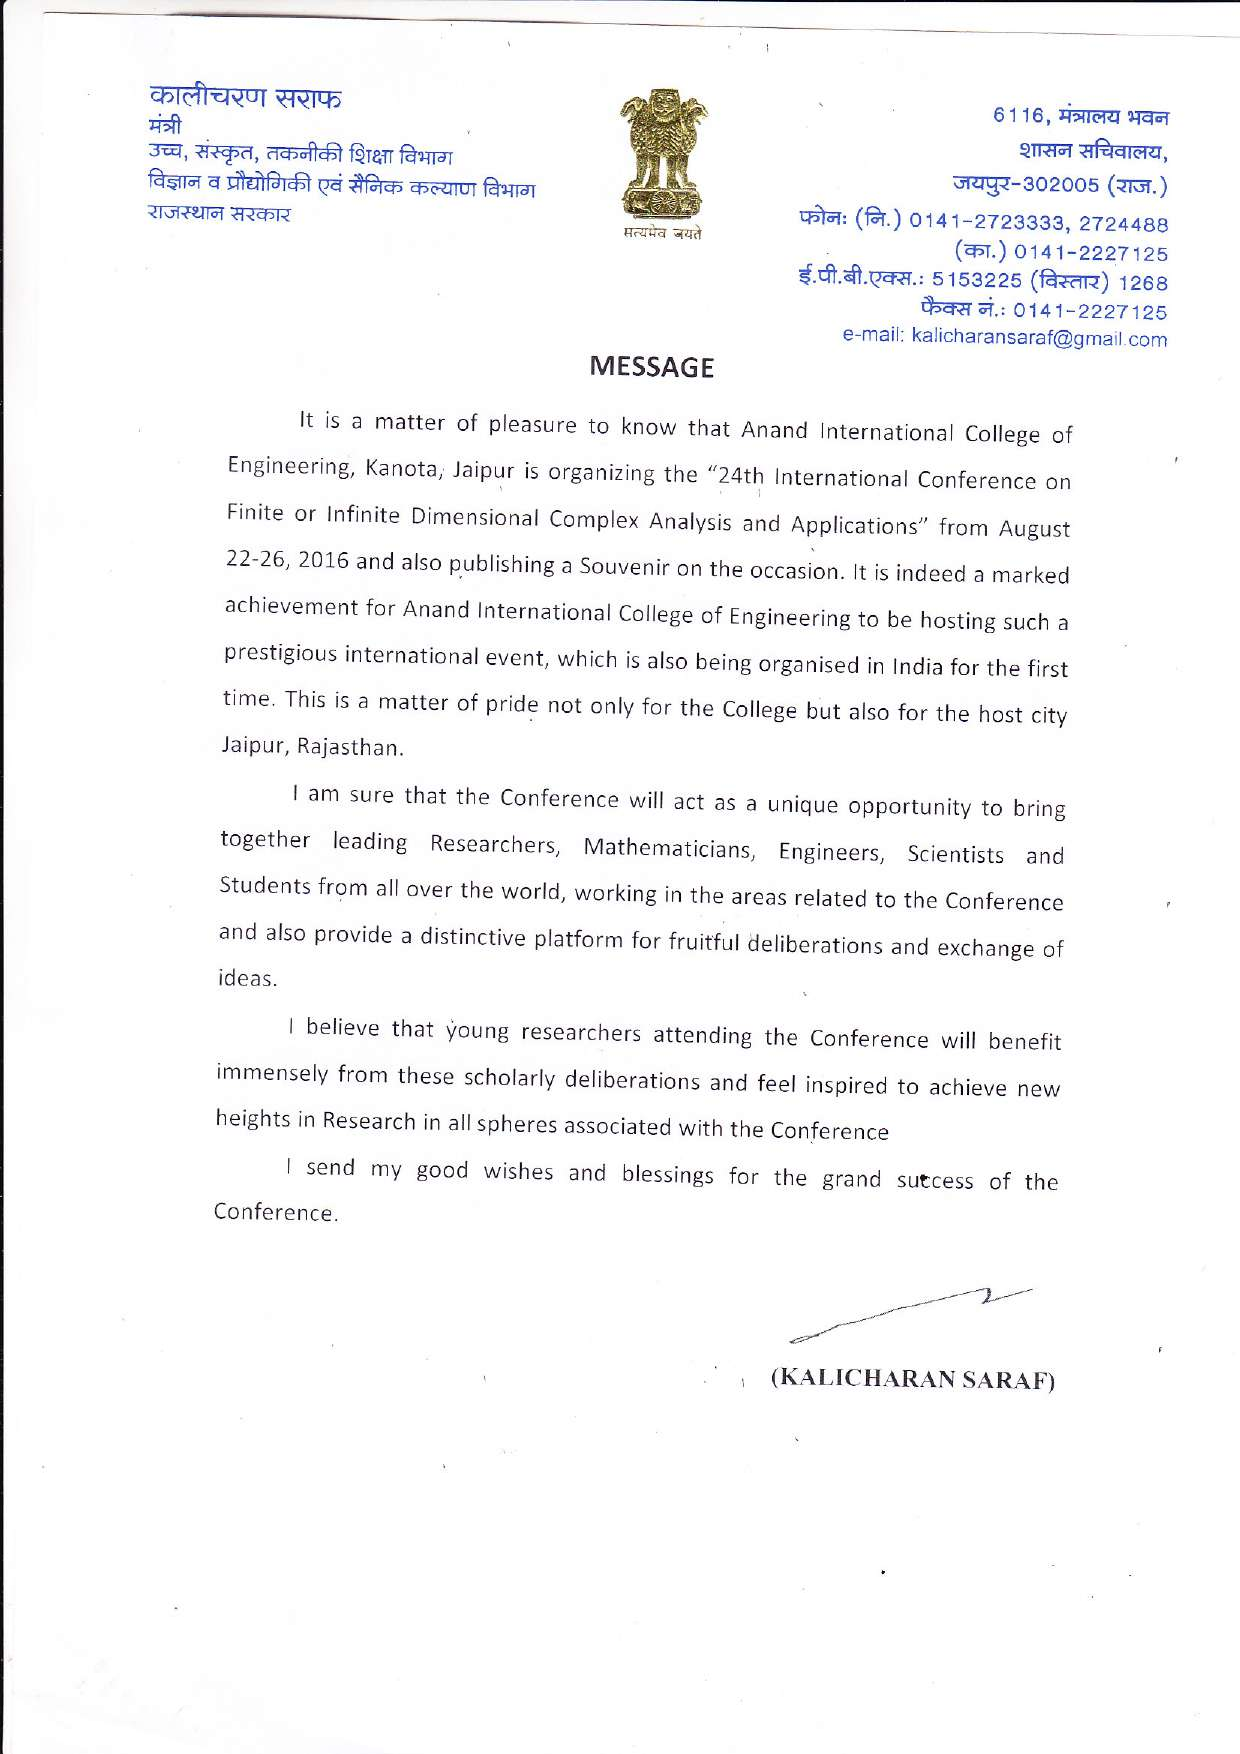
\includepdf[pages=1,pagecommand=\thispagestyle{myheadings}]{Message}
%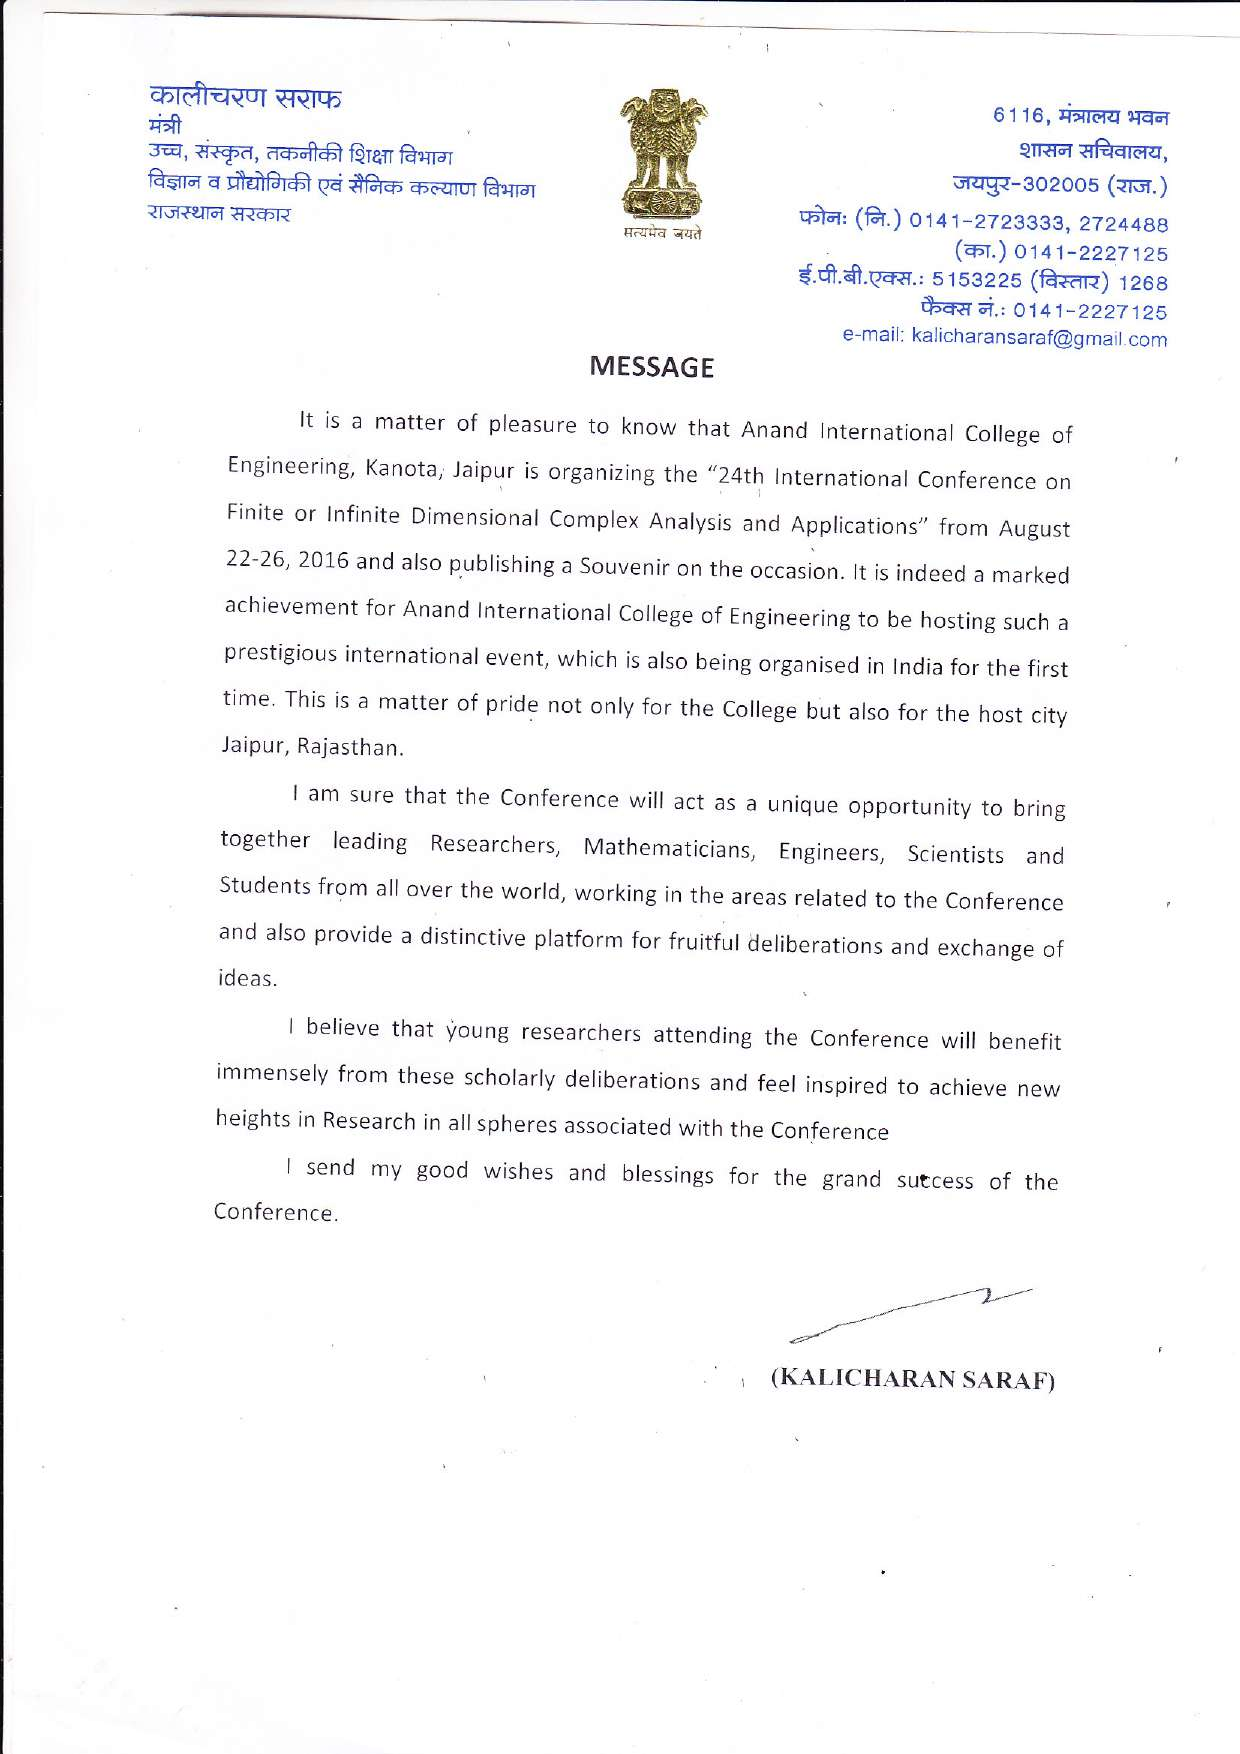
\includepdf[pages=1,frame,scale=0.8]{Message}
\newpage
\begin{flushright}
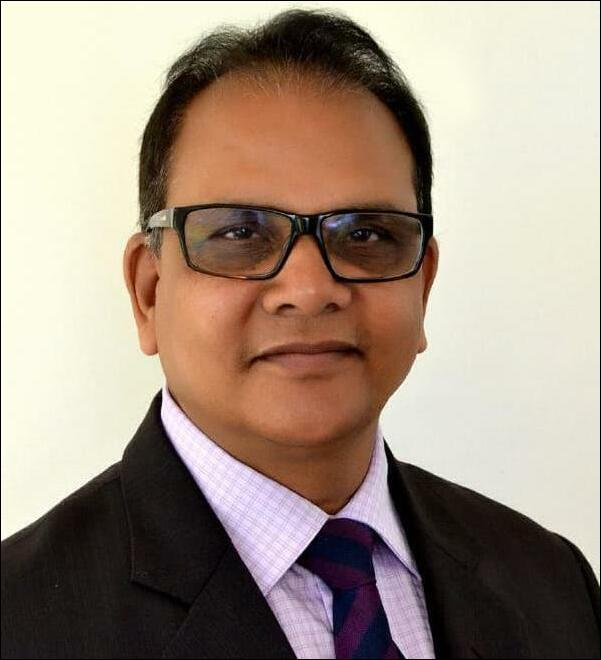
\includegraphics[height=8\baselineskip]{RG1}
\end{flushright}
\vskip 1mm
\hfill \textbf{Prof. R.A Gupta}
\vskip 1mm
\hfill Honorable  Vice Chancellor
\vskip 1mm
\hfill Rajasthan Technical University,Kota
\vskip 10mm
\centerline {\huge{\emph{Message}}}
\vskip 5mm
It is undoubtedly a moment of honor and pleasure to get acquainted with the 3rd International Conference on Recent Development in Engineering \& Technology, ICRDET (Hybrid)-2022 organizing by Anand International College of Engineering, Kanota, Jaipur on 25th and 26th February, 2022 and also publishing a Souvenir on the occasion. The conference is one of its prestigious kinds in the academic field. The conference gives an array of innumerable opportunities to the research scholars, academicians, teachers, scientists, and students to widen their horizon of knowledge to get indulged in the new advancements of the engineering field and bloom like a glorified tech savvy. The college has not only established the milestone among the other colleges across the globe but also provides the pink city and capital of Rajasthan, Jaipur, a moment of pride to organize such an acclaimed international conference.

There have been frequent changes in technology in recent years such as Artificial Intelligent, Quantum Computing, Blockchain Technology and many more. I am confident that this conference would provide a platform to the researchers, academicians and technocrats to move further in this direction.

I would like to congratulate the Management of Anand-ICE, Jaipur for their initiative to organize such kind of scientific activities.  I also appreciate the efforts of Prof. Deepak Bhatia, RTU, Kota and Prof. Praveen Anand-ICE for making this event happen.
My assurance says that the conference would be a tremendous and prodigious learning platform to the fervent participants and encourages more to approach such erudite events in the near future.

My heartwarming and uplifting wishes and blessings are there with the college in the form of massive success of the conference.

\vskip 5mm
%\hskip 10mm \hrule \hskip 10mm
%\rule{\textwidth}{1.5pt}
\newpage
\begin{flushright}
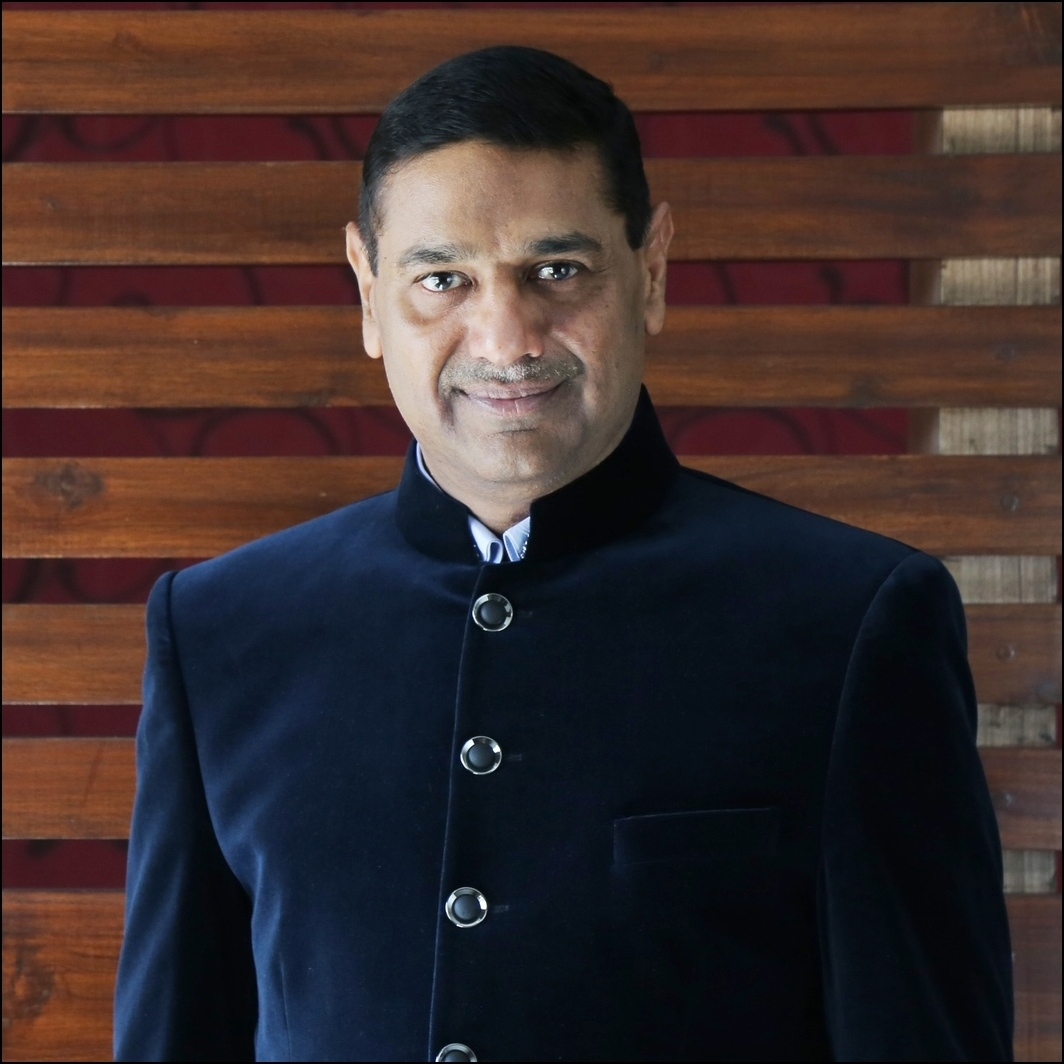
\includegraphics[height=8\baselineskip]{MM}
\end{flushright}
\vskip 1mm
\hfill \textbf{Mr. Manoj Mittal}
\vskip 1mm
\hfill Chairman
\vskip 1mm
\hfill Anand International College of Engineering
\vskip 10mm
\centerline {\huge{\emph{Message}}}
\vskip 5mm
It gives me immense pleasure to welcome you to the ICRDET-2022, being organized at Anand International College of Engineering. It's a privilege to host this International Conference on recent developments in Engineering and Technology.

I am honoured to be a part of Anand International College of Engineering and other divisions of the Anand Group.

Our college is known for its teaching methodology, career-oriented training program, and world class infrastructure. It makes space for creativity and backs innovative and unconventional ideas. Academic excellence in all sectors globally and competitive edge are key elements of Anand College's mission, so that our students can successfully integrate themselves into the global community.

In this light, I am sure that the upcoming convocation of educators and researchers will offer incredible benefits to our students. It will also provide a platform for them to learn internationally.

As Chairman of Anand International College of Engineering, I assure you that I will bring our education sector higher to a level, where the vision of each resident of nation is more clear and they make our nation proud in every industry - technology, management, information technology, etc., not just nationally, but worldwide.

To lighten up the Conference ambiance, I am grateful to have Prof. Praveen Agarwal, Conference General Chair and Prof. Bhavana Mathur, Organizing Chair for taking Anand college on another level in Education sector through their laudable efforts, and would like to extend a special welcome to the International Advisory Board, International Committee Members, National Organizing Committee, Conference Speakers and all the delegates in this Conference.

\vskip 5mm
%\hskip 10mm \hrule \hskip 10mm
%\rule{\textwidth}{1.5pt}
\newpage
\vskip 1mm
\begin{flushright}
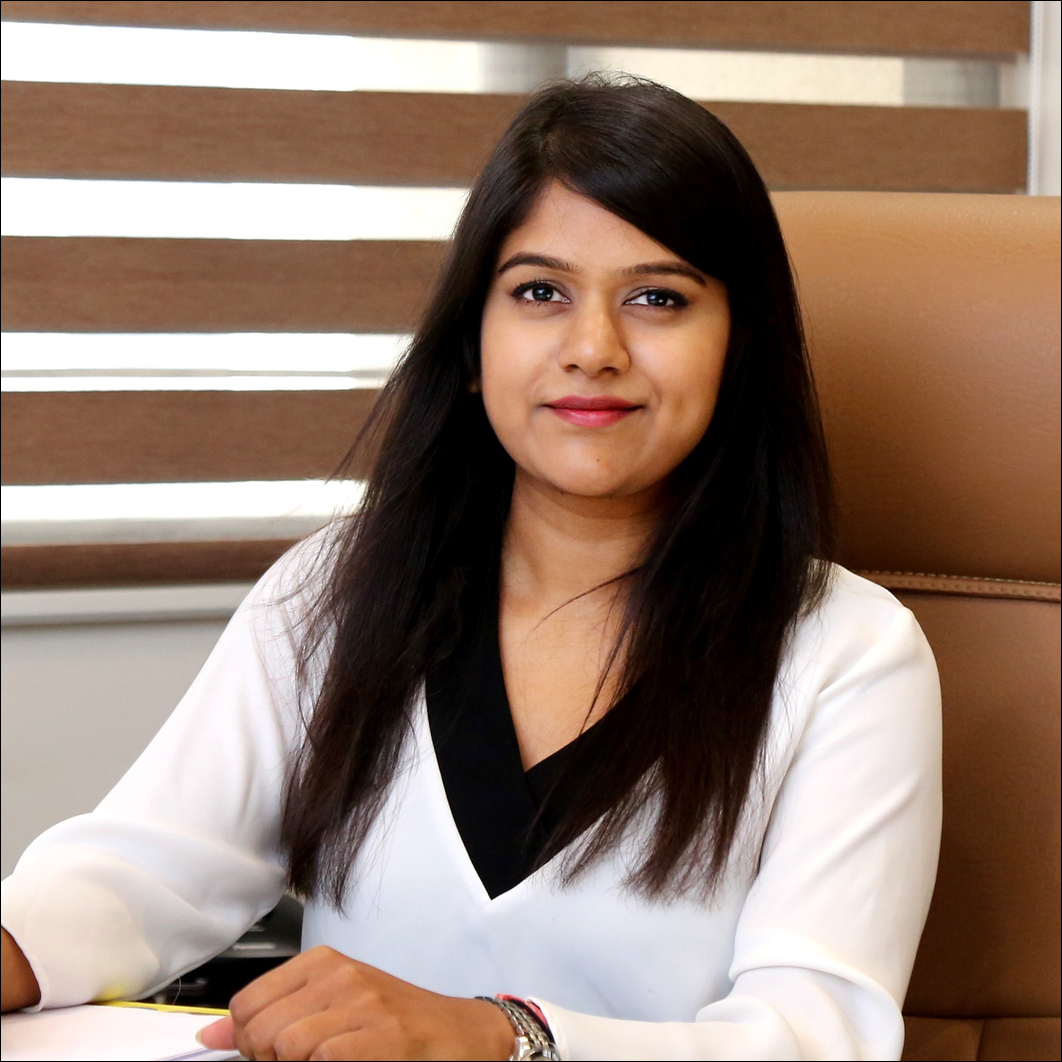
\includegraphics[height=8\baselineskip]{VC}
\end{flushright}
\vskip 1mm
\hfill \textbf{Ms. Monika Mittal}
\vskip 1mm
\hfill Vice Chairperson
\vskip 1mm
\hfill Anand International College of Engineering
\vskip 10mm
\centerline {\huge{\emph{Message}}}
\vskip 5mm
It is a great privilege for Anand International College of Engineering to host the
3rd Hybrid ICRDET - 2022. I would like to extend a warm welcome to all the
International \& National delegates in our Campus. This Conference is an
International platform for the experts in the fields of Mechanical, Civil, Electrical,
Electronics, Computer Engineering \& Basic Sciences, and provide a unique
opportunity for Researchers to share their latest advancements and develop new
collaborations.

Anand International College of Engineering is a unique community of students
and staff dedicated to exchange of ideas and imparting good quality education to
develop in our students a zeal to outshine so that they may steer their
professional careers towards the zenith of Excellence.

This Global exposure will definitely impact the thinking and intellectual
development of our budding engineers. Also, I am sure that we will be able to
satisfy the urge of newer learning and erudite communication among all the
participants in this two-day Conference.

I appreciate the efforts of Prof. Praveen Agarwal and Prof. Bhavana Mathur for
making this event happen in our College, and am also thankful to the dedicated
local team of Programme Committee Members who are constantly striving to
make this event a grand success.

I once again welcome all the participants and hope that they will enjoy their stay
at Jaipur.

Good Luck and my heartiest wishes for the success of this Conference!!
\vskip 5mm
\newpage
\begin{flushright}
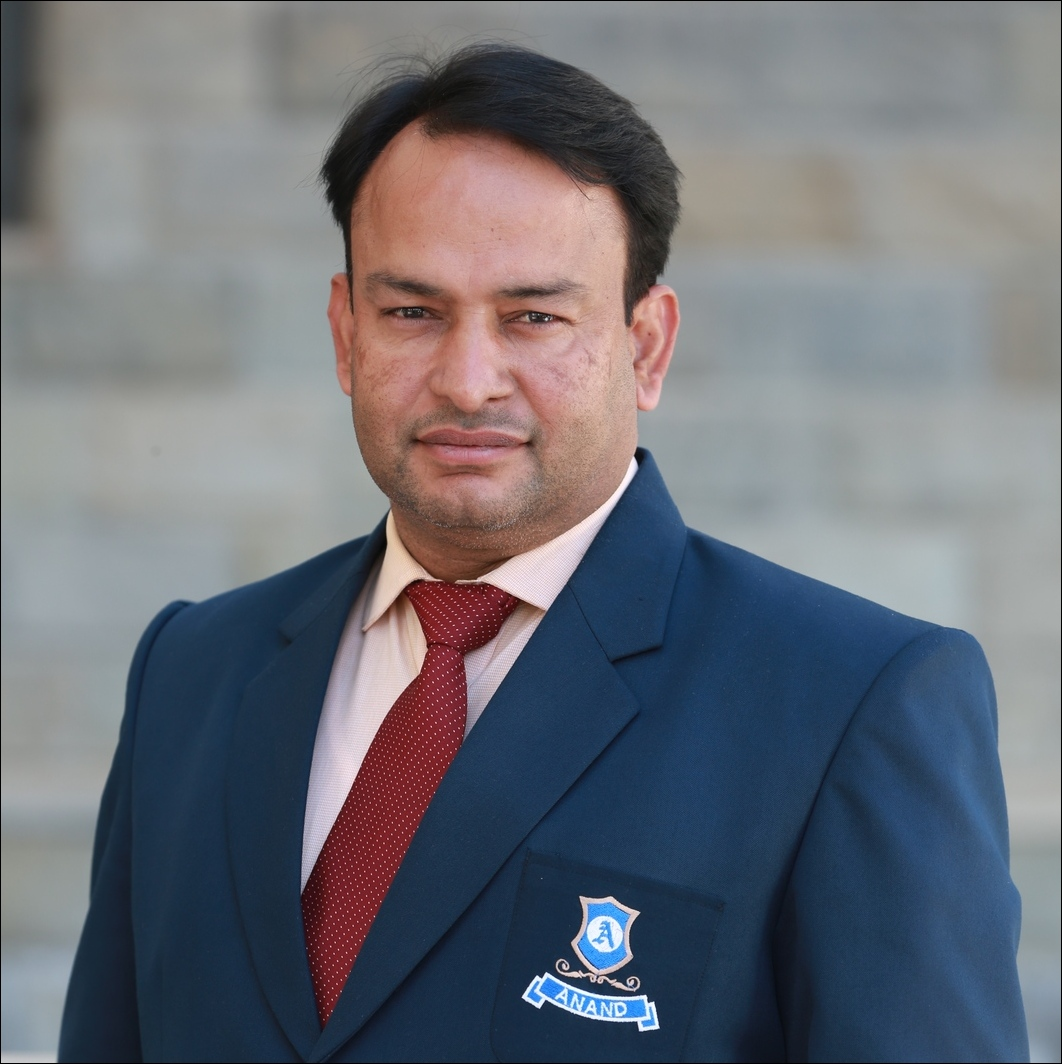
\includegraphics[height=8\baselineskip]{PP}
\end{flushright}
\vskip 1mm
\hfill \textbf{ Prof. Vijay Sharma}
\vskip 1mm
\hfill Principal
\vskip 1mm
\hfill Anand International College of Engineering
\vskip 10mm
\centerline {\huge{\emph{Message}}}
\vskip 10mm
It is quite gratifying to note that Anand International College of Engineering is organizing its Third International Conference on Recent Developments in Engineering and Technology (ICRDET-2022), in association with Rajasthan Technical University, Kota on 25 - 26 February 2022.

Organizing such an event at this point of time reinforces our objective of developing an environment for the exchange of ideas towards technological developments. I wish the conference would be able to deliberate on current issues of national and international relevance, particularly in the field of manufacturing, structural design, data mining, networks, electric systems, big data analytics etc.

There have been unprecedented numbers of quality papers that are to be presented in the conference. I am sure that this occasion will provide an affable environment for the researchers and academicians to freely exchange the views and ideas with others. I convey my warm greetings and felicitations to the organizing committee and the participants and extend my best wishes for the success of the conference.
\vskip 5mm
%\rule{\textwidth}{1.5pt}
\newpage
\vskip 1mm
\begin{flushright}
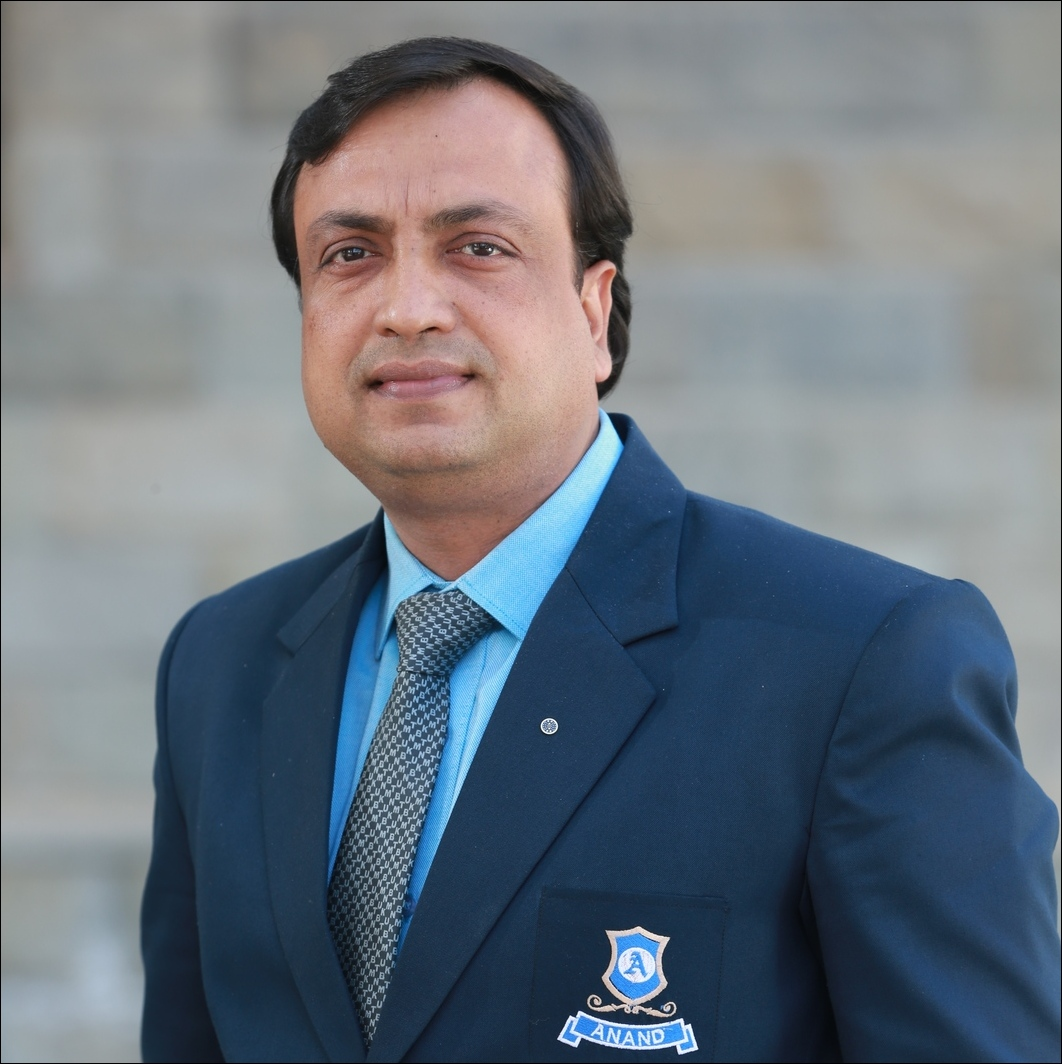
\includegraphics[height=8\baselineskip]{VP}
\end{flushright}
\vskip 1mm
\hfill \textbf{ Prof. Praveen Agarwal}
\vskip 1mm
\hfill Vice Principal
\vskip 1mm
\vskip 1mm
\hfill General Chair-ICRDET-2022
\vskip 1mm
\hfill Anand International College of Engineering
\vskip 10mm
\centerline {\huge{\emph{Message}}}
\vskip 10mm
It is a great pleasure for me to extend a welcome to all of you who are participating in ICRDET-2022, the 3rd International Conference on Recent Development in Engineering \& Technology, which is being held in Anand International College of Engineering, Jaipur, India. The conference is jointly organized by Anand-ICE, Jaipur, India, and RTU, Kota, India.

Due to the Covid-19 Pandemic, many participants could not meet face to face that’s why we decided to make it hybrid by use of technology. In this conference, we bring together researchers and practitioners from academia, industry, and government to exchange their research ideas and results and to discuss the state of the art in the areas of the conference together in a wonderful city of the world, Jaipur.

 There have been quite a big number of applications from different parts of the world and as you know when the number increase task of the organizing committee will increase. Thus it was a very difficult task to select and classify the abstracts for all the participants. We tried to do our best to accommodate many speakers in order to have better and more enjoyable research sessions that will provide more interactions, exchanges among the participants. The talks by eminent speakers and participants will cover a wide range of areas related to the theme of the conference.  We believe that this richness will provide the basis for interdisciplinary collaborations. 
 
 We are also very thankful to all the publishers' to open the special issues for the conference. We also would very much thank all presenters and participants for their interests in the ICRDET 2022 and believe and hope that each of them will get the maximum benefit in terms of networking and interaction from this meeting.
\vskip 1mm
\newpage
We would like to thank the honorable Vice-Chancellor, RTU, Kota (Prof. R. A. Gupta)  for their guidance and support in organizing this conference. Finally, we also would to thank the honorable Chairman (Mr. Manoj Mittal) and Vice-chairperson (Miss Monika Mittal), Anand-ICE, Jaipur for their support and guidance in organizing this Conference Successfully.

Further, we thank all the plenary speakers that kindly accepted our invitation and spend their precious time sharing their ideas during the conference. Also, we are thankful to Principal (Prof. V. K. Sharma), General Chair(Prof. Deepak Bhatia),  Organizing Chairs ( Dr. Harish Sharma and Prof. B. Mathur) and all members of the organizing committee.

We apologize for any shortcomings that might not be mentioned unintentionally or may have been forgotten to be mentioned explicitly here. We really hope for their kind understanding, we thank all and each individual that has put their effort to make this occasion possible.
We welcome each and every one of you again to this conference; we wish you an enjoyable and productive conference and hope to meet again in next ICRDET. 
\vskip 5mm
\newpage
\vskip 1mm
\begin{flushright}
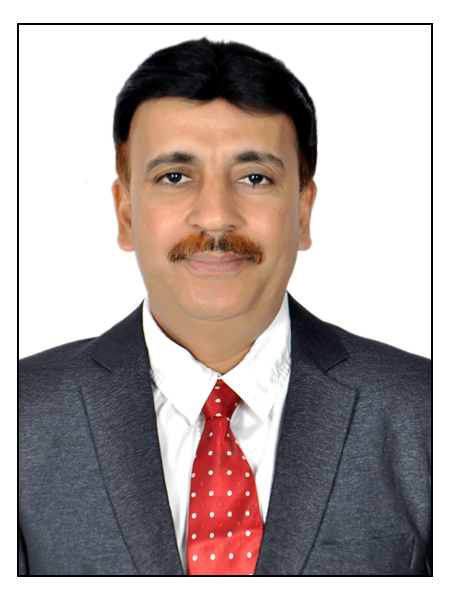
\includegraphics[height=8\baselineskip]{Deepak Bhatia}
\end{flushright}
\vskip 1mm
\hfill \textbf{ Prof Deepak Bhatia}
\vskip 1mm
\hfill General Chair-ICRDET-2022
\vskip 1mm
\hfill  Rajasthan Technical University,Kota
\vskip 10mm
\centerline {\huge{\emph{Message}}}
\vskip 10mm
It’s always been a moment of pride and contentment to be a part of the scholarly learning and this time Anand International College of Engineering, Kanota, Jaipur, has given me this undeniable opportunity to be a part of the 3rd International Conference on Recent Development in Engineering \& Technology, ICRDET (Hybrid)-2022 on 25th and 26th February, 2022 as the General Chair of the conference.

As we are familiar with the objective of 3nd ICRDET-2022 that is to provide a world class platform to present and discuss all the latest research and results of scientists related to Mechanical, Civil, Electrical, Electronics, Computer Engineering and Basic Sciences. Hence, I firmly believe that this conference is going to provide the openings to all the delegates belonging to the different scientific fields to share new ideas and to uncover worldwide cohorts for future alliance.

Anand International College of Engineering, Kanota, Jaipur has always given the untiring efforts in bringing the knowledgeable nectar around the globe by organizing the conferences, seminars, workshop, and other events. This time also the college has nailed their efforts by organizing the 3rd International Conference on Recent Development in Engineering \& Technology, ICRDET (Hybrid)-2022 on 25th and 26th February, 2022. The college has also given me this honor to be a part of the conference as the Organizing Chair.

The conference is going to serve as a tool to all the scholars, academicians, scientists and mathematicians as an update of the technology. The conference will indisputably give the result as the noteworthy contribution to the knowledge in the advancements in the science and technology. The college also offers such an ideal platform for the scholars around the globe every year and I really appreciate such organizations like Anand ICE, Jaipur for putting in such educated endeavors. I am extremely delighted to be a part of such a great conference.
\vskip 1mm
\newpage
\vskip 1mm
I would like to thank the honorable Vice-Chancellor, RTU, Kota (Prof. R. A. Gupta) for their guidance and support in organizing this conference. Further, I would to thank the Prof. Praveen Agarwal his extra ordinary efforts to making this event happen.
I would like to extend my warm thanks to the college for this grand event and an absolute success for it.


My heart is puffed with a sense of gratitude for the college and all the ardent participants who are unquestionably going to make this conference a gigantic success.
\newpage
\vskip 5mm
\begin{flushright}
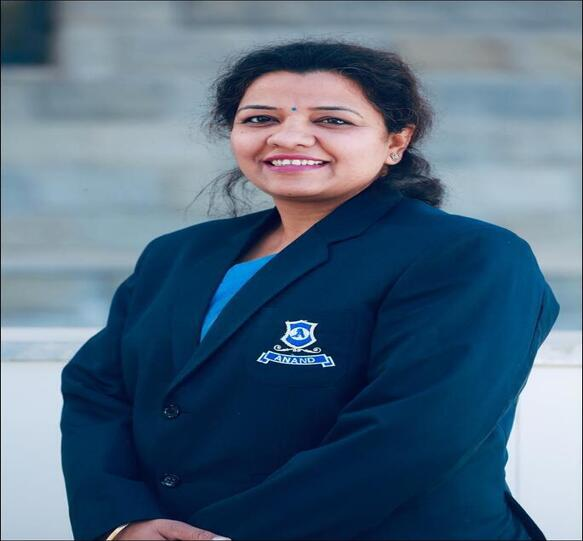
\includegraphics[height=8\baselineskip]{BM2}
\end{flushright}
\vskip 1mm
\hfill \textbf{ Prof. Bhavana Mathur}
\vskip 1mm
\hfill Organizing Chair-ICRDET-2022
\vskip 1mm
\hfill Anand International College of Engineering
\vskip 10mm
\centerline {\huge{\emph{Message}}}
\vskip 10mm
It is extremely a great moment of honor and pleasure to announce for the 3rd International
Conference on Recent Development in Engineering Technology, ICRDET (Hybrid)-2022 jointly
organized by Anand International College of Engineering, Kanota, Jaipur and Rajasthan
Technical University Kota on 25th and 26th February, 2022 and also publishing an Abstract book.

ICRDET is a vast canvas that basically involves independent innovations in Engineering and
science arena as well as from other technical and scientific streams which intuitively provide
excellent opportunities of collaboration to bring about high potentiality for the future.

I extend my heartfelt wishes for the grand success of ICRDET 2022.
\vskip 1mm
\newpage
\vskip 5mm
\begin{flushright}
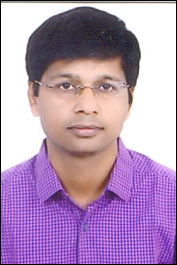
\includegraphics[height=8\baselineskip]{HS}
\end{flushright}
\vskip 1mm
\hfill \textbf{ Prof. Harish Sharma}
\vskip 1mm
\hfill Organizing Chair-ICRDET-2022
\vskip 1mm
\hfill Rajasthan Technical University,Kota
\vskip 10mm
\centerline {\huge{\emph{Message}}}
\vskip 10mm
Anand International College of Engineering, Kanota, Jaipur has always given the untiring efforts in bringing the knowledgeable nectar around the globe by organizing the conferences, seminars, workshop, and other events. This time also the college has nailed their efforts by organizing the 3rd International Conference on Recent Development in Engineering \& Technology, ICRDET (Hybrid)-2022 on 25th and 26th February, 2022. The college has also given me this honor to be a part of the conference as the Organizing Chair.

The conference is going to serve as a tool to all the scholars, academicians, scientists and mathematicians as an update of the technology. The conference will indisputably give the result as the noteworthy contribution to the knowledge in the advancements in the science and technology. The college also offers such an ideal platform for the scholars around the globe every year and I really appreciate such organizations like Anand ICE, Jaipur for putting in such educated endeavors. I am extremely delighted to be a part of such a great conference.

I would like to extend my warm thanks to the college for this grand event and an absolute success for it.

\vskip 1mm












\newpage
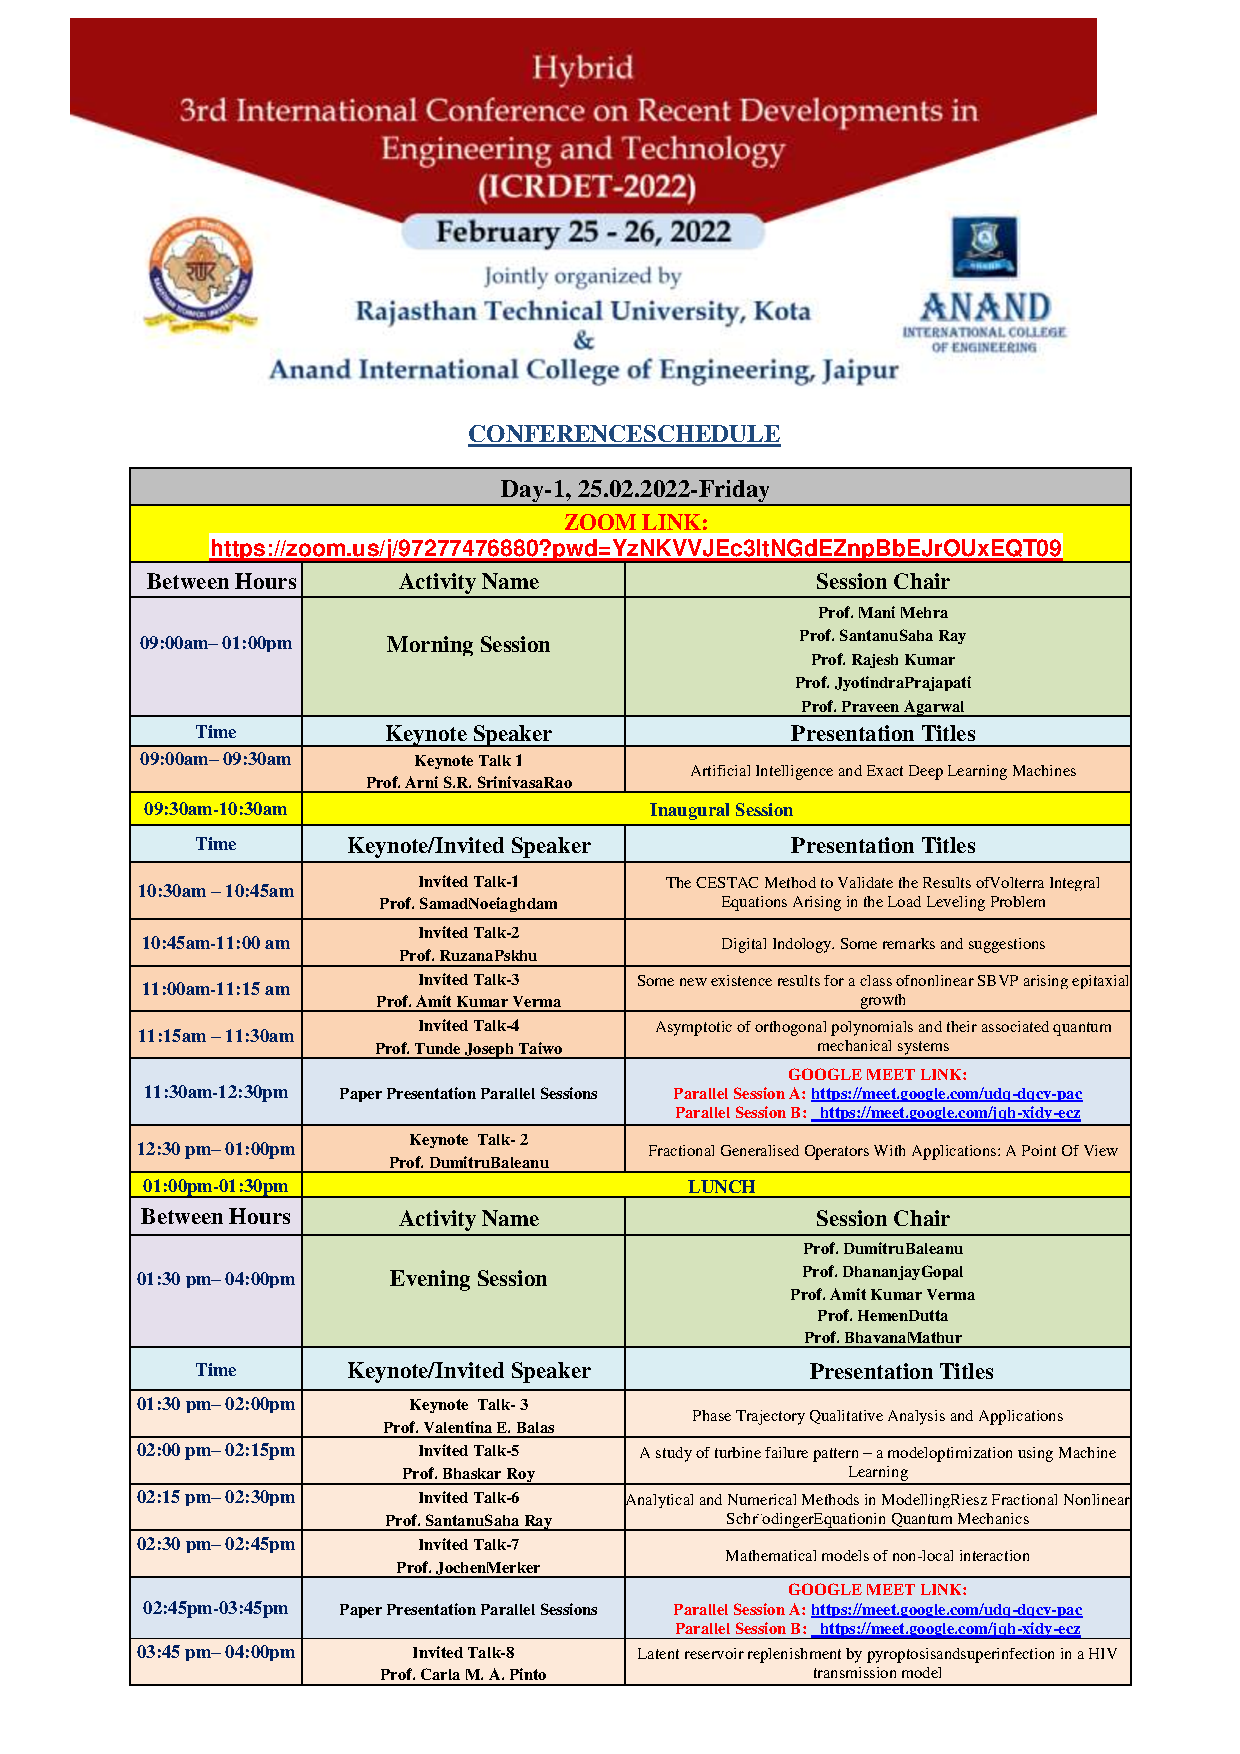
\includepdf[pages=1-5,frame, scale=0.7, pagecommand={}]{Final}
\newpage



\vspace*{85mm}

{\Huge
\begin{center}
Abstracts of Plenary Talks

\end{center}
}



\newpage
%%%%%%%%%%%%%%%%%%%%%%%%%%%%%%%%%%%%%%%%%%%%%%%%%%%%%% OP-001 %%%%%%%%%%%%%%%%%%%%%%%%%%%%%%%%%%%%%%%%%%%%%%%%%%%%%%%%%%%%%%%%%%
\vskip 10mm
\begin{center}\bf\LARGE
Artificial Intelligence and Exact Deep Learning Machines
\end{center}
\vskip 5mm
\begin{center}
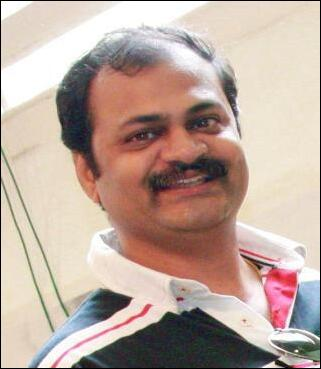
\includegraphics[width=2.5cm, height=2.5cm, keepaspectratio=false]{ASR2.jpg}
\end{center}
\vskip 2mm
\centerline{\textbf{Arni S.R. Srinivasa Rao}}
\vskip 2mm
\begin{flushleft}
Laboratory for Theory and Mathematical Modeling, Medical College of
Georgia, U.S.A.
\end{flushleft}
\vskip 5mm
\begin{flushleft}
\textbf{E-Mail}: arrao@augusta.edu
\end{flushleft}

\vskip 8mm
In this talk, an overview of latest developments and achievements in the
research on AI will be described. Author's work on Exact Deep Learning Machines (EDLMs)
will be explained.
\vskip 2mm
\newpage
%\rule{\textwidth}{0.5pt}
\vskip 2mm
\begin{center}\bf\LARGE
Phase Trajectory Qualitative Analysis and Applications
\end{center}
\vskip 5mm
\begin{center}
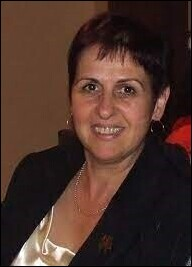
\includegraphics[width=2.5cm, height=2.5cm,keepaspectratio=false]{VEB2.jpg}
\end{center}
\vskip 5mm
\centerline{\textbf{  	Valentina E. Balas }}
\vskip 2mm
\begin{flushleft}
Aurel Vlaicu University of Arad, ROMANIA
\end{flushleft}
\vskip 2mm
\begin{flushleft}
\textbf{E-Mail}: balas@drbalas.ro
\end{flushleft}

\vskip 8mm
The talk presents a soft computing identification method of the operating
regimes for controllers based on the qualitative analyze of the phase trajectory of
the error. The control of highly non-linear and time variable systems demands high
quality self-adaptation. Even we dispose of valid mathematical models for the
controlled plants, the adaptation strategy is inspired by the classic methods from
linear control, like the operational calculus. In most of the real applications we
don’t have valid knowledge about the controlled plant and its mathematical model,
their physical parameters are varying in time and unpredictable external
perturbations may occur. In such cases, the only possible approach that can be
always used is the heuristic one. We propose the phase trajectory of the error as the
basic tool able to support the on-line heuristic adaptive action. The judgments
standing behind the proposed method will be answers to the basic question: “how
would a human operator control and adapt an unknown plant?”.



%\let\thefootnote\relax\footnote{Invited Talk: OP-001\\} %\centerline{\includegraphics*[width=6.2in, height=1in, keepaspectratio=false]{24con.jpg}}}

\newpage
%%%%%%%%%%%%%%%%%%%%%%%%%%%%%%%%%%%%%%%%%%%%%%%%%%% End of Abstract %%%%%%%%%%%%%%%%%%%%%%%%%%%%%%%%%%%%%%%%%%%%%%%%%%%%%%%%%%%%




%%%%%%%%%%%%%%%%%%%%%%%%%%%%%%%%%%%%%%%%%%%%%%%%%%%%%% OP-002 %%%%%%%%%%%%%%%%%%%%%%%%%%%%%%%%%%%%%%%%%%%%%%%%%%%%%%%%%%%%%%%%%%
\vskip 10mm
\begin{center}\bf\LARGE
Fractional Generalised Operators With Applications: A Point Of View
\end{center}
\vskip 5mm
\begin{center}
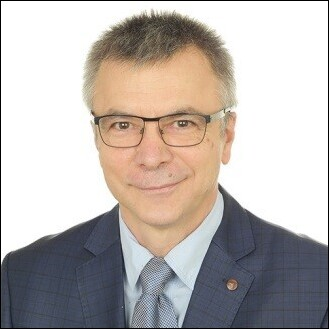
\includegraphics[width=2.5cm, height=2.5cm,keepaspectratio=false]{DB2.jpg}
\end{center}
\vskip 2mm
\centerline{\textbf{  Dumitru Baleanu }}
\vskip 2mm
\begin{flushleft}
Institute of Space Sciences, Magurele-Bucharest, Romania
Cankaya University, Ankara, TURKEY
\end{flushleft}
\vskip 2mm
\begin{flushleft}
\textbf{E-Mail}: dumitru@cankaya.edu.tr
\end{flushleft}

\vskip 8mm
Fractional calculus is an emerging field of mathematics even after 326 years since it was initiated. Among several new direction within this field one is focusing on finding fractional  generalised operators with high potential impact for applications in treating the dynamics of complex systems. In my talk I will discuss some new classes of general operators and I will apply them to solve some real world applications.
\vskip 5mm

\newpage
%%%%%%%%%%%%%%%%%%%%%%%%%%%%%%%%%%%%%%%%%%%%%%%%%%% End of Abstract %%%%%%%%%%%%%%%%%%%%%%%%%%%%%%%%%%%%%%%%%%%%%%%%%%%%%%%%%%%%



%%%%%%%%%%%%%%%%%%%%%%%%%%%%%%%%%%%%%%%%%%%%%%%%%%%%%% OP-003 %%%%%%%%%%%%%%%%%%%%%%%%%%%%%%%%%%%%%%%%%%%%%%%%%%%%%%%%%%%%%%%%%%
\vskip 10mm
\begin{center}\bf\LARGE
Haar Wavelet Fractional Derivative
\end{center}
\vskip 5mm
\begin{center}
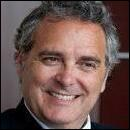
\includegraphics[width=2.5cm, height=2.5cm,keepaspectratio=false]{CC2.jpg}
\end{center}
\vskip 2mm
\centerline{\textbf{ Carlo Cattani }}
\vskip 2mm
\begin{flushleft}
Department Of Economics, Engineering, Society And Business University of Tuscia, ITALY
\end{flushleft}
\vskip 2mm
\begin{flushleft}
\textbf{E-Mail}: cattani@unitus.it
\end{flushleft}
\vskip 8mm
In this lecture the fundamental properties of fractional calculus are discussed with the aim to extend the definition of fractional operators by using wavelets. The Haar wavelet fractional operator is defined, in the more general form, independently on the kernel of the fractional integral.
\vskip 5mm
%\rule{\textwidth}{0.5pt}
\newpage
\vskip10mm
\begin{center}\bf\LARGE
Tetrapods based Smart Materials for Advanced Technologies
\end{center}
\vskip 5mm
\begin{center}
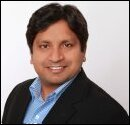
\includegraphics[width=2.5cm, height=2.5cm,keepaspectratio=false]{YKM2.jpg}
\end{center}
\vskip 2mm
\centerline{\textbf{ Yogendra Kumar Mishra }}
\vskip 5mm
\begin{flushleft}

The Mads Clausen Institute, SDU NanoSYD, DENMARK
\end{flushleft}
\vskip 2mm
\begin{flushleft}
\textbf{E-Mail}: mishra@mci.sdu.dk
\end{flushleft}

\vskip 8mm
Considering the size dependent utilization complexities of nanoscopic dimensions towards real applications, the focus of nanomaterials community is merging to three-dimensional (3D) form of materials which are built out interconnected nanostructures. This talk will briefly introduce the importance of complex shaped nanostructures towards smart 3D nanomaterials structuring. A simple flame based single step approach was developed for synthesizing zinc oxide tetrapods which demonstrated many applications in different technologies. These tetrapods have been used as building blocks to construct highly porous interconnected 3D nanonetworks in form of flexible ceramics which offer further new application avenues. Additionally, these 3D networks have been utilized as sacrificial templates to develop hollow tetrapodal 3D networks from almost any desired material, carbons, nitrides, oxides, polymers, hydrogels, etc. The sacrificial template-based strategy offers new and unique opportunities in the direction of 3D nanomaterials engineering and accordingly advanced technological applications. Some examples of 3D nanomaterials engineering will be demonstrated alongwith their applications [1-10]. The scopes of 3D nanostructuring based smart materials in sensing, electronics, optoelectronics, energy, and biomedical engineering will be briefly highlighted in the talk.
\vskip 5mm



\newpage
%%%%%%%%%%%%%%%%%%%%%%%%%%%%%%%%%%%%%%%%%%%%%%%%%%% End of Abstract %%%%%%%%%%%%%%%%%%%%%%%%%%%%%%%%%%%%%%%%%%%%%%%%%%%%%%%%%%%%

%%%%%%%%%%%%%%%%%%%%%%%%%%%%%%%%%%%%%%%%%%%%%%%%%%%%%% OP-004 %%%%%%%%%%%%%%%%%%%%%%%%%%%%%%%%%%%%%%%%%%%%%%%%%%%%%%%%%%%%%%%%%%
\vskip 10mm
\begin{center}\bf\LARGE
Hyers-Ulam and Hyers-Ulam-Rassias Stability of
First-Order Linear and Nonlinear Dynamic Equations
\end{center}
\vskip 5mm
\begin{center}
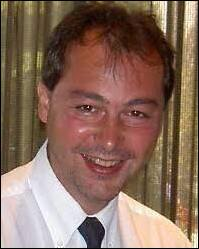
\includegraphics[width=2.5cm, height=2.5cm,keepaspectratio=false]{MB2.jpg}
\end{center}
\vskip 2mm

\centerline{\textbf{  Martin Bohner }}
\vskip 2mm
\begin{flushleft}
Department of Mathematics and Statistics, Missouri University of Science and Technology, Rolla, USA
\end{flushleft}
\vskip 2mm
\begin{flushleft}
\textbf{E-Mail}: bohner@mst.edu
\end{flushleft}

\vskip 10mm
We present several new sufficient conditions for Hyers–Ulam and Hyers–Ulam-Rassias
stability of first-order linear and nonlinear dynamic equations for functions defined on a
time scale with values in a Banach space.
\vskip 5mm
\begin{flushleft}
{\bf }
\end{flushleft}
\newpage
\vskip 10mm
\begin{center}\bf\LARGE
The CESTAC Method to Validate the Results of Volterra Integral Equations Arising in the Load Leveling Problem
\end{center}
\vskip 5mm
\begin{center}
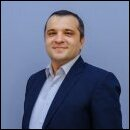
\includegraphics[width=2.5cm, height=2.5cm, keepaspectratio=false]{SN2.jpg}
\end{center}
\vskip 2mm

\centerline{\textbf{  Samad Noeiaghdam }}
\vskip 2mm
\begin{flushleft}
Irkutsk National Research Technical University, Irkutsk, RUSSIA
\end{flushleft}
\vskip 2mm
\begin{flushleft}
\textbf{E-Mail}:  noiagdams@susu.ru
\end{flushleft}

\vskip 8mm
Abstract
The aim of this study is to discuss application of the CESTAC method and the CADNA library to control the accuracy of the Adomian decomposition method and the homotopy perturbation method to solve the linear and nonlinear Volterra integral equations with discontinuous kernel. The importance of solving this problem is be- cause of its applications in the load leveling problems, energy storage with renewable and diesel generation, charge/discharge storages control and others.
In general, the mathematical methods for solving the mentioned problem are based on floating point arithmetic and the accuracy of the method has been discussed using the traditional absolute error which depends on the exact solution and also a positive small value$\epsilon$. But in real life problems we do not have the exact solution. Also, based on this condition we will not be able to find more accurate approximations because we do not have information about optimal $\epsilon$. For small values of $\epsilon$, the numerical algorithm can not be stopped and extra iterations will be produced without improving the accuracy. For large values of $\epsilon$, the numerical algorithm will be stopped in initial steps without producing enough iterations.
Because of the mentioned problems we apply a new termination criterion which depends on two successive approximations. For this aim we apply the CESTAC method and the CADNA library which are based on stochastic arithmetic. In this condition, not only we do not need to have the exact solution but also we would be able to identify the optimal approximation, optimal iteration and optimal error of numerical procedure. Also, the CADNA library is applied as an important software for this validation. The CADNA library should be done on the LINUX operating system and its codes should be written using C, C++ or ADA codes.
\begin{flushleft}
{\bf }
\end{flushleft}
\newpage
%%%%%%%%%%%%%%%%%%%%%%%%%%%%%%%%%%%%%%%%%%%%%%%%%%% End of Abstract %%%%%%%%%%%%%%%%%%%%%%%%%%%%%%%%%%%%%%%%%%%%%%%%%%%%%%%%%%%%

%%%%%%%%%%%%%%%%%%%%%%%%%%%%%%%%%%%%%%%%%%%%%%%%%%%%% OP-005 %%%%%%%%%%%%%%%%%%%%%%%%%%%%%%%%%%%%%%%%%%%%%%%%%%%%%%%%%%%%%%%%%%
\vskip 10mm
\begin{center}\bf\LARGE
Some new existence results for a class of nonlinear SBVP arising epitaxial growth
\end{center}
\vskip 5mm
\begin{center}
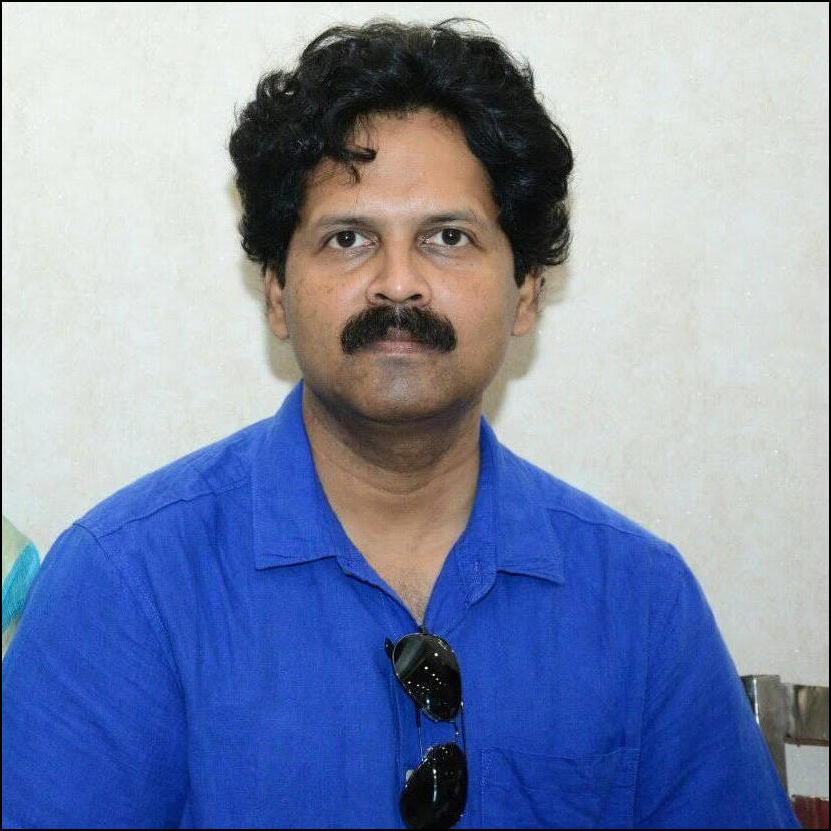
\includegraphics[width=2.5cm, height=2.5cm, keepaspectratio=false]{AKV2.jpg}
\end{center}
\vskip 2mm

\centerline{\textbf{Amit Kumar Verma }}
\vskip 2mm
\begin{flushleft}
Department of Mathematics, Indian Institute of Technology, Patna, INDIA
\end{flushleft}
\vskip 2mm
\begin{flushleft}
{\bf Email:} akverma@iitp.ac.in
\end{flushleft}

\vskip 8mm
Thin films are used in many structures like high-performance RF devices, microwave ICs, solar cells, and many electronic instruments like lasers, diodes, bipolar transistors. The epitaxial growth technique produces these thin films under high vacuum conditions from the crystal in the semiconductor industry. This talk focuses on a fourth-order nonlinear singular boundary value problem that models Epitaxial growth. The existence of solutions will be discussed. We also discuss how depending on a parameter, existence can fail.
\newpage
%%%%%%%%%%%%%%%%%%%%%%%%%%%%%%%%%%%%%%%%%%%%%%%%%%% End of Abstract %%%%%%%%%%%%%%%%%%%%%%%%%%%%%%%%%%%%%%%%%%%%%%%%%%%%%%%%%%%%


%%%%%%%%%%%%%%%%%%%%%%%%%%%%%%%%%%%%%%%%%%%%%%%%%%%%%% OP-006 %%%%%%%%%%%%%%%%%%%%%%%%%%%%%%%%%%%%%%%%%%%%%%%%%%%%%%%%%%%%%%%%%%
\vskip 10mm
\begin{center}\bf\LARGE
Digital Indology. Some remarks and suggestions
\end{center}
\vskip 5mm
\begin{center}
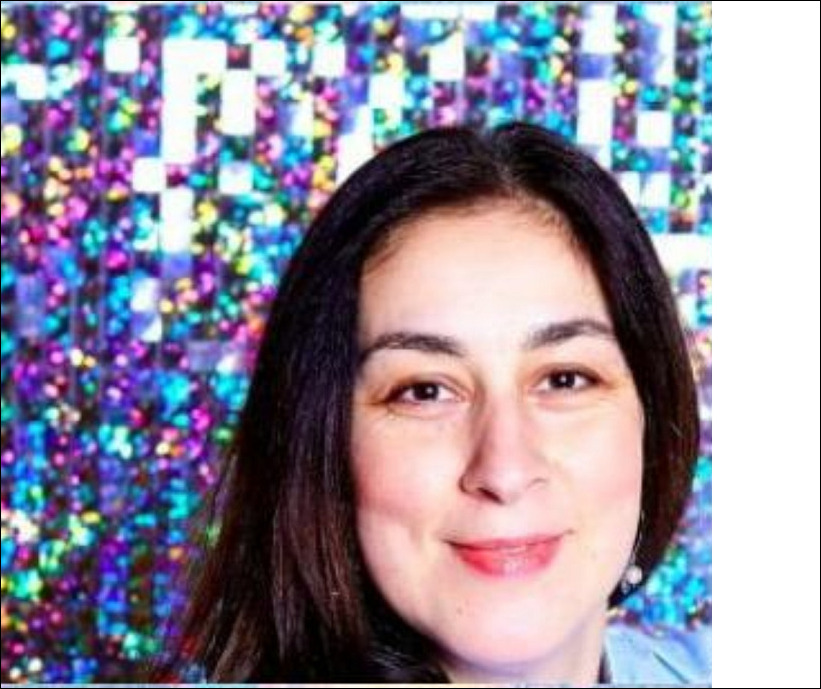
\includegraphics[width=2.5cm, height=2.5cm, keepaspectratio=false]{RP2.jpg}
\end{center}
\vskip 2mm

\centerline{\textbf{  Ruzana Pskhu  }}
\vskip 2mm
\begin{flushleft}
People's Friendship University of Russia (RUDN-University), RUSSIA
\end{flushleft}
\vskip 2mm
\begin{flushleft}
{\bf Email:}  r.pskhu@mail.ru
\end{flushleft}

\vskip 8mm
The paper deals with the research and discussions concerning the active employing the digital instruments and programs in the near-future studies of the Indian intellectual tradition. The term “Digital Indology”, we use here this term by analogue with the term “Digital Humanities”, in the field of the philosophy means investigation of the philosophical textual tradition of Ancient and Medieval India with the using of the digital technology, mathematic statistics, contextual analysis methods and the traditional approaches of the Humanities. The main trends of elaborating the Digital Philosophical Indology (creating the Open Data of Indian Philosophy, elaborating the special programs for ‘reading’ the various Indian shrifts, application of the new methods of analysis of the philosophical texts with the use of digital technologies) are expounded. As the basic methods of analysis of the philosophical texts of India we consider the method of mathematical statistics and the method of contextual analysis. The hidden dangers of using the digital technologies for academical sphere of studies in general and for the intellectual tradition of India in particularly are taken into consideration: sociological intervention, mathematization of the results, minimization of the role of the philosophizing interpretation. The conclusion of such a brief manifest of the Digital Philosophical Indology is declaration of it only as an instrument for the classical Indological studies, which has its own philosophical tasks and aims.
\vskip 5mm
\begin{flushleft}
{\bf }
\end{flushleft}
\newpage
%%%%%%%%%%%%%%%%%%%%%%%%%%%%%%%%%%%%%%%%%%%%%%%%%%% End of Abstract %%%%%%%%%%%%%%%%%%%%%%%%%%%%%%%%%%%%%%%%%%%%%%%%%%%%%%%%%%%%

%%%%%%%%%%%%%%%%%%%%%%%%%%%%%%%%%%%%%%%%%%%%%%%%%%%%%% OP-007 %%%%%%%%%%%%%%%%%%%%%%%%%%%%%%%%%%%%%%%%%%%%%%%%%%%%%%%%%%%%%%%%%%
\vskip 10mm
\begin{center}\bf\LARGE
Machine learning of fractional differential equations

\end{center}
\vskip 5mm
\begin{center}
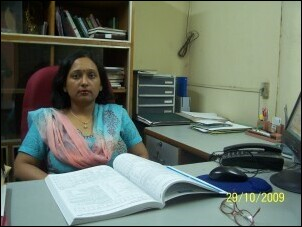
\includegraphics[width=2.5cm, height=2.5cm, keepaspectratio=false]{Mani2.jpg}
\end{center}
\vskip 2mm

\centerline{\textbf{ Mani Mehra }}
\vskip 2mm
\begin{flushleft}
Associate Professor, Department of mathematics, IIT, Delhi, INDIA
\end{flushleft}
\vskip 2mm
\begin{flushleft}
\textbf{E-Mail}: mmehra@maths.iitd.ac.in
\end{flushleft}

\vskip 10mm
We introduce a machine learning framework that uses the differential evolution algorithm in combination with Adam–Bashforth–Moulton method to learn the parameters in a system of variable order fractional differential equations. In this work, we present out developments with regards to taking care of a class of problem: data-driven discovery of system of variable order fractional differential equations.
\vskip 5mm
\newpage
%%%%%%%%%%%%%%%%%%%%%%%%%%%%%%%%%%%%%%%%%%%%%%%%%%% End of Abstract %%%%%%%%%%%%%%%%%%%%%%%%%%%%%%%%%%%%%%%%%%%%%%%%%%%%%%%%%%%%


%%%%%%%%%%%%%%%%%%%%%%%%%%%%%%%%%%%%%%%%%%%%%%%%%%%%%% OP-008 %%%%%%%%%%%%%%%%%%%%%%%%%%%%%%%%%%%%%%%%%%%%%%%%%%%%%%%%%%%%%%%%%%
\vskip 10mm
\begin{center}\bf\LARGE
Asymptotic of orthogonal polynomials and their associated Mechanical systems

\end{center}
\vskip 5mm
\begin{center}
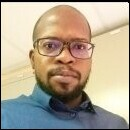
\includegraphics[width=2.5cm, height=2.5cm, keepaspectratio=false]{TJT2.jpg}
\end{center}
\vskip 2mm
\centerline{\textbf{  Tunde Joseph Taiwo }}
\vskip 2mm
\begin{flushleft}
Professor, Department of Physics, United Arab Emirates University, U.A.E
\end{flushleft}
\vskip 2mm
\begin{flushleft}
{\bf Email:} tundetaiwo31@gmail.com
\end{flushleft}

\vskip 5mm
We present a formulation of quantum mechanics based on the theory of orthogonal polynomials. The wave function is expanded over a complete set of square integrable basis where the expansion coefficients are orthogonal polynomials in the energy and physical parameters. Information about the corresponding physical systems (both structural and dynamical) are derived from the properties of these polynomials. We demonstrate that an advantage of this formulation is that the class of exactly solvable quantum mechanical problems becomes larger than in the conventional formulation. We limit our investigation in this work to the Askey classification scheme of hypergeometric orthogonal polynomials and focus on the Wilson polynomial and two of its limiting cases (the Meixner-Pollaczek and continuous dual Hahn polynomials). Nonetheless, the formulation is amenable to other classes of orthogonal polynomials.
\vskip 5mm
%\rule{\textwidth}{0.5pt}
\newpage
\vskip 10mm
\begin{center}\bf\LARGE
An application of neural networks for traffic problems
\end{center}
\vskip 5mm
\begin{center}
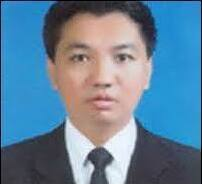
\includegraphics[width=2.5cm, height=2.5cm, keepaspectratio=false]{GR3.jpg}
\end{center}
\vskip 2mm

\centerline{\textbf{ Grienggrai Rajchakit }}
\vskip 2mm
\begin{flushleft}
Department of Mathematics, Faculty of Science, Maejo University, Chiang Mai 50290, THAILAND
\end{flushleft}
\vskip 2mm
\begin{flushleft}
{\bf Email:} kreangkri@mju.ac.th
\end{flushleft}

\vskip 10
Traffic congestion is a thorny issue to many large and medium-sized cities, posing a serious threat to sustainable urban development. Recently, intelligent traffic system (ITS) has emerged as an effective tool to mitigate urban congestion. The key to the ITS lies in the accurate forecast of traffic flow. However, the existing forecast methods of traffic flow cannot adapt to the stochasticity and sheer length of traffic flow time series. To solve the problem, this paper relies on deep learning (DL) to forecast traffic flow through time series analysis. The authors developed a traffic flow forecast model based on the bidirectional Long Short-Term Memory Recurrent Neural Network (BLSTM-RNNs) with delay. The proposed model was compared with two classic forecast models, namely, the autoregressive integrated moving average (ARIMA) model and the Long Short-Term Memory Recurrent Neural Network (LSTM-RNNS) model, through long-term traffic flow forecast experiments, using an actual traffic flow time series from OpenITS. The experimental results show that the proposed BLSTM-RNNs network outperformed the classic models in prediction accuracy. Our research discloses the dynamic evolution law of traffic flow and facilitates the decision-making of traffic management.
\vskip 5mm
\newpage
%%%%%%%%%%%%%%%%%%%%%%%%%%%%%%%%%%%%%%%%%%%%%%%%%%% End of Abstract %%%%%%%%%%%%%%%%%%%%%%%%%%%%%%%%%%%%%%%%%%%%%%%%%%%%%%%%%%%%
%%%%%%%%%%%%%%%%%%%%%%%%%%%%%%%%%%%%%%%%%%%%%%%%%%%%%% OP-009 %%%%%%%%%%%%%%%%%%%%%%%%%%%%%%%%%%%%%%%%%%%%%%%%%%%%%%%%%%%%%%%%%%
\vskip 10mm
\begin{center}\bf\LARGE
Latent reservoir replenishment by pyroptosis and superinfection in a HIV transmission model
\end{center}
\vskip 5mm
\begin{center}

\includegraphics[width=2.5cm, height=2.5cm, keepaspectratio=false]{CMA2.jpg}
\end{center}
\vskip 2mm

\centerline{\textbf{  Carla M.A. Pinto }}
\vskip 2mm
\begin{flushleft}
Instituto Superior de Engenharia do Porto Rua Dr. António Bernardino de Almeida, PORTUGAL
\end{flushleft}
\vskip 2mm
\begin{flushleft}
\textbf{E-Mail}: cap@isep.ipp.pt
\end{flushleft}

\vskip 8mm
We study the role of pyroptosis and super infection on the maintenance of the human immunodeficiency virus (HIV) latent reservoir on infected patients. The proposed model is simulated for biological meaningful parameters and interesting patterns are found. Our results are interpreted for clinical appreciation.
\vskip 5mm
%\rule{\textwidth}{0.5pt}
\newpage
\vskip 10mm
\begin{center}\bf\LARGE
PC-GNN for limb activity recognition
\end{center}
\vskip 5mm
\begin{center}
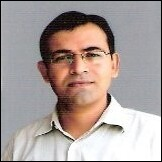
\includegraphics[width=2.5cm, height=2.5cm, keepaspectratio=false]{RK2.jpg}
\end{center}
\vskip 2mm

\centerline{\textbf{  Rajesh Kumar }}
\vskip 2mm
\begin{flushleft}
Department of Electrical Engineering, MNIT, Jaipur, INDIA
\end{flushleft}
\vskip 2mm
\begin{flushleft}
\textbf{E-Mail}: rkumar.ee@mnit.ac.in
\end{flushleft}

\vskip 8mm
In various domains of science and engineering, such as computer vision,
molecular chemistry, molecular biology, pattern recognition, and data mining, graphs
may be used to show many underlying relationships among data. Graph Neural
Networks (GNN) not only gathers individual information, but also uses data from other
samples to create a graph. Graph neural networks are a type of information processing
system that operates by sending messages between graph nodes. GNN variations such
as the graph attention network (GAT), graph convolutional network (GCN), and graph
recurrent network (GRN) have showed revolutionary performance in deep learning and
artificial intelligence applications in recent years. Based on the problems it addresses,
GNN may be classified into three categories: link prediction, node classification, and
graph classification. The proposal is on design of a new Pearson Correlation based
Graph Neural Network (PC-GNN) and to categorize human lower limb activity
recognition.
\vskip 5mm
\newpage
%%%%%%%%%%%%%%%%%%%%%%%%%%%%%%%%%%%%%%%%%%%%%%%%%%% End of Abstract %%%%%%%%%%%%%%%%%%%%%%%%%%%%%%%%%%%%%%%%%%%%%%%%%%%%%%%%%%%%





%%%%%%%%%%%%%%%%%%%%%%%%%%%%%%%%%%%%%%%%%%%%%%%%%%%%%% OP-010 %%%%%%%%%%%%%%%%%%%%%%%%%%%%%%%%%%%%%%%%%%%%%%%%%%%%%%%%%%%%%%%%%%
\vskip 10mm
\begin{center}\bf\LARGE
Physical, hybrid and data-driven modelling techniques of Earth-air heat exchangers for reducing building energy consumption
\end{center}
\vskip 5mm
\begin{center}
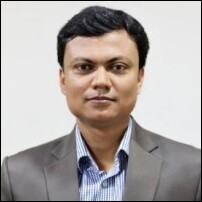
\includegraphics[width=2.5cm, height=2.5cm, keepaspectratio=false]{SFA.jpg}
\end{center}
\vskip 2mm
\centerline{\textbf{  Shams Forruque Ahmed}}
\vskip 2mm
\begin{flushleft}
Professor, Department of Math. \& Computational Sci. Asian University for women, Chittagong, BANGLADESH
\end{flushleft}
\vskip 2mm
\begin{flushleft}
{\bf Email:}  shams.f.ahmed@gmail.com
\end{flushleft}

\vskip 10mm
The development of Earth-Air Heat Exchanger (EAHE) models to reduce building energy use has been notable for the last several decades.However, selecting and executing the most effective EAHE modelling technique in buildings is still a difficulty due to climate, performance, and modelling technique limitations.This paper discusses the available research on several EAHE modelling techniques, including physical, data-driven and hybrid approaches for building applications.Unmeasured disturbances, assumptions, or uncertainties induced in experimental and numerical research of all EAHE modelling methodologies are also discussed.It is demonstrated that hybrid modelling outperforms data-driven and physical models for accurate prediction.However, if EAHE operational circumstances and all essential parameters are included during model building, hybrid models suffer from high complexity.In terms of generality, physical models outperform hybrid and some data-driven models.In addition, a small number of training data is required for physical models, while medium and high numbers are required for hybrid and data-driven models.
\vskip 5mm
%\rule{\textwidth}{0.5pt}
\newpage
\vskip 10mm
\begin{center}\bf\LARGE
Mathematical models of non-local interaction
\end{center}
\vskip 5mm
\begin{center}
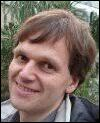
\includegraphics[width=2.5cm, height=2.5cm, keepaspectratio=false]{JM.jpg}
\end{center}
\vskip 2mm

\centerline{\textbf{  Jochen Merker}}
\vskip 2mm
\begin{flushleft}
HTWK Leipzig University of Applied Sciences, GERMANY
\end{flushleft}
\vskip 2mm
\begin{flushleft}
{\bf Email:} jochen.merker@htwk-leipzig.de
\end{flushleft}

\vskip 10mm
Fractional calculus is important because it allows to describe non-local interac-
tions. In this talk, we mathematically discuss two particular possibilities to take
non-local interactions into account. In the first part, we analytically discuss for a
bounded $C^{2}$ domain $\Omega \subset R^{N}$ the semilinear elliptic PDE\\\\
$-\triangle u + c(·, u) = 0$ in $\Omega $ with nonlinearity $c(x, u) := \int_{\partial \Omega}b(x, y, u) dS(y)$\\\\
subject to nonlocal integral Neumann boundary conditions [1]\\
\\
$\frac{\partial d}{\partial \vec{n}} = Iu$ on $\partial \Omega$ with $\int_{\partial \Omega}b(x, y, u(x)) dx$\\\\
modelling non-local interactions between interior points and boundary points. In the
case where the state-dependent kernel $b : \Omega  \times \partial \Omega\times  R \longrightarrow R $ is singular, i.e. where
$b(x, y, u)$ blows up for $\Omega \ni  x \rightarrow y \in \partial \Omega$ so fast that $b(x, y, u) \notin L^{1}(\Omega  \times \partial \Omega)$ for fixed $u \in R$, we prove uniqueness of solutions by invoking duality to linear elliptic PDEs
with fractional divergence as lower order term [2]. In the second part, we consider in
contrast to local finite element methods for the numerical solution of elliptic PDEs
the spectral Bernstein dual Petrov-Galerkin method on a cube $\Omega$ [3]. To use Bernstein
polynomials as non-localized basis functions has some advantages, and we particularly
aim to discuss positivity of solutions for non-negative non-zero data [4].
\vskip 5mm
\newpage
%%%%%%%%%%%%%%%%%%%%%%%%%%%%%%%%%%%%%%%%%%%%%%%%%%% End of Abstract %%%%%%%%%%%%%%%%%%%%%%%%%%%%%%%%%%%%%%%%%%%%%%%%%%%%%%%%%%%%%%%


%%%%%%%%%%%%%%%%%%%%%%%%%%%%%%%%%%%%%%%%%%%%%%%%%%%%% OP-011 %%%%%%%%%%%%%%%%%%%%%%%%%%%%%%%%%%%%%%%%%%%%%%%%%%%%%%%%%%%%%%%%%%
\vskip 10mm
\begin{center}\bf\LARGE
A study of turbine failure pattern – a model optimization using Machine Learning
\end{center}
\vskip 5mm
\begin{center}
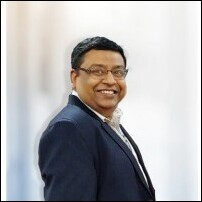
\includegraphics[width=2.5cm, height=2.5cm, keepaspectratio=false]{BR.jpg}
\end{center}

\centerline{\textbf{ Bhaskar Roy }}
\vskip 2mm
\begin{flushleft}
Department of Statistics, Banaras Hindu University, INDIA
\end{flushleft}
\vskip 2mm
\begin{flushleft}
{\bf Email:} bhaskar1974.br@gmail.com
\end{flushleft}

\vskip 5mm
With the growing demand of electricity worldwide, most of the power generation companies focus on long-term and cost-effective asset operation and maintenance strategies to reduce their unplanned downtime which is their main cost driver. Power generating companies are trying to make their commercial process smart and agile enough to do proactive equipment assessment and failure identification in advance rather than taking corrective actions after an event. A turbine failure occurs when a turbine unexpectedly stops producing power due to malfunctioning or break-down of the key components. This creates a complete shutdown of the power generation process and disruption in power generation.
To keep these operational, it is extremely important to have a robust asset reliability and failure prediction models which can pro-actively help these companies to manage their operation and maintenance costs optimally. In this paper, we have studied the failure pattern of turbines after fitting most commonly used single distribution (such as Weibull, gamma and log-normal) and also composite and mixed distributions by the help of machine learning tools to forecast asset failure patterns more accurately. The paper finally compares between single distribution model fitting with composite and mixed distribution model fitting. The numerical illustration is based on historical failure data of 2470 turbines.
More importantly, if more than one suitable model exists, the same can be mathematically combined to get a joint forecast model to forecast failure pattern which is found better than single distribution applied separately. Finally, these predictive methods could be applied to a power generating company for the failure forecast of its assets and to identify upcoming commercial action in advance.
%\vskip 5mm
%\rule{\textwidth}{0.5pt}
\newpage
\begin{center}\bf\LARGE
Analytical and Numerical Methods in Modelling Riesz Fractional Nonlinear Schr\"{o}dinger Equation in Quantum Mechanics
\end{center}
\vskip 5mm
\begin{center}
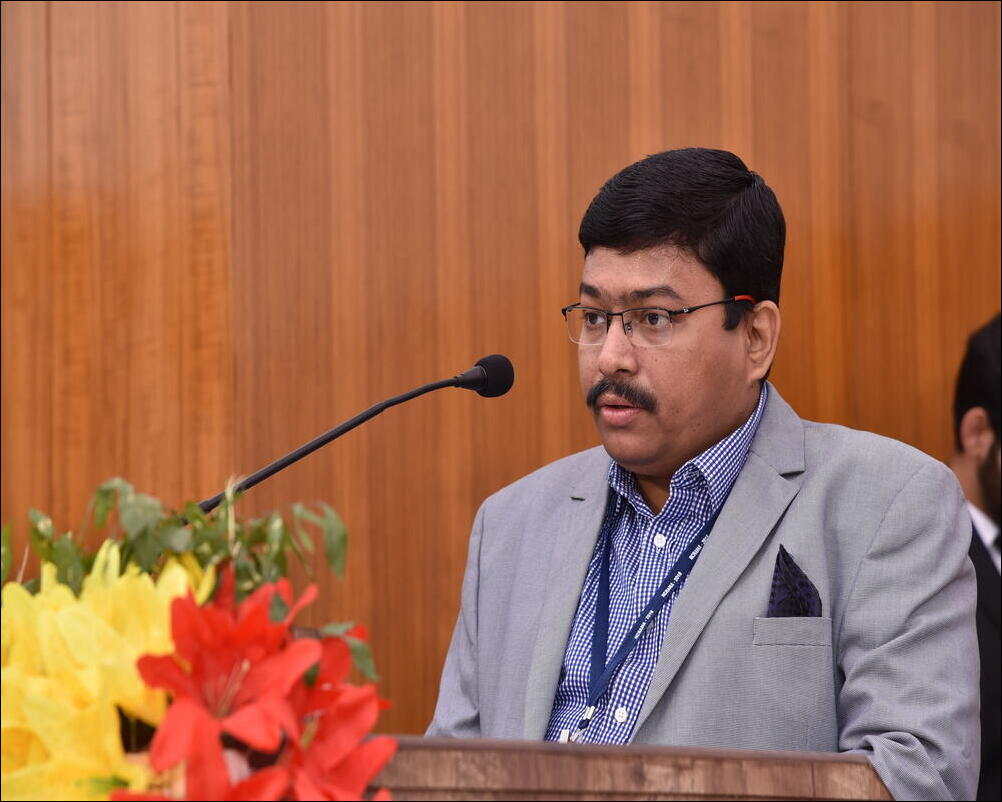
\includegraphics[width=2.5cm, height=2.5cm, keepaspectratio=false]{SSR3.jpg}
\end{center}
\vskip 5mm
\centerline{\textbf{ Santanu Saha Ray }}
\vskip 2mm
\begin{flushleft}
Department of Mathematics, National Institute of Technology, Rourkela, INDIA
\end{flushleft}
\vskip 2mm
\begin{flushleft}
{\bf Email:} santanusaharay@yahoo.com
\end{flushleft}

\vskip 8mm
Analytical and numerical methods for solving the one-dimensional Rieszspace fractional
Schr\"{o}dinger equation are presented in thecase of a particle moving in a potential field. The
fractional derivative is defined by the quantum Riesz fractional derivative. In this respect, a
nonlinear Schrödinger equation with the Riesz fractional derivative has been considered. This
equation has been solved by two reliable methods in order to investigate the accuracy of the
solutions. In the implicit finite difference numerical scheme, the fractional centered difference is
utilized to approximate the Riesz fractional derivative. Also a novel modified optimal homotopy
asymptotic method with Fourier transform (MOHAM-FT) has been proposed to compute the
approximate solution of Riesz fractional nonlinear Schrödinger equation. Further the numerical
solutions obtained by proposed implicit finite difference method, have been compared with that
obtained by MOHAM-FT to exhibit the effectiveness of the suggested methods. Finally, the
obtained solutions have been presented graphically to justify the efficiency of the methods.
\vskip 2mm
\newpage
%%%%%%%%%%%%%%%%%%%%%%%%%%%%%%%%%%%%%%%%%%%%%%%%%%% End of Abstract %%%%%%%%%%%%%%%%%%%%%%%%%%%%%%%%%%%%%%%%%%%%%%%%%%%%%%%%%%%%


%%%%%%%%%%%%%%%%%%%%%%%%%%%%%%%%%%%%%%%%%%%%%%%%%%% OP-012 %%%%%%%%%%%%%%%%%%%%%%%%%%%%%%%%%%%%%%%%%%%%%%%%%%%%%%%%%%%%%%%%%%
\vskip 10mm
\begin{center}\bf\LARGE
Volterra Integral Equation and its solution
\end{center}
\vskip 5mm
\begin{center}
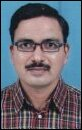
\includegraphics[width=2.5cm, height=2.5cm, keepaspectratio=false]{JP2.jpg}
\end{center}
\vskip 2mm

\centerline{\textbf{  Jyotindra Prajapati }}
\vskip 2mm
\begin{flushleft}
Department of Mathematics, Sardar Patel University, Gujarat, INDIA
\end{flushleft}
\vskip 2mm
\begin{flushleft}
{\bf Email:} jyotindra18@rediffmail.com
\end{flushleft}

\vskip 8mm
Volterra Integral Equation plays an important role in Mathematical Sciences/Mathematical Physics. Laplace transform, Inverse Laplace Transform and their various properties used as a tool to discussed solution of Volterra Integral Equation.
\vskip 5mm
%\rule{\textwidth}{0.5pt}
\newpage
\vskip 10mm
\begin{center}\bf\LARGE
On The Topology of non-triangular metric spaces and related fixed point results
\end{center}
\vskip 5mm
\begin{center}
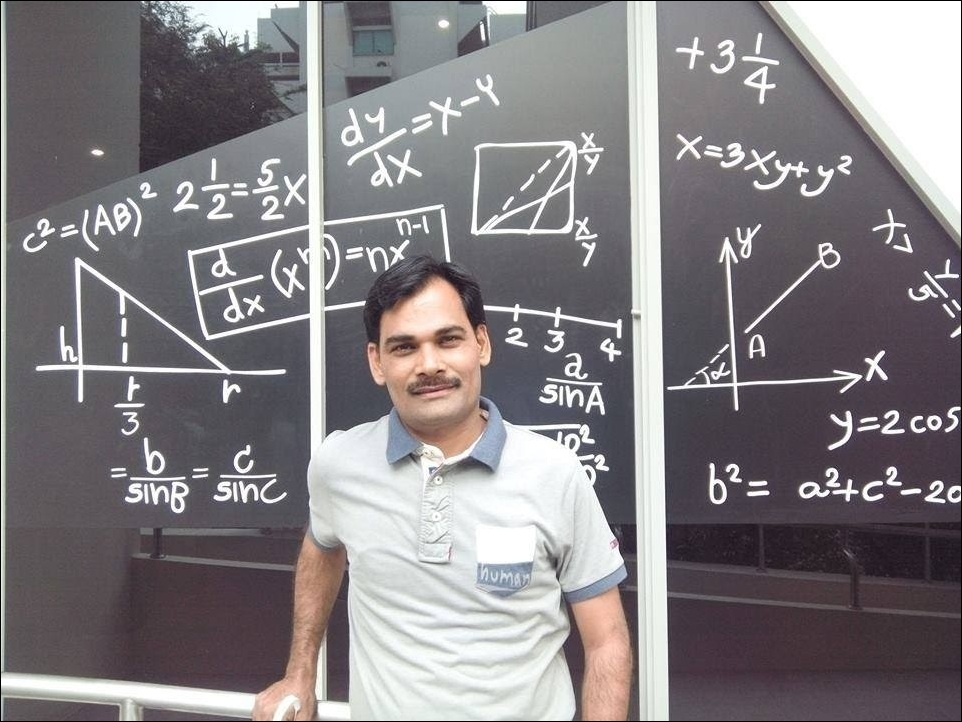
\includegraphics[width=2.5cm, height=2.5cm, keepaspectratio=false]{DG2.jpg}
\end{center}
\vskip 2mm

\centerline{\textbf{  Dhananjay Gopal }}
\vskip 5mm
\begin{flushleft}
Department of Mathematics, Guru Ghasidas Vishwavidyalaya (A Central University), Chhattisgarh, INDIA
\end{flushleft}
\vskip 5mm
\begin{flushleft}
{\bf Email:} gopal.dhananjay@ggu.ac.in
\end{flushleft}

\vskip 10mm
Non-triangular metric spaces have been introduced by Khojasteh and Khandani ([13]) in 2020. The concept of non-triangular metric spaces is fresh and therefore, requires quite some analysis on its topology. In this talk, we shall discuss about the topology of non-triangular metric spaces by giving a natural definition of open sets in this context. The introduction of non-triangular metric spaces has shown that there is no inherent need for the triangle inequality to prove various fixed point results. Keeping this in mind, we give a fixed point result for Suzuki type Z-contractions in the context of non-triangular metric spaces by introducing a new property of maps. We also see the scope of further work on this topic.
\vskip 5mm
\newpage
%%%%%%%%%%%%%%%%%%%%%%%%%%%%%%%%%%%%%%%%%%%%%%%%%%% End of Abstract %%%%%%%%%%%%%%%%%%%%%%%%%%%%%%%%%%%%%%%%%%%%%%%%%%%%


%%%%%%%%%%%%%%%%%%%%%%%%%%%%%%%%%%%%%%%%%%%%%%%%%%%%% OP-013 %%%%%%%%%%%%%%%%%%%%%%%%%%%%%%%%%%%%%%%%%%%%%%%%%%%%%%%%%%%%%%%%%%
\vskip 10mm
\begin{center}\bf\LARGE
Effects of generalized thermal transport on the unsteady convective flows over a vertical cylinder with time-dependent temperature
\end{center}
\vskip 5mm
\begin{center}
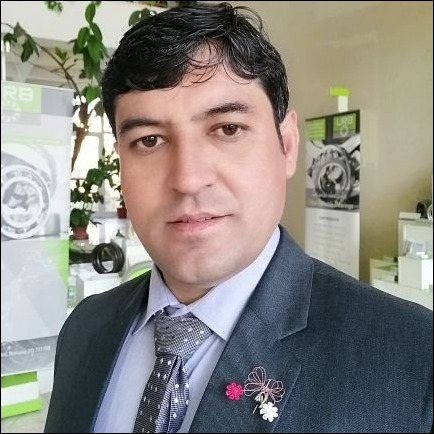
\includegraphics[width=2.5cm, height=2.5cm, keepaspectratio=false]{NA2.jpg}
\end{center}
\vskip 2mm

\centerline{\textbf{ Nehad Ali Shah }}
\vskip 2mm
\begin{flushleft}
Department of Mechanical Engineering, Sejong University, KOREA
\end{flushleft}
\vskip 2mm
\begin{flushleft}
{\bf Email:} nehadali199@yahoo.com
\end{flushleft}

\vskip 10mm
An analysis is made for the generalized transient convective flows over an infinite, vertical, heated circular cylinder. The generalization considers a new form of the constitutive equation of the thermal flux based on the generalized time-fractional derivative with Mittag-Leffler kernel, called the generalized Atangana-Baleanu derivative.Closed forms of the analytical solutions for the temperature and velocity fields, expressed with Bessel and Struve functions, are determined using the Laplace transform and the Weber-Dirichlet transform.The solutions obtained for the generalized case are suitable for particularizations to give solutions corresponding to fractional derivatives with power-law kernel and exponential kernel. The ordinary case corresponding to classical Fourier's law is also obtained.Numerical simulations obtained with the software Mathcad are carried out and graphically illustrated in order to compare models based on generalized Atangana-Baleanu, Atangana-Baleanu, Caputo, and Caputo-Fabrizio time-fractional derivatives.
\vskip 5mm
\newpage
%%%%%%%%%%%%%%%%%%%%%%%%%%%%%%%%%%%%%%%%%%%%%%%%%%% End of Abstract %%%%%%%%%%%%%%%%%%%%%%%%%%%%%%%%%%%%%%%%%%%%%%%%%%%%%%%%%%%%



%%%%%%%%%%%%%%%%%%%%%%%%%%%%%%%%%%%%%%%%%%%%%%%%%%%%%%%%%%%%%% OP-014 %%%%%%%%%%%%%%%%%%%%%%%%%%%%%%%%%%%%%%%%%%%%%%%%%%%%%%%%%%%
\vskip 10mm
\begin{center}\bf\LARGE
Understanding the structure of a machine brain
\end{center}
\vskip 5mm
\begin{center}
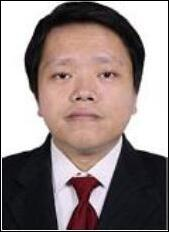
\includegraphics[width=2.5cm, height=2.5cm, keepaspectratio=false]{Wang2.jpg}
\end{center}
\vskip 2mm

\centerline{\textbf{ Wen-Feng Wang }}
\vskip 2mm
\begin{flushleft}
Shanghai Institute of Technology, CHINA
\end{flushleft}
\vskip 2mm
\begin{flushleft}
{\bf Email:} wangwenfeng@iimtcair.edu.in
\end{flushleft}
\vskip 10mm
This article explains the reason why we interpret the structure of a machine brain as a five-layer intelligence. First, we review the physiological structure of the human brain. About 80\% of a human brain are water, and the others are complex biochemical structures. It is almost impossible to simulate the physiological structure of the human brain. Second, we analyze the functional mechanisms of the human brain, including a preliminary understanding of the connections between neurons in the brain. The role of synapses is also discussed. It is possible to simulate the learning mechanisms of a human brain. Finally, we present a framework to carry out such simulation by summarizing the current level of machine intelligence as a “five-layer intelligence”. Explicit functional mechanisms and practical examples of the five intelligence layers, along with trends in machine intelligence and the role of nonlinear science, are also further interpreted.
\vskip 5mm
%\rule{\textwidth}{0.5pt}
\newpage
\vskip 10mm

\begin{center}\bf\LARGE
An introduction to functional equations and their stability analysis
\end{center}
\vskip 5mm
\begin{center}
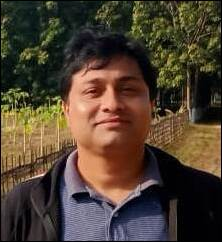
\includegraphics[width=2.5cm, height=2.5cm, keepaspectratio=false]{HD2.jpg}
\end{center}
\vskip 2mm

\centerline{\textbf{ Hemen Dutta }}
\vskip 2mm
\begin{flushleft}
Department of Mathematics and Statistics, Gauhati university, Guwahati, INDIA
\end{flushleft}
\vskip 2mm
\begin{flushleft}
{\bf Email:} duttah@gauhati.ac.in
\end{flushleft}
\vskip 10mm
This talk is about functional equations, or the search for functions that satisfy certain
functional relationships. We will go through some essential aspects of functional equations
with examples and applications. We will also go over the stability of functional equations
briefly. The primary goal of the talk is to stimulate the interest of students and new
researchers in the area of functional equations.
\vskip 5mm
\newpage




\vspace*{85mm}

{\Huge
\begin{center}
Abstracts of Oral Presentation

\end{center}
}
\newpage
\vskip 5mm
\begin{flushleft}
\centerline{[ICRDET-2022-1001]}
\end{flushleft}
\vskip 2mm
\begin{center}\bf\LARGE
Analyzing Mathematical Models of Tumor Growth and their Applications
\end{center}
\vskip 2mm
\centerline{\textbf{ Aadil Rashid Sheergojri$^{1}$ and Pervaiz Iqbal$^{1*}$}}
\vskip 5mm
\begin{flushleft}
$^{1}$Department of Mathematics and Actuarial Science, B. S. Abdur Rahman Crescent Institute of Science and Technology, Chennai-INDIA
\vskip 5mm
\end{flushleft}
\vskip 2mm
\begin{flushleft}
{\bf Email:} pervaizmaths@gmail.com
\end{flushleft}
\vskip 5mm
Cancer is a spontaneous, organic change marked by genetic alterations that lead to tumor growth, clinical progression, immune evasion, and the evolution of chemoresistance. Mathematical models of tumor growth have been reviewed in this paper. Mathematical equations were constructed using ordinary differential equations (ODEs), partial differential equations (PDEs), and discrete modeling features to model the tumor cell's growth rate. The stochastic Gompertz model is better suited for evaluating experimental results than the stochastic logistic model. Also PDEs estimate the long-term change in the total tumor cell population and the discrete models analyze actions at the scale of individual cells over continuum models. A summary of the major study problems is given, and a rationale is provided for the conclusion.
\vskip 5mm
\rule{\textwidth}{0.5pt}
\vskip 5mm
\begin{flushleft}
\centerline{[ICRDET-2022-1002]}
\end{flushleft}
\begin{center}\bf\LARGE
New abundant exact solutions for MCBS-nMCBS
equation: Painlev\'{e} analysis and auto-B\"{a}cklund
transformation
\end{center}
\vskip 5mm

\centerline{\textbf{ Shailendra Singh$^{1}$ andSantanu Saha Ray$^{2}$}}
\vskip 5mm
\begin{flushleft}
Department of Mathematics
National Institute of Technology
Rourkela, India
\vskip 5mm
\end{flushleft}
\vskip 2mm
\begin{flushleft}
{\bf Email:} shailendra.chauhan012@gmail.com \& santanusaharay@yahoo.com
\end{flushleft}
\newpage
This article considers a (2+1)-dimensional variable
coefficients combined modified
 Calogero-Bogoyavlenskii-Schiff
equation and negative-order modified\\ Calogero-Bogoyavlenskii-
Schiff (MCBS-nMCBS) equation. First in this article, the integrability
of the considered equation is being examined by the
Painlev´e analysis method. It has been proved that the considered
equation is completely integrable. Further, two ABTs are being
generated with the help of Painlev´e analysis. Two analytic solution
families have been generated by using the ABT method. The kinksoliton,
anti-kink soliton, bright-soliton and dark-soliton solutions
are being obtained successfully for the variable-coefficient MCBSnMCBS
equatiopn by using the ABT method. The physical
importance of the equation are being expressed by the threedimensional
graphs.
\vskip 5mm
\rule{\textwidth}{0.5pt}
\vskip 5mm
\begin{flushleft}
\centerline{[ICRDET-2022-1003]}
\end{flushleft}
\begin{center}\bf\LARGE
Comparative Analysis of Live Migration Methodologies
\end{center}
\vskip 2mm

\centerline{\textbf{ Niyati Jain$^{1}$ and Jai Prakash Verma$^{2}$}}
\vskip 5mm
\begin{flushleft}
$^{1}$Institute of Technology
Nirma University
Ahmadabad, India\\
$^{2}$Institute of Technology Nirma University Ahmadabad, India
\vskip 2mm
\end{flushleft}
\vskip 2mm
\begin{flushleft}
{\bf Email:} 21mced05@nirmauni.ac.in \& jaiprakash.verma@nirmauni.ac.in
\end{flushleft}
\vskip 5mm
Cloud computing is a burgeoning breakthrough in
the IT business right now. By providing its services, cloud
computing allows the IT industry to drastically reduce its infrastructure
costs. Virtualization is one of their primary services
via which cloud computing achieves its goals, and live migration
in virtual machines provides numerous benefits such as fault tolerance,
management, and increased productivity by minimising
machine downtime. A key element of virtualization systems is
live migration, which allows a running Virtual Machine (VM)
from one physical host to be moved to another without causing
any service interruptions. Higher availability, load management,
energy conservation, and disaster recovery are undeniably the
benefits acquired from VM migration, which are their ideal
information centre qualities. During the VM migration process,
data from the CPU, RAM, and storage is moved, and we
determine the type of data that has to be transmitted in each
situation. We provide a quick overview of security concerns
in live VM migration and classify them into three groups
(control plane, data plane, and migration module). We also go
through the security needs and available options for preventing
assaults.
\newpage
Specific flaws are noted, as well as the research hurdles
involved in enhancing the performance of live VM migration. The
importance of this study is that it provides a background on live
VM migration strategies as well as an in-depth evaluation that
will enable cloud professionals and researchers better understand
the issues and propose appropriate solutions.
\vskip 5mm
\rule{\textwidth}{0.5pt}
\vskip 5mm
\begin{flushleft}
\centerline{[ICRDET-2022-1004]}
\end{flushleft}
\begin{center}\bf\LARGE
Monitoring The Co2 Level Indoors And Determining The Need For Ventilation
\end{center}
\vskip 5mm

\centerline{\textbf{Şaban Pusat and Muhammet \.{I}kbal Tayyan }}
\vskip 5mm
\begin{flushleft}
Yildiz Technical University
\vskip 5mm
\end{flushleft}
\vskip 2mm
\begin{flushleft}
{\bf Email:} spusat@yildiz.edu.tr \& mikbaltayyan@gmail.com
\end{flushleft}
\vskip 10mm
Along with the pandemic process that has been effective all over the world, the duration of indoor environment use has increased significantly. In parallel, the spread of viruses in the environment and the transmission of them to humans began to emerge as a serious problem. In this study, analyses and evaluations were made about air quality and the need for ventilation depending on the CO2 level for indoor spaces. In this context, long-term CO2 measurements were made in different indoor areas. The obtained data were used to analyze the state of virus spread in closed spaces and, accordingly, to determine the need for ventilation. It has been revealed by the study that the natural ventilation applied in closed spaces that cannot have a ventilation system does not work very much and that there is a serious need for ventilation both in terms of health and cleanliness.
\vskip 5mm
\rule{\textwidth}{0.5pt}
%\newpage
\vskip 5mm
\begin{flushleft}
\centerline{[ICRDET-2022-1005]}
\end{flushleft}
\begin{center}\bf\LARGE
Dynamical transmission of fractional-order SEIQRD model of COVID-19
\end{center}
\vskip 5mm

\centerline{\textbf{  Attiq ul Rehman$^{1}$, Ram Singh$^{2}$ and Praveen Agarwal$^{3}$ }}
\vskip 5mm
\newpage
\begin{flushleft}
$^{1,2}$Department of Mathematical Sciences
BGSB University, Rajouri 185234, J\&K,(India)\\
$^{3}$Department of Mathematics,
Anand International College of Engineering,Jaipur-303012 India
\vskip 5mm
\end{flushleft}
\vskip 2mm
\begin{flushleft}
{\bf Email:} attiqrehman24@gmail.com, drramsinghmaths@gmail.com \& goyal.praveen2011@gmail.com
\end{flushleft}
\vskip 5mm
In this paper, we have studied a covid-19 dynamical transmission model of a coupled
non-linear fractional differential equation in the Atangana-Baleanu Caputo sense. The
basic dynamical transmission properties of the proposed model are brie
y discussed.
The qualitative as well as quantitative results on the existence and uniqueness of the
solutions are evaluated through the fixed point theorem. The stability analysis of the
proposed model in the sense of Ulam-Hyers is furnished. Numerical analysis work is
performed via the Adams-Bashforth-Moulton method.
\vskip 5mm
\rule{\textwidth}{0.5pt}
\vskip 10mm
\begin{flushleft}
\centerline{[ICRDET-2022-1006]}
\end{flushleft}
\begin{center}\bf\LARGE
Solution of non-linear fractional partial differential
equations using homotopy analysis fractional
complex transform method
\end{center}
\vskip 5mm

\centerline{\textbf{ Vishalkumar J. Prajapati and Ramakanta Meher}}
\vskip 5mm
\begin{flushleft}
Department of Mathematics and Humanities
Sardar Vallabhbhai National Institute of Technology, Surat
\vskip 5mm
\end{flushleft}
\vskip 2mm
\begin{flushleft}
{\bf Email:} prajapativishalkumar15@gmail.com \& meher ramakanta@yahoo.com
\end{flushleft}
\vskip 5mm
Homotopy analysis fractional complex transform
method(HAFCTM) to examine various non-linear fractional
partial differential equations. The acquired results are presented
in the form of tables and graphs. The numerical results show that
the suggested approach is reliable, with a short processing time
and good precision. Also, Comparative tests have been conducted
to demonstrate that the proposed methodology agrees well with
existing methods in the literature. HAFCTM is a well-proven
suggested algorithm that provides approximate solutions in a
short amount of time while maintaining excellent accuracy.
\vskip 5mm
%\rule{\textwidth}{0.5pt}
\newpage
\vskip 5mm
\begin{flushleft}
\centerline{[ICRDET-2022-1007]}
\end{flushleft}
\begin{center}\bf\LARGE
The Appraisal of the Engineering Properties of Gravel from Some Selected Locations in Southwestern Nigeria for Concrete Production
\end{center}
\vskip 5mm

\centerline{\textbf{ S. S. Omopariola$^{1}$ and A. A. Jimoh$^{2}$}}
\vskip 5mm
\begin{flushleft}
$^{1}$Civil Engineering Department, The Federal Polytechnic Ilaro, Ilaro, Ogun State, Nigeria\\
$^{2}$Civil Engineering Department, University of Ilorin, Ilorin, Kwara State, Nigeria
\vskip 5mm
\end{flushleft}
\vskip 2mm
\begin{flushleft}
{\bf Email:} hfeforchrist@Yahoo.Com \& aajimoh4real@Yahoo.Com
\end{flushleft}
\vskip 5mm
Gravel is a naturally occurring granular deposit that is used as coarse aggregate in concrete production. It is perceived by many as not being as strong as granite and as such its use is limited.  However, with the high cost of granite and the fact that it is readily available in some parts of South Western Nigeria where granite is scarce and the cost of transportation additionally prohibitive, the use of gravel becomes inevitable. This study examines the physical and mechanical properties of gravel with the aim of determining its suitability for concrete production. In the study, laboratory tests were carried out to determine the gradation, specific gravity, water absorption, moisture content, aggregate impact, abrasion, and crushing values. Results of the tests indicate that the gradation of almost all the samples is poor. Furthermore, the range of values of specific gravity, water absorption, moisture content, aggregate impact, abrasion, and crushing values are 2.71 – 2.9, 0.52 – 8.26,0.65.1.96, 28.6 – 51.3, 23.33 -52.92, and 5.2 – 24.8 respectively. From the results obtained, apart from the gradation of the aggregates that exceeds the limit in the lower sieve sizes, most of the samples are suitable for use as coarse aggregates in concrete production for most of the other physical and coarse aggregates.
\vskip 2mm
\rule{\textwidth}{0.5pt}
\vskip 5mm
\begin{flushleft}
\centerline{[ICRDET-2022-1008]}
\end{flushleft}
\begin{center}\bf\LARGE
Distance Measure for Triangular Fuzzy Numbers in University Selection under TOPSIS Environment
\end{center}
\vskip 2mm
\newpage
\vskip 2mm
\centerline{\textbf{ Mansi Bhatia, H D Arora$^{*}$ and Riju Chaudhary }}
\vskip 2mm
\begin{flushleft}
Department of Mathematics Amity Institute of Applied Mathematics Amity University Uttar Pradesh Noida, U.P. India
\vskip 5mm
\end{flushleft}
\vskip 2mm
\begin{flushleft}
{\bf Email:} mansi.bhatia@s.amity.edu ; hdarora@amity.edu \& rchaudhary@amity.edu
\end{flushleft}
\vskip 5mm
In everyday life, humans make numerous deci-sions on various fronts. Frequently, these decisions are made based on several factors, some of which are explicit, whereas some of them are vague and not precise. These lead to certain challenges while making decisions, to deal with which, Multi-Criteria Decision Making (MCDM) techniques have been devel-oped. The goal of this article is to provide a means to rank and hence select a university for admission for students, using Fuzzy Technique for Order of Preference by Similarity to Ideal Solu-tion (FTOPSIS) method. A novel distance measure has been proposed, for the same. Some axiomatic properties have also been proved. To aid in the process of university selection, the suggested work enables ranking of universities based on certain criteria in fuzzy environment. The results suggest that the pro-posed model provides a realistic way to select the best university among the pool of considered universities. The paper concludes with a discussion of a case study and experimental results.
\vskip 5mm
\rule{\textwidth}{0.5pt}
\vskip 5mm
\begin{flushleft}
\centerline{[ICRDET-2022-1009]}
\end{flushleft}
\begin{center}\bf\LARGE
Multi-objective Newsboy problem with random fuzzy demand
\end{center}
\vskip 5mm

\centerline{\textbf{ Krishnendu Adhikary$^{1,2}$ and Samarjit Kar$^{1}$}}
\vskip 5mm
\begin{flushleft}
$^{1}$Department of Applied science and Humanities, LNJPIT Chapra, Bihar, 841302, India\\
$^{2}$Department of Mathematics, NIT Durgapur, West Bengal, 713209, India
\vskip 5mm
\end{flushleft}
\vskip 2mm
\begin{flushleft}
{\bf Email:} krish.math23@gmail.com \& kar_s_k@yahoo.com
\end{flushleft}
\vskip 5mm
During the past few years, the whole country is very much worried about the greenhouse gasses releases that are warming the earth. In response to this, a single-period multi-objective inventory problem is formulated under uncertainty for perishable goods. The aim is to maximize the expected profit as well as minimize the total carbon emission. Due to increasing difficulty and challenging issues newsboy problem under uncertain environment, we assumed the demand for the product is random-fuzzy variables.
\newpage
 Credibility theory is used to formulate the crisp equivalent form of the random-fuzzy variable. Since the developed model of the problem is NP-hard, the multi-objective evolutionary algorithm multi-objective particle swarm optimization (MOPSO) is proposed to solve the problem. Besides, since no benchmark is available in the literature to verify and validate the results obtained, a non-dominated sorting genetic algorithm-II (NSGA-II) is suggested to solve the problem. Then, the performances of the two algorithms are compared in terms of some multi-objective performance measures and showed that the MOPSO is better choice for solving our proposed model. Finally, we have perform a sensitivity by changing the uncertainty parameter which will help the decision maker to put his order depending on his/her demand.
\vskip 2mm
\rule{\textwidth}{0.5pt}
\vskip 2mm
\begin{flushleft}
\centerline{[ICRDET-2022-1010]}
\end{flushleft}
\begin{center}\bf\LARGE
Scaffolds for tissue engineering applications: a review
\end{center}
\vskip 2mm

\centerline{\textbf{ Venkata Durga Prasad Kadambari and Sanat Agrawal}}
\vskip 2mm
\begin{flushleft}
Department of Mechanical Engineering,			
National Institute of Technology, Uttarakhand, 	
Srinagar (Garhwal), Uttarakhand, India

\vskip 2mm
\end{flushleft}
\vskip 2mm
\begin{flushleft}
{\bf Email:} prasadkadambari@gmail.com 	 \& sanata@nituk.ac.in
\end{flushleft}
\vskip 5mm
Additive manufacturing (AM) is widely used to produce intrinsic 3D structures with high accuracy. The use of additive manufacturing technique has increased significantly in tissue engineering (TE) over the years. TE is used to repair and regenerate impaired tissues caused by trauma, disease, and injury by fabricating scaffolds. Various materials like polymers, ceramics, and composites provide immense potential for producing scaffolds. The major challenge in manufacturing these bioactive and patient-specific scaffolds has been to control the architecture and the pore size for cell proliferation and adhesion. The traditional techniques are not efficient enough for meeting the requirements of the scaffolds. The AM technology can produce the desired pore distribution and the pore size. Hence, the AM technology is being employed for the development and fabrication of TE scaffolds. This review focuses on various methods used for printing scaffolds like stereolithography (SLA), selective laser sintering (SLS), fused deposition modeling (FDM), and binder jetting (BJ). This work also reviews various materials used for the fabrication of scaffolds for tissue engineering. It discusses the advantages of those materials, and various applications of those materials for TE scaffolds. This work also deals with the effect of scaffold geometry on various scaffold properties like mechanical properties, porosity and proliferation.
\vskip 5mm
\newpage
\vskip 10mm
\begin{flushleft}
\centerline{[ICRDET-2022-1011]}
\end{flushleft}
\begin{center}\bf\LARGE
COVID-19 spread prediction using modified SIRD model for districts of Rajasthan
\end{center}
\vskip 5mm

\centerline{\textbf{ Sakshi Shringi , Harish Sharma and Adit Soni}}
\vskip 5mm
\begin{flushleft}
Department of Computer Science Engineering
Rajasthan Technical University
Kota, India

\vskip 5mm
\end{flushleft}
\vskip 2mm
\begin{flushleft}
{\bf Email:} sakshi.shringi@gmail.com ; hsharma@rtu.ac.in,  \& aditsoni@ymail.com
\end{flushleft}
\vskip 10mm
COVID-19, a coronavirus disease caused by SARS-CoV-2, was discovered in December 2019. The first incidence of COVID-19 was reported in India on January 30. The Government has initiated various government interventions to stop the spread of COVID-19. Several researchers have implemented compartmental models to identify and analyze the effect of different government measures such as lockdown, social distancing, wearing masks, home isolation, etc. In this research, we present a modified Susceptible-Infected-Recovered-Deceased (SIRD) model to assess the impact of various government initiatives to curb the spread of COVID-19 in Rajasthan's several districts. We have analyzed the data from April 26, 2020, to October 31, 2021. We have estimated the reproductive number for all the districts. The analysis attained through the predicted results shows that the modified SIRD model effectively identifies the transmission and mortality rate of COVID-19 in India in the 33 districts of Rajasthan.
\vskip 5mm
\rule{\textwidth}{0.5pt}
\vskip 10mm
\begin{flushleft}
\centerline{[ICRDET-2022-1012]}
\end{flushleft}
\begin{center}\bf\LARGE
A Novel Approach Based On CHIP High Speed Optical Transreceiver using 1cm length Optical Fiber
\end{center}
\vskip 5mm

\centerline{\textbf{Abhishek Sharma$^{1}$ and Gopal Krishan$^{2}$}}
\vskip 5mm
\newpage
\begin{flushleft}
$^{1}$Department of Electronics \& Communication Engineering, School of Engineering \&
Technology, Jaipur National University, JAIPUR (INDIA)
\\
$^{2}$Department of Electronics \& Communication Engineering, Raja Balwant Singh
Engineering Technical Campus, Bichpuri, AGRA (INDIA)
\vskip 5mm
\end{flushleft}
\vskip 2mm
\begin{flushleft}
{\bf Email:} abhi10091986@gmail.com
\end{flushleft}
On-chip optical interconnects (OIs) have the potential to outperform electrical wires and to ultimately solve the communication problem and obtain high-performance, low power consumption and delay in integrated circuits. On-chip interconnects are an important factor in an integrated circuits which increase performance in VLSI. Performance optimization has always been a critical step in the designing of integrated circuits. In this paper, an optical interconnects of 1cm multimode fiber in 1550nm range is being implemented using OptiSpice software. A novel approach is being established in this paper for an optical interconnect for obtained the better performance.
\vskip 5mm
\rule{\textwidth}{0.5pt}
\vskip 10mm
\begin{flushleft}
\centerline{[ICRDET-2022-1013]}
\end{flushleft}
\begin{center}\bf\LARGE
A comprehensive review of various attacks in Mobile Ad Hoc Networks
\end{center}
\vskip 5mm

\centerline{\textbf{ Shashank Shekhar$^{1}$, Makul Mahajan$^{2}$ and  Sukhkirandeep Kaur$^{2}$ }}
\vskip 5mm
\begin{flushleft}
$^{1}$Research Scholar
Lovely Professional University
\\
$^{2}$Assitant Professor
Lovely Professional University
\vskip 5mm
\end{flushleft}
\vskip 2mm
\begin{flushleft}
{\bf Email:} shekharshashank858@gmail.com; makul.14575@lpu.co.in    \& sukhkirandeep23328@lpu.co.in
\end{flushleft}
\vskip 10mm
Mobile ad hoc networks (MANETS) have gained much attention due to their dynamic nature and efficiency .These networks are operated in highly dynamic and unpredictable  environment . Rapid advances in the field of correspondence have vastly enhanced today's transmission networks .As a result, the measurement of data transmission in business and military applications has grown dramatically. Since these applications include the transmission of information, the need for security concerns has grown as well. Due to their dynamic nature they are susceptible to various attacks.
\newpage
The lack of a centralized authority to supervise the individual nodes operating in the network makes security in the mobile adhoc network a major challenge. Attacks can originate both within and outside the network. In this paper we will present a survey of various attacks in MANETs and their prevention and mitigation techniques given by researchers .
\vskip 5mm
\rule{\textwidth}{0.5pt}
\vskip 5mm
\begin{flushleft}
\centerline{[ICRDET-2022-1014]}
\end{flushleft}
\begin{center}\bf\LARGE
Tumor Detection Using CNN Based Neural Network
\end{center}
\vskip 5mm

\centerline{\textbf{Vinai K Singh}}
\vskip 5mm
\begin{flushleft}
Motherhood University, Roorkee, Haridwar, Uttarakhand
\vskip 5mm
\end{flushleft}
\vskip 2mm
\begin{flushleft}
{\bf Email:} drvinaiksingh@gmail.com
\end{flushleft}
\vskip 10mm
In Neural Network-based Learning techniques, there are several models of Convolutional
Networks. Whenever the methods are deployed with large datasets only then could their applicability
and appropriateness be determined. Clinical and pathological pictures of lobular carcinoma are thought
to exhibit a large number of random formations and textures. Working with so pictures is a difficult
problem in machine learning. Focusing on wet laboratories and following the outcomes, numerous studies
have been published with fresh commentaries in the investigation. In this research, we provide a
framework that can operate effectively on raw photos of various resolutions while easing the issues
caused by the existence of patterns and texturing. The suggested approach produces very good findings
that may be used to make decisions in the diagnosis of cancer.
\vskip 2mm
\rule{\textwidth}{0.5pt}
%\newpage
\vskip 2mm
\begin{flushleft}
\centerline{[ICRDET-2022-1015]}
\end{flushleft}
\begin{center}\bf\LARGE
Numerical Prediction of the Pull-Out Resisting
Capacity of Granular Pile Anchor
\end{center}
\vskip 2mm
\centerline{\textbf{Harshita Mehta$^{1}$ and Pratibha Choudhary$^{2}$  }}
\newpage
\vskip 5mm
\begin{flushleft}
Department of Civil Engineering
UCET, Bikaner Technical University
Bikaner, INDIA
\vskip 5mm
\end{flushleft}
\vskip 2mm
\begin{flushleft}
{\bf Email:} harshimehta0@gmail.com \& pratibhacivil.gcet@gmail.com
\end{flushleft}
\vskip 10mm
The prime object of the current research paper is to analyse the influence of the pile diameter, length and relative density of
the granular material of the pile on pull-out resisting capacity of the modified form of conventional concrete pile commonly called as
Granular Pile Anchor (GPA) installed in loose cohesion less soil. The single GPA with different length to diameter ratios varying as 10,
6.67, 5 for the length of 300 mm of the pile, 13.33, 8.89, 6.67 for 400 mm length of GPA and 16.67, 11.11, 8.83 for 500 mm length of GPA
were examined using PLAXIS 3D. The GPA reinforced soil was analyzed in terms of its pull-out resisting capacity by altering the
physical parameters of the pile. The subsoil condition was assumed to be dry and homogeneous throughout. As per the numerical study,
it was revealed that all of the factors such as diameter, length and relative density of the pile played an important role in significantly
improving the performance of the GPA against pull-out forces. It was also observed that for the constant length, the capacity decreased
with an upsurge in the value of aspect ratio of GPA.
\vskip 2mm
\rule{\textwidth}{0.5pt}


\vskip 5mm
\begin{flushleft}
\centerline{[ICRDET-2022-1016]}
\end{flushleft}
\begin{center}\bf\LARGE
Unwillingness for Vaccination in India: Real-Life
Data Application with Queueing Analysis of
Covid-19 Model
\end{center}
\vskip 5mm

\centerline{\textbf{S. Upadhyay, S. Chauhan, P. Rana and G. Malik  }}
\vskip 2mm
\begin{flushleft}
Amity Institute of Applied Science
Amity University, Sector-125,Noida, U.P, INDIA
\vskip 2mm
\end{flushleft}
\vskip 2mm
\begin{flushleft}
{\bf Email:} sudipachauhan@gmail.com
\end{flushleft}
\vskip 5mm
Vaccination is seen as a weapon that not only profits an individual
to ght the deadly SARS-CoV-2 virus but also helps in building herd immunity
for the general public. There are a lot of individuals who are keen and willing
to get inoculated by the Covid-19 vaccine and return back to their normal
life. However, there is some public who still are unwilling for the vaccination
due to vaccine hesitancy. And even after vaccination(one dose), there may
be cases of breakthrough infections with mild symptoms. Unwillingness for
vaccination and breakthrough infections are now very important aspects of this
ongoing epidemic amid the vaccination process that needs to be challenged by
responsible stakeholders.
\newpage
 Thus, we will first formulate an ordinary diferential
equation (ODE) model consisting of willing and unwilling (for vaccination)
population along with breakthrough infection.We will then extend ODE model
to a queueing model that accounts for the movement of willing and non-willing
susceptible individuals as well. The governing equations are formed and the
transition rates from one stage to another are taken to follow an exponential
distribution. The transient state probabilities of the model are acquired by
applying the matrix method and thereafter Runge-Kutta 4th order method is
employed to attain various performance indices. The parameters are estimated
for our system based on the standard nonlinear least-squares method using the
real data of the vaccinated (one dose) population for India between the time
period of 5 March 2021 to 3 July 2021. We would first aim to study the impact
of this system on the basic reproduction number ${\rho}^0$. The sensitivity analysis
of  ${\rho}^0$ is done to recognize the important estimated parameters which may
help in controlling the epidemic. Then the impact of the unwillingness and
breakthrough infections directly helping in transmission of the infection amid
the vaccination process is shown by uncertainty analysis using the technique of PRCC and contour plots. Numerical analysis is also provided to certify the
queueing model.
\vskip 2mm
\rule{\textwidth}{0.5pt}
\vskip 5mm
\begin{flushleft}
\centerline{[ICRDET-2022-1017]}
\end{flushleft}
\begin{center}\bf\LARGE
SVMBH:Support Vector Machine Based Hate Speech Detection in COVID-19 Era


\end{center}
\vskip 5mm

\centerline{\textbf{Akib Mohi Ud Din Khanday$^{1}$ and Rumaan Bashir$^{2,*}$  }}
\vskip 5mm
\begin{flushleft}
$^{1}$Dept. of Computer Sciences
Baba Ghulam Shah Badshah  University
Rajouri, India\\
$^{2}$Dept. of Computer Sciences
Islamic University of Science and Technology
Awantipora, India

\vskip 5mm
\end{flushleft}
\vskip 2mm
\begin{flushleft}
{\bf Email:} akibkhanday@bgsbu.ac.in  \& rumaan.b@gmail.com
\end{flushleft}
\vskip 5mm
Online Social Networks are used for sharing information across the globe. Various Hate mongers use these platforms for sharing Hate, Fear to generate mass panic. In this paper Support Vector Machine is used for detecting the hate speech in COVID-19 era. Data is extracted from Twitter using its Application Program Interface. Hybrid feature engineering is performed by combining TF/IDF, Bag of Words and Length of the tweet. Support Vector Machine Classifier is fine tuned to classify the tweet into Hate and Normal class. The classifier showed 98\% Precision, 98\% Recall, 98\% F1 Score and Accuracy of 97.71\% at an Average. In future Deep Neural Networks may be used to improve the performance.
\newpage
\vskip 5mm
\begin{flushleft}
\centerline{[ICRDET-2022-1018]}
\end{flushleft}
\begin{center}\bf\LARGE
Urgent Vacation Strategy for Discrete-time Retrial Queue with Bulk Arrivals


\end{center}
\vskip 5mm

\centerline{\textbf{Shweta Upadhyaya$^{1}$ and Vaishnawi$^{2}$  }}
\vskip 5mm
\begin{flushleft}
$^{1,2}$Amity University, Department of Mathematics, NOIDA-201301 (U.P.), INDIA

\vskip 5mm
\end{flushleft}
\vskip 2mm
\begin{flushleft}
{\bf Email:} supadhyay@amity.edu \& vaishnawi1@student.amity.edu
\end{flushleft}
\vskip 5mm
 This study evaluates the efficiency of a batch arrival discrete-time queueing model with retrials and dissimilar two kinds of vacations, one being a non-comprehensive high-priority (emergency) vacation during operation while the other is a regular comprehensive vacation. In a typical comprehensive vacation, the service provider instantly takes a vacation as easily as possible the orbit is unoccupied whereas if the server goes on a non-comprehensive high-priority (emergency) vacation, the client being served joins the virtual lap and the customer that’s interrupted must receive service from the scratch. In the proposed model we firstly obtain the generating functions for the customer’s number. Then, by using technique of generating function, we give the steady-state analysis. Also, we have derived various useful performance indices such as probabilities when the service provider is idle, busy, on normal vacation and on high-priority (emergency) vacation.
\vskip 2mm
\rule{\textwidth}{0.5pt}

\vskip 5mm
\begin{flushleft}
\centerline{[ICRDET-2022-1019]}
\end{flushleft}
\begin{center}\bf\LARGE
On $\Lambda$-Fractional Analysis
Konstantinos Lazopoulos
\end{center}
\vskip 2mm

\centerline{\textbf{Lazopoulos Konstantinos
}}
\vskip 2mm
\begin{flushleft}

Applied Mathematics and Physics Applications,Free Researcher-NTUA,Zografou Campus, Athens, Greece
\vskip 2mm
\end{flushleft}
\vskip 2mm
\begin{flushleft}
{\bf Email:} kolazop@mail.ntua.gr
\end{flushleft}
\vskip 5mm
 $\Lambda$-Fractional Analysis has been introduced just to fill up the mathematical gap exhibited in fractional calculus, where the various fractional derivatives fail to fulfill the prerequisites demanded by Differential Topology. Nevertheless, the various advantages exhibited by the fractional derivatives, and especially their non-local character, attracted the interest of the physicists, although the majority of them try to avoid it.
 \vskip 2mm
  \newpage
  The introduced $\Lambda$-fractional analysis can generate Fractional Geometry since the$\Lambda$-fractional derivatives generate differentials. The various aspects of $\Lambda$-fractional analysis in fractional differential equations, fractional calculus of variations,fractional differential geometry are indicated. Further applications in mechanics are suggested. The $\Lambda$-fractional analysis with horizon is introduced.
  \vskip 2mm
\rule{\textwidth}{0.5pt}

\vskip 5mm
\begin{flushleft}
\centerline{[ICRDET-2022-1020]}
\end{flushleft}
\begin{center}\bf\LARGE
On equality of  inner automorphisms group with different automorphism group


\end{center}
\vskip 5mm

\centerline{\textbf{Happy Kalra  }}
\vskip 5mm
\begin{flushleft}
Department of Mathematics,
Guru Jambheshwar University of Science and Technology, Hisar 125 001, India
\vskip 5mm
\end{flushleft}
\vskip 2mm
\begin{flushleft}
{\bf Email:}  happykalra26@gmail.com
\end{flushleft}
\vskip 5mm
In this paper, we have studied the relationship between the group of all central automorphisms fixing the center elementwise and the group of all inner automorphisms on  finite p-groups. We have characterized all finite p-groups G for which the centre of all inner automorphism group is equal to the group of all central automorphisms fixing centre element wise. We have characterized  all finite p-groups G of co-class 2 whose the centre of all inner automorphism group is equal to the group of all central automorphisms fixing centre element wise.
\vskip 2mm
\rule{\textwidth}{0.5pt}

\vskip 5mm
\begin{flushleft}
\centerline{[ICRDET-2022-1021]}
\end{flushleft}
\begin{center}\bf\LARGE
Generalized fractional Integral formulas involving the product of hypergeometric functions and Fox's H-functions



\end{center}
\vskip 5mm

\centerline{\textbf{Laxmi Parik$^{1}$ and Shilpi Jain$^{2}$}}
\vskip 5mm
\newpage
\vskip 2mm
\begin{flushleft}
$^{1}$Department of Mathematics, Research Scholar, Poornima University, Jaipur-
303905, India\\
$^{2}$Department of Mathematics, Poornima University, Jaipur-303905, India
\vskip 5mm
\end{flushleft}
\vskip 2mm
\begin{flushleft}
{\bf Email:} laxmiparik91@gmail.com
\end{flushleft}
\vskip 5mm
In this paper, our main objective is to obtain some fractional integral formulas concerning products of the generalized hypergeometric functions and Fox's H-functions. Moreover, we give some interesting special cases of our main results.
\vskip 2mm
\rule{\textwidth}{0.5pt}
\vskip 5mm
\begin{flushleft}
\centerline{[ICRDET-2022-1022]}
\end{flushleft}
\begin{center}\bf\LARGE
Dynamical Modelling Analysis using Different materials of Capacitive Pressure Sensor Applications



\end{center}
\vskip 5mm

\centerline{\textbf{Suman and Deepak Bhatia}}
\vskip 5mm
\begin{flushleft}
Department of Electronics Engineering, Rajasthan Technical University, Kota, Rajasthan, INDIA
\vskip 5mm
\end{flushleft}
\vskip 2mm
\begin{flushleft}
{\bf Email:} suman1191@gmail.com
\end{flushleft}
\vskip 5mm
This paper discusses the principle, design and theoretical dynamical modelling of mems capacitive pressure sensors with varied material properties that have been simulated as well a comparison of results has been presented. The properties of material ensure that sensor performances analysis has been analysed 0-15 kPa for operating pressure range. This work also discusses Timoshenko’s plate deflection theory and follow the pull-in phenomenon, finally for measuring the accurate sensitivity numerical solution is also presented. The behaviour of the touch mode capacitive pressure sensor in terms of the temperature dependence of capacitance is analyzed and also observed the repeatability error is reduced. this comparison of results shows that aluminium material gives the highest deflection and better capacitance sensitivities are about 35aF/0.1bar and deflection is linear with the applied pressure. This configuration touch mode pressure sensor is promising for the use of health monitoring devices like patient blood pressure.
\vskip 2mm
\newpage
\vskip 5mm
\begin{flushleft}
\centerline{[ICRDET-2022-1023]}
\end{flushleft}
\begin{center}\bf\LARGE
Bianchi Type V Magnetized Stiff Fluid Models in Lyra Geometry



\end{center}
\vskip 5mm

\centerline{\textbf{Naresh Kumar Chandnani}}
\vskip 5mm
\begin{flushleft}
JEC group of colleges, Jaipur, India
\vskip 5mm
\end{flushleft}
\vskip 2mm
\begin{flushleft}
{\bf Email:} chandnaninaresh@gmail.com
\end{flushleft}
\vskip 5mm
We have investigated Bianchi Type V cosmological models in presence
and absence of magnetic field based on Lyra Geometry. The magnetic field is due to an electric
current produced along x-axis. The physical and geometrical aspects of the models and
singularities in these models are also discussed.
\vskip 2mm
\newpage


\vskip 5mm
\begin{flushleft}
\centerline{[ICRDET-2022-2001]}
\end{flushleft}
\begin{center}\bf\LARGE
Replacement of Fine aggregates in Concrete: study on various Agro-wastes
\end{center}
\vskip 5mm

\centerline{\textbf{Shiv Kumar S$^{1}$,Meharuddin Ahmad
$^{2}$ and Upadhyay Lohit$^{3}$  }}
\vskip 5mm
\begin{flushleft}
Civil Engineering
Anand ICE
(RTU)
Jaipur, India
\vskip 5mm
\end{flushleft}
\vskip 2mm
\begin{flushleft}
{\bf Email:}shivkumar.s@anandice.ac.in,meharuddin.ahmad@anandice.ac.in \& upadhyay.lohit@anandice.ac.in
\end{flushleft}
\vskip 5mm
Illegal mining of river sand had an adverse effect on the eco-system. The land slides ,continuous
floods, tectonic movements had destroyed the peace of common man. The aim of this research is to study
the aspects of fine aggregates and replacing the same in concrete by various agricultural wastes. In this
study, corncob ash, groundnut shell and sugarcane bagasse ash are used as the replacing fillers. The
properties of these agro wastes are at various replacement levels of 0\%, 5\%, 10\%, 15\% and 20\% with
fine aggregates are analyzed. The study reveals the various fresh concrete tests such as slump test,
shrinkage test and density test . In the hardened state of agro – waste concrete, various tests such as
compressive strength, flexural strength, ultrasonic pulse velocity tests were analyzed at the age of 7 days,
28 days, 56 days and 90 days. The utilization of agro – wastes proves to be very sustainable and eco –
friendly in construction but the limitation is its replacement level.
Keywords- Agro-waste concrete, Corncob ash, Groundnut shell, Sugarcane bagasse.
\newpage
\vskip 5mm
\begin{flushleft}
\centerline{[ICRDET-2022-2002]}
\end{flushleft}
\begin{center}\bf\LARGE
Structure Strength Check and Repair Technique of
RCC Structures
\end{center}
\vskip 5mm

\centerline{\textbf{Sushil Yuvaraj Bhutada and Sunil R. Meena }}
\vskip 5mm
\begin{flushleft}
Civil Engineering Anand International College of Engineering (RTU Kota) Jaipur, India
\vskip 5mm
\end{flushleft}
\vskip 2mm
\begin{flushleft}
{\bf Email:}sushil.bhutada@anandice.ac.in \& sunilr.meena@anandice.ac.in
\end{flushleft}
\vskip 5mm
In India maximum structure is made up of reinforced concrete as camper to Steel Structure. After construction of reinforced concrete structures are subjected to repairs and damages to with respect time and age of the structure. So, to keep the reinforced structure in a good and healthy condition we need some repair and rehabilitation, and retrofitting methods to minimize the losses and avoid large damages in the reinforced concrete structures. By using these methods, we can minimize the losses and avoid sudden failures of the reinforced concrete structures. Nowadays the use of rehabilitation and retrofitting methods are increases. In this most failures of reinforced structures are minimized. The major and minor losses of reinforced concrete structures are identified and later minimized. This paper mainly focuses on various types of repairs of reinforced concrete structures and the importance of using rehabilitation and retrofitting methods in reinforced concrete structures. The main aim of the study is to identify the repairs and damages in the reinforced cement concrete structures and solve the repairs by using suitable methods to decrease the damages. This is placing an important role in the early detection of damages and decrease the severity and losses of the damage in the reinforced cement concrete structures.
Keywords- Repair,
\vskip 2mm
\rule{\textwidth}{0.5pt}


\vskip 5mm
\begin{flushleft}
\centerline{[ICRDET-2022-2003]}
\end{flushleft}
\begin{center}\bf\LARGE
Application of Artificial Neural Network in Prediction of hardness value of Al 6063 reinforced with SiC
\end{center}
\vskip 5mm

\centerline{\textbf{Prashant Kumar$^{1}$,Dheeraj Joshi
$^{2}$ and Bhavana Mathur$^{3,*}$  }}
\vskip 2mm
\newpage
\vskip 2mm
\begin{flushleft}
$^{1}$Centre of Excellence Material Engineering, Department of Mechanical Engineering, Anand International College of Engineering, Jaipur-303012, India \\\& Department of Mechanical Engineering (Research Scholar) Swami Keshvanand Institute of Technology Jaipur, India\\
$^{2}$Department of Mechanical Engineering (Professor) Swami Keshvanand Institute of Technology Jaipur, India\\
$^{3,*}$Centre of Excellence Material Engineering, Department of Mechanical Engineering, Anand International College of Engineering, Jaipur-303012, India
\vskip 5mm
\end{flushleft}
\vskip 2mm
\begin{flushleft}
{\bf Email:} prashant.kumar@anandice.ac.in,dheeraj.joshi@skit.ac.in \& bhavana.mathur@anandice.ac.in
\end{flushleft}
\vskip 5mm
This work is based on development of Predictive Model for Metal Matrix Composite using Artificial Neural Network for prediction of hardness value of the developed Al 6063 composite reinforced with silicon carbide by using stir casting machine. ANNs are numerical coding that imitates the working style of human brain. For prediction of the data the training of the network is done by using two sets of data called the training data and test data by using feed forward back propagation technique. The Design of experiments was done using Taguchi L 16 orthogonal arrays and 70\% of the data was used as training data and 30\% of the data was used as test data for checking the developed network. Reinforcement \%, Stirring speed and stirring time were taken as the process parameters .The whole work is divided into two parts, in the first part the composite were obtained using L 27 orthogonal arrays and the hardness values of the sample were recorded .In the second part the training of the Artificial Neural Network was done using the training data and finally the network was tested using test data .The Predicted value of the the network was compared with the experimental data. After comparing the results it can be said that a well trained ANN Model is an efficient tool in predicting the hardness value of the developed composite.
\vskip 2mm
\rule{\textwidth}{0.5pt}
\vskip 5mm
\begin{flushleft}
\centerline{[ICRDET-2022-2004]}
\end{flushleft}
\begin{center}\bf\LARGE
CCTV Image Authentication using Digital Watermarking
\end{center}
\vskip 5mm

\centerline{\textbf{ Manish Mathuria, Anubhav Saxena and  Rahul Shamra  }}
\vskip 5mm
\begin{flushleft}
Anand International College of Engineering, Jaipur,India
\vskip 5mm
\end{flushleft}
\vskip 2mm
\begin{flushleft}
{\bf Email:} manish.mathuria@anandice.ac.in
\end{flushleft}
\vskip 5mm
\newpage
\vskip 2mm
The life of human today is now called modern life. It is a time with technology everywhere. Human got new latest technology in every field as well becoming the part of new innovation. The target of Science and Engineering is to develop best solution to real life problem. The CCTV Coverage is very effective to control crimes in different aspects as a part of Computer Vision. CCTV video footage is one of the best mediums of criminal investigation. The CCTV camera technology is very popular today not only at public places but also at private places. It is one of the ways to dare public about not to do any criminal activity. The forensic team investigate the recording to check activity. This clip can be modified because is a digital content. So, protection against any modification can be provided by using Digital Watermarking. This can be achieve using DWT which works in frequency domain. The research work presenting here is to provide better security to CCTV clips against any modifications. The result presented shows the practical implementation on the CCTV clips.
\vskip 2mm

\rule{\textwidth}{0.5pt}
\vskip 5mm
\begin{flushleft}
\centerline{[ICRDET-2022-2005]}
\end{flushleft}
\begin{center}\bf\LARGE
Optimization of Process Parameters of Friction Stir Welding of
Two Dissimilar Mg alloys like AZ31 and AZ91
\end{center}
\vskip 5mm

\centerline{\textbf{Ravi Prakash Sharma$^{1}$,Jitendra Dixit
$^{1}$, }}
\centerline{\textbf{Anup Kumar Dubey$^{1}$,Abhijeet Jaiswal$^{1}$ and Nalin Sharma$^{1}$}}
\vskip 5mm
\begin{flushleft}
$^{1}$ Assistant Professor, School of Automation \& Mechanical Engineering, Anand International College of Engineering- Jaipur 303012
\vskip 5mm
\end{flushleft}
\vskip 2mm
\begin{flushleft}
{\bf Email:} ravi.sharma@anandice.ac.in
\end{flushleft}
\vskip 5mm
Friction stir welding is a solid state welding process that uses a third body tool to weld two materials. In this paper two different Magnesium alloys like AZ31 and AZ91 are welded by FSW using modified vertical milling machine. In this paper following process parameters like welding speed (710 rpm,1000 rpm,1400 rpm,) , tool rotational speed (20 mm/min, 31.5 mm/min,80 mm/min,) are considered and to weld a butt joint of two materials of size 100 mm x 50 mm x 6 mm each . The material selected for tool is Stainless Steel having shoulder diameter of 16 mm and pin diameter of 5.5 mm. This paper mainly concentrate on the measurement of tensile strength, hardness on weldments of two dissimilar materials like AZ31 and AZ91 by friction stir welding and to get the optimum solution.
\newpage
\vskip 5mm
\begin{flushleft}
\centerline{[ICRDET-2022-2006]}
\end{flushleft}
\begin{center}\bf\LARGE
A mathematical study on the
Polymerization shrinkage and its effect
On dental restorative material
\end{center}
\vskip 5mm

\centerline{\textbf{Sonu Saini$^{1,2,*}$ and Anoj Meena
$^{2}$   }}
\vskip 5mm
\begin{flushleft}
$^{1}$Centre of Excellence Material Engineering, Department of Mechanical Engineering, Anand International College of Engineering, Jaipur-303012, India\\
$^{2}$Department of Mechanical Engineering, Malaviya National Institute of Technology, Jaipur302017, Rajasthan, India
\vskip 5mm
\end{flushleft}
\vskip 2mm
\begin{flushleft}
{\bf Email:} sonu.saini@anandice.ac.in
\end{flushleft}
\vskip 5mm
To derive an analytical solution of shrinkage stresses in a simplified Class-I composite restoration
using a viscoelastic material model. Methods. Simplified, multi-layer, circular plane models were
used to represent different sections of a tooth with a Class-I restoration: one section is close to the
top occlusal surface and the other is at a deeper location of the restoration. The sections are
therefore subjected to different stress states, i.e., plane-stress and plane-strain, respectively. The
analytical solution got was compared with the numerical results from finite element analysis. A
sensitivity study was then carried out to examine the relative influence of geometric and material
parameters on shrinkage stress development. A viscoelastic solution for the shrinkage stresses
developed in a simplified Class-I restoration during polymerization has been derived. The solution
allows the influence of several geometric and material parameters on shrinkage stress development
to be examined readily. It also provides a benchmark test for more elaborate numerical schemes
before they are used to analyzing more complicated cases.
\vskip 2mm
\rule{\textwidth}{0.5pt}
\vskip 5mm
\begin{flushleft}
\centerline{[ICRDET-2022-2007]}
\end{flushleft}
\begin{center}\bf\LARGE
A Comparative Study on thermodynamics properties of Se-Te- Zn and Se-Te-Ag Ternary Chalcogenide Glasses
\end{center}
\vskip 5mm

\centerline{\textbf{S.Faheem Naqvi  }}
\newpage
\vskip 5mm
\begin{flushleft}
Anand International College of Engineering Kanota, Jaipur India
\vskip 5mm
\end{flushleft}
\vskip 2mm
\begin{flushleft}
{\bf Email:} faheem.naqvi@anandice.ac.in
\end{flushleft}
\vskip 5mm
This paper presents the comparison of the influence of additives Zn and Ag on the thermodynamics properties of Se80-xTe20Mx (M=Ag, Zn), $(0\leq x\leq10)$ glasses using Differential Scanning Calorimetry (DSC) under non-isothermal condition at different heating rates. Different theoretical models have been employed to study the activation energy of glass transition (Et) and crystallization (EC), Entropy, Enthalpy and Gibbs free energy for the best understanding of thermal stability. These parameters are found to be highly composition dependent. This also indicates that the glass network of the binary alloy is influenced significantly due to addition of the modifiers (Ag, Zn) used in the present study. Furthermore, investigated outcomes illustrate that the incorporation of fixed amount of Te with increasing Ag and Zn concentration affects the kinetic energies and glass forming abilities of the as formed glasses. However, when Zn compared with Ag glasses, it is found that they show almost the same kinetic parameters.
\vskip 2mm
\rule{\textwidth}{0.5pt}
\vskip 5mm
\begin{flushleft}
\centerline{[ICRDET-2022-2008]}
\end{flushleft}
\begin{center}\bf\LARGE
Integral representation of mathieu-type series
associated with extended hypergeometric functions
\end{center}
\vskip 5mm

\centerline{\textbf{Rahul Goyal and Praveen Agarwal
 }}
\vskip 5mm
\begin{flushleft}
Department of Mathematics, Anand International College of Engineering,
Jaipur 303012, India.
\vskip 5mm
\end{flushleft}
\vskip 2mm
\begin{flushleft}
{\bf Email:} rahul.goyal01@anandice.ac.in \&
praveen.agarwal@anandice.ac.in
\end{flushleft}
\vskip 5mm
The objective of this article is to represent integral form for the Mathieu-type
a series and for associated alternating version whose terms contain a extended
Gauss hypergeometric function. Some special cases of the result presented here are
also obtained.
\newpage
\vskip 5mm
\begin{flushleft}
\centerline{[ICRDET-2022-2009]}
\end{flushleft}
\begin{center}\bf\LARGE
A Study on “Environment Friendly Concrete”
\end{center}
\vskip 5mm

\centerline{\textbf{Amit Kumawat$^{1}$ and Lakshmikant
$^{2}$  }}
\vskip 5mm
\begin{flushleft}
Dept. of Civil Engineering (RTU) Anand International College of Engineering Jaipur (RTU) Jaipur , India
\vskip 5mm
\end{flushleft}
\vskip 2mm
\begin{flushleft}
{\bf Email:} amit.kumawat1@anandice.ac.in \& lakshmikant@anandice.ac.in
\end{flushleft}
\vskip 5mm
It’s very common about the importance and necessity of concrete in construction industries. However, a known fact, a lot of energy is utilized for the preparation of concrete which in turn imbalances the environment by creating various health hazards. The concept of Green concrete is gaining popularity compared to normal concrete. Nowadays it plays a very good role in the construction of structures. It is subjected to very low energy consumption and low resource consumption. This paper mainly deals with the study of importance of Environmental friendly concrete and its applications and advantages and disadvantages as well.
\vskip 2mm
\rule{\textwidth}{0.5pt}
\vskip 5mm
\begin{flushleft}
\centerline{[ICRDET-2022-2010]}
\end{flushleft}
\begin{center}\bf\LARGE
Design and Simulation of C2N based solar cell by SCAPS-1D software
\end{center}
\vskip 5mm

\centerline{\textbf{Vivek Bhojak$^{1}$,Lalit Kumar Lata
$^{2}$ and Praveen K Jain$^{3}$  }}
\vskip 5mm
\begin{flushleft}
$^{1}$Electronics \& Communication, Anand International College of Engineering, Jaipur \& SKIT, Jaipur, India\\
$^{2,3}$Electronics \& Communication, Swami Keshvanand Institute of Technology, Management and Gramothan,Jagatpura, Jaipur\\
\vskip 5mm
\end{flushleft}
\vskip 2mm
\begin{flushleft}
{\bf Email:} viveksec@gmail.com,lalit.lata2008@gmail.com \& praveenjain.spsl@gmail.com
\end{flushleft}
\vskip 5mm
Recently, a novel nitrogenated holey two-dimensional material, C2N, has been successfully synthesized via a simple wet-chemical reaction. Its merits have drawn much attention from the scientists.
\vskip 2mm
\newpage
 However, to the best of our knowledge, few reported works employed C2N as photovoltaic materials and the practical solar cells based on C2N have not been fabricated in lab. In this work, we carried out simulation using Scaps-1D to investigate the influences of different parameters on the C2N based solar cell. By varying the acceptor density, layer thickness, defect density of C2N and changing different N layers coupling with C2N, we found out that suitable acceptor density, around 1015cm−3, large layer thickness of C2N and low defect density were key factors to obtain high-performance solar cells. Small band offset also played an importance role in enhancing the performance of photovoltaic materials. With optimized parameters, C2N coupling with CdS as heterojunction can achieve an efficiency of over 17\%. This work may provide valuable insights into future design of C2N based solar cells.
\vskip 2mm
\rule{\textwidth}{0.5pt}

\vskip 5mm
\begin{flushleft}
\centerline{[ICRDET-2022-2011]}
\end{flushleft}
\begin{center}\bf\LARGE
UPVC Compression Members Behaviour as Double Skin Tubular
\end{center}
\vskip 5mm

\centerline{\textbf{Lakshmikant$^{1}$ and Amit Kumawat
$^{2}$   }}
\vskip 5mm
\begin{flushleft}
Dept. of Civil Engineering (RTU) Anand International College of Engineering Jaipur (RTU) Jaipur , India
\vskip 5mm
\end{flushleft}
\vskip 2mm
\begin{flushleft}
{\bf Email:} lakshmikant@anandice.ac.in \& amit.kumawat1@anandice.ac.in
\end{flushleft}
\vskip 5mm
Concrete-filled tubes provide unnecessary closure. In recent years, more studies have been reported of the members' double-skin lesions. However, most of them had metal tubes. The study reported in this paper presents the experimental work on a double-skin (DSTC) column with UPVC tubes - both as inner and outer skin. The DSTC models with an H / D dimension of 3 and the outer diameter of 90 mm and 75 mm are made of 30 mm UPVC tube as the inner diameter of each tube as 3 mm. Two types of DSTC models were studied, one with a blank internal core and the other with a solid spine. Examples of single-skin tubes have been developed to compare the behavior of single and double skin. The matrix was considered a self-compact concrete (SCC), as it contains a large amount of fly ash, so the compressive strength of the matrix and the tubular specimens over 28 days were also investigated. Comparison of test results with EUROCODE 4, ACI, Australian code, and energy absorption tests and confinement parameters is presented.
\newpage
\vskip 5mm
\begin{flushleft}
\centerline{[ICRDET-2022-2012]}
\end{flushleft}
\begin{center}\bf\LARGE
Optical gain investigation of nano scale heterostructure GaInP/AlGaInP red laser
\end{center}
\vskip 5mm

\centerline{\textbf{Hemlata Panwar and Raksha  }}
\vskip 5mm
\begin{flushleft}
Electronics \& Communication, Anand International College of Engineering Jaipur , India
\vskip 5mm
\end{flushleft}
\vskip 2mm
\begin{flushleft}
{\bf Email:} hemlata.panwar@anandice.ac.in \& raksha@anandice.ac.in
\end{flushleft}
\vskip 5mm
Nowadays laser diodes, LED’s, optical wave guides, directional couplers and photo detectors are widely used in telecommunication, for biomedical applications, pollution monitoring tools etc. Lasers can be designed by using various semiconductor materials by changing their composition. In our work we have designed a nano scale hetero structure using semiconductor compounds GaInP/AlGaInP for generating a wavelength of 635nm having optical gain of order ~4000/cm at carrier injection of 5*1012/cm2 at room temperature. The calculation of wave functions, dipole moments and optical gain are done by using Luttinger Kohn 4*4 model. The optical gain computed for Ga0.46In0.54P/Al0.25Ga0.27In0.48P type-I quantum well hetero structure (varying well width 3nm-7nm) is further analyzed for external strain applied and at different temperatures in order to make the laser more suitable to be used for different purposes. The effect of uniaxial strain [001] applied shows significant improvement in optical gain under z polarization whereas x and y polarizations are less effected by applied strain. The designed hetero structure is analyzed under different temperature conditions for below and above room temperature. The reported results show that the designed laser can be used for a range of 600-650nm wavelength.
\vskip 2mm
\rule{\textwidth}{0.5pt}

\vskip 5mm
\begin{flushleft}
\centerline{[ICRDET-2022-2013]}
\end{flushleft}
\begin{center}\bf\LARGE
An audio Steganographic technique based on Vedic numeric code
\end{center}
\vskip 5mm

\centerline{\textbf{Akanksha Chaturvedi and Neeraj Manglani }}
\vskip 5mm
\begin{flushleft}
Department of Computer Science, Anand International College of Engineering Jaipur , India
\vskip 5mm
\end{flushleft}
\vskip 2mm
\begin{flushleft}
{\bf Email:} akanksha.chaturvedi@anandice.ac.in \& neeraj.manglani@anandice.ac.in
\end{flushleft}
\vskip 5mm
Audio Steganography is an approach to inserting visible or invisible marks into a digital multimedia data for further detection of rightful ownership at the later stages. Mostly, Steganography schemes focus on text and image steganography, and a few are related with audio. This report concentrates on improving the performance of spread spectrum audio steganography technique. Audio Steganography is the process of embedding a encrypted digital signal into an audio signal for proof of rightful ownership. This process is rather difficult due to the high sensitivity of the Human Auditory System (HAS). Among all the steganography techniques, audio and video steganography is very efficient for secret message transmission. In this work, we used text based steganography with audio steganography, which is done through the spread spectrum watermarking technique. In text steganography, message can be hidden by shifting word and line in open spaces or in word sequence. The advantage of preferring text steganography over other steganography techniques is its smaller memory requirement and simpler communication. Proposed text based steganography uses characteristics of English language such as inflexion, fixed word order and use of periphrases for hiding data rather than using properties of a sentence as in. This gives flexibility and freedom from the point view of sentence construction but it increases computational complexity.
\vskip 2mm

\rule{\textwidth}{0.5pt}
\vskip 5mm
\begin{flushleft}
\centerline{[ICRDET-2022-2014]}
\end{flushleft}
\begin{center}\bf\LARGE
Analyzing a Flexible Pavement with IIT-Pave\\
As per IRC: 37:2018
\end{center}
\vskip 5mm

\centerline{\textbf{Upadhyay Lohit}}
\vskip 5mm
\begin{flushleft}
School of Civil \& Environmental Engineering, Anand International college of Engineering, Jaipur, India
\vskip 5mm
\end{flushleft}
\vskip 2mm
\begin{flushleft}
{\bf Email:} upadhyay.lohit@anandice.ac.in
\end{flushleft}
\vskip 5mm
Since then, both the traffic pattern and technology have evolved. The number of tandem, tridem, and multi-axle vehicles has skyrocketed, and larger axle weights are becoming more frequent. Because pavements are built according to design standards and specifications, they may not serve efficiently, safely, or economically for the planned term due to early deterioration of materials with differing qualities.
\vskip 2mm
\newpage
\vskip 2mm
The focus has switched from large-scale usage of conventional aggregates to use of local, recycled, and engineered marginal aggregates in construction due to environmental concerns and regulatory constraints on quarrying. Fatigue cracking and rutting deformation, induced by excessive horizontal tensile strain at the bottom of the bituminous layer and vertical compressive strain on top of the subgrade, are well-known causes of asphalt pavement failure. This research aims to broaden the scope of pavement design by incorporating alternative materials such as cementitious and reclaimed asphalt, and analyzing them with the IITPAVE software. A road stretch surrounding Jaipur was chosen for this investigation, and the engineering features of subgrade soil were investigated. Cementitious Base and Cementitious Sub-base of aggregate interlayer for crack relief are examples of varied pavement composition materials. Cementitious base and sub-base with SAMI at the base-bituminous layer interface. RAP treated with a foamed bitumen/bitumen emulsion or new aggregates The traditional granular base and granular sub base have been designed, studied, and compared to cementitious sub-base. In comparison to standard granular base and granular sub-base, the employment of various composition materials in pavement structure enhances serviceability. Among all the composition the cemented base and sub base with SAMI gives better serviceability because of substantial reduction in strains, thickness and cost effective compared to other design. Hence it can be recommended for stretch selected for studies.
\vskip 2mm
\rule{\textwidth}{0.5pt}
\vskip 5mm
\begin{flushleft}
\centerline{[ICRDET-2022-2015]}
\end{flushleft}
\begin{center}\bf\LARGE
Electric vehicles: an alternative to conventional vehicles
\end{center}
\vskip 5mm

\centerline{\textbf{ManMahendra Singh Daksh, Siddharth Yadav and Vishal Yadav  }}
\vskip 5mm
\begin{flushleft}
Department of Electrical Engineering, Anand International College of Engineering, Jaipur, Rajasthan(India)
\vskip 5mm
\end{flushleft}
\vskip 2mm
\begin{flushleft}
{\bf Email:} manmahendra.singh@anandice.ac.in, siddharthyadav139@gmail.com \& vishalyadavhw9544@gmail.com
\end{flushleft}
\vskip 5mm
Electric vehicles have been developed over the last two decades as a way of reducing the toxic emissions and energy consumption in the transportation sector. Electric vehicles (EVs) are being promoted aggressively all over the world as a means of reducing fossil fuel emissions and addressing environmental concerns. Various governments are providing incentives to encourage people to switch to electric vehicles. Recent research has raised an important question about the matter: Is the electric vehicle the best solution for reducing energy costs, pollution, and conserve the environment? .
\vskip 2mm
\newpage
\vskip 2mm
A review and analysis of the existing literature on electric vehicles, as well as their positive and negative attributes in all aspects has been conducted in order to address this question. In this study, the literature regarding all aspects of electric vehicle performance which includes environmental impact, energy consumption, cost, reliability etc. were reviewed. Additionally, the extent of conflict among the different factors affecting the performance of electric vehicles was determined to demonstrate the overall picture of electric vehicle performance as compared to that of IC engine vehicles. In this article, there is a detailed and comparative study along with the advantages and disadvantages of electric vehicles over the conventional vehicles based on various leading factors.
\vskip 2mm
\rule{\textwidth}{0.5pt}
\vskip 5mm
\begin{flushleft}
\centerline{[ICRDET-2022-2016]}
\end{flushleft}
\begin{center}\bf\LARGE
Power Quality Improvement using Active Power Filter
\end{center}
\vskip 5mm

\centerline{\textbf{Ajit, Uttam Kumar Gupta and Pramil Sinha  }}
\vskip 5mm
\begin{flushleft}
Department of Electrical engineering, Anand International College of Engineering, Jaipur,
Rajasthan (India)
\vskip 5mm
\end{flushleft}
\vskip 2mm
\begin{flushleft}
{\bf Email:} ajit@anandice.ac.in \& Uttam.gupta@anandice.ac.in
\end{flushleft}
\vskip 5mm
Nowadays with the advancement of technology, the demand for electrical power is increasing at
an exponential rate. Many consumer appliances demand consistent quality power for their operation. The
performance of the end-user equipment depends heavily on the quality of power supplied to it. But the quality
of power delivered to the end-user is affected by various external and internal factors such as voltage and
frequency variations, faults, outages, etc. These power quality problems reduce the lifespan and efficiency of
the equipment. Thus, these problems should be minimized to enhance the performance of the consumer
equipment and also to enhance the overall performance of the system. The main effect caused by these
problems is the production of harmonics. This results in the overheating of the equipment, insulation failure
and over speeding of induction motors, etc. The solution for eliminating these problems is to filter the
harmonics from the system. For this purpose, there are many filter topologies present within the paper. A
hybrid filter has been studied in this paper which is a combination of series active filter and shunt passive
filter. This paper presents the control strategy to regulate the filter in such a way that the harmonics are
reduced. The proposed control strategy is simulated in MATLAB SIMULINK and therefore the results are
presented.
\newpage
\vskip 5mm
\begin{flushleft}
\centerline{[ICRDET-2022-2017]}
\end{flushleft}
\begin{center}\bf\LARGE
A Review on Recycling Plastic Waste into Sustainable, Valuable
and Useful Products
\end{center}
\vskip 5mm

\centerline{\textbf{Sanjana Chugh \& Susmita Sharma  }}
\vskip 5mm
\begin{flushleft}
Department of Chemistry,Faculty Anand International College of Engineering, Jaipur, India
\vskip 5mm
\end{flushleft}
\vskip 2mm
\begin{flushleft}
{\bf Email:} sanjana.chugh@anandice.ac.in \& susmita.sharma@anandice.ac.in
\end{flushleft}
\vskip 5mm
Use of plastic materials increases day by day since its invention in the 20th Century. It has
changed our lives, bringing many benefits and also huge damage to environment. Plastic wastes
are non-biodegradable and can stay in the ecosystem for many decades. It can go through aging
processes resulting from physical, chemical, and biological actions with the potential to harm
habitats and weaken the life-supporting environment. This review article covers some of the
options like recycling of plastic waste into diesel fuel, recycling plastic waste into yarn and fiber
and also use of plastic waste material as sustainable resource in civil engineering.
\vskip 2mm
\rule{\textwidth}{0.5pt}
\vskip 5mm
\begin{flushleft}
\centerline{[ICRDET-2022-2018]}
\end{flushleft}
\begin{center}\bf\LARGE
A Review of Applications of Biopolymeric Membranes in Removal of Organic Pollutant and Micro pollutants from Wastewater
\end{center}
\vskip 5mm

\centerline{\textbf{ Susmita Sharma$^{1}$ Sanjana Chugh$^{2}$ }}
\vskip 5mm
\begin{flushleft}
Department of Chemistry,Faculty Anand International College of Engineering, Jaipur, India
\vskip 5mm
\end{flushleft}
\vskip 2mm
\begin{flushleft}
{\bf Email:} sanjana.chugh@anandice.ac.in \& susmita.sharma@anandice.ac.in
\end{flushleft}
\vskip 5mm
This paper presents a detailed analysis of biopolymeric membrane applications in the removal of micropollutants from wastewater.
\vskip 2mm
\newpage
\vskip 2mm

In this paper consequences of using non-biodegradable membrane and benefits of using nanostructured biodegradable polymeric membranes have been discussed. When compared to non-biodegradable polymers and degradable biopolymers, these biopolymer materials have the following advantages: renewability, biocompatibility, biodegradability, and cost-effectiveness. Modifications to biopolymeric membranes have also been thoroughly discussed. Recent improvements in the use of nanofillers to stabilize and improve the performance of biopolymeric membranes in the removal of organic pollutants have been considered. Biopolymeric membranes are used in removal of Organic colours (methyl blue, Congo red, azo dyes), crude oil, hexane, medicinal compounds such as tetracycline and micropollutants. The characteristics of biopolymeric membranes were also discussed.
\vskip 2mm
\rule{\textwidth}{0.5pt}

\vskip 5mm
\begin{flushleft}
\centerline{[ICRDET-2022-2019]}
\end{flushleft}
\begin{center}\bf\LARGE
Chronological Review of Electrical Vehicle Technology
\end{center}
\vskip 5mm

\centerline{\textbf{ Anupam Agarwal, Pramil Sinha and Anil Bhargawa }}
\vskip 5mm
\begin{flushleft}
Anand International College of Engineering, Jaipur, India
\vskip 5mm
\end{flushleft}
\vskip 2mm
\begin{flushleft}
{\bf Email:} anupam.agarwal@anandice.ac.in
\end{flushleft}
\vskip 5mm
This paper reviews the chronological advancement of electric vehicle and its applications. Here, only controlling features are specifically discussed by various authors. It critically appraises a number of state-of-the-art research progresses in this field developed within the last ten years. Finally, it points out the future potential research directions regarding electric vehicle technology and its applications, especially of charging techniques. By reading this review paper, readers will not only grasp a technical background of electric vehicle technology, but also gain a full picture of the research field. In the hybrid concept, the source of power is a combination of heat engine and batteries (in essence, the heat engine supplies steady state power and the batteries supply transient power demands). This paper contains limited results of a study aimed at determining the feasibility of using a hybrid heat engine/electric propulsion system as a means of reducing exhaust emissions from street-operated vehicles. It covers the electric motor/ generator and their control systems but excludes the heat engine, emissions and the battery portion of the study. Several classes of vehicles as well as several design configurations were considered in the study. Following a review of associated technologies, requirements for electrical components were determined. Based on these results recommendations were formulated to ensure early demonstration of prototype vehicles.
\vskip 2mm
\newpage
\vskip 2mm
 The purpose of this paper is to present information, results of studies and general recommendations on the electrical features of the system. An earlier paper presented at Intersociety Energy Conversion Engineering Conference in Boston gave data on the mechanical features of the studies and also estimates of the pollution levels to be expected from the use of various types of heat engines.
\vskip 2mm
\rule{\textwidth}{0.5pt}

\vskip 5mm
\begin{flushleft}
\centerline{[ICRDET-2022-2020]}
\end{flushleft}
\begin{center}\bf\LARGE
A Review Paper on Performance analysis of Mobility adaptive
Slotted CSMA/CA MAC protocol for Mobile IEEE 802.15.4
Wireless Sensor Networks
\end{center}
\vskip 5mm

\centerline{\textbf{Vineet Chhabra$^{1}$ and Shambhu Dayal Sharma
$^{2}$   }}
\vskip 5mm
\begin{flushleft}
Assistant Professor
Anand International College
Jaipur (RAJ.), India
\vskip 5mm
\end{flushleft}
\vskip 2mm
\begin{flushleft}
{\bf Email:} vineet.chhabra@anandice.ac.in \& shmabhu.sharma@anandice.ac.in
\end{flushleft}
\vskip 5mm
The IEEE 802.15.4 standard MAC protocol for WSNs is design mainly for static
sensor networks and its capability to support the networks of mobile sensor has not yet
been established. Integrating node mobility features in WSNs raises many new
challenges to the research association. In WSN, node mobility is expected to facilitate
many applications, from home healthcare and medical monitoring to detect the target
and monitoring animals. Mobility in WSN raises new challenges and problems that
occur at MAC layer due to the existing link failure and new link formation. To
overcome these limitation of mobile nodes we have proposed mobility adaptive (MA)-
CSMA/CA with adaptive BE for mobile WSNs in this paper. The proposed MAC is
energy efficient while maintaining high throughput and low latency compared to the
existing standard CSMA/CA MAC protocol of IEEE 802.15.4. The proposed work is
implemented on Qualnet 5.0.2 Network Simulator and the performance of CSMA/CA
and MA-CSMA/CA MAC protocol is evaluated for mobile WSNs.
\newpage
\vskip 5mm
\begin{flushleft}
\centerline{[ICRDET-2022-2021]}
\end{flushleft}
\begin{center}\bf\LARGE
A Review on Transmission Line Protection Schemes
\end{center}
\vskip 5mm

\centerline{\textbf{Bhuvnesh Rathor and Noopur Shrivastav }}
\vskip 5mm
\begin{flushleft}
Electrical Engineering Department
Jodhpur Institute of Engineering \& Technology Jodhpur, Rajasthan, India\\Electrical Engineering Department,
Anand College of Engineering, Jaipur, Rajasthan, India
\vskip 5mm
\end{flushleft}
\vskip 2mm
\begin{flushleft}
{\bf Email:} bbhuvnesh.rathore@gmail.com \& nshrivastava7@gmail.com
\end{flushleft}
\vskip 5mm
The stability of power system is largely affected by faults on the transmission line and time required to clear the faults. Thus, the power system stability and power quality are dependent on the transmission line protection schemes. Quick detection of faults helps in faster maintenance and restoration of supply, resulting in improved stability, power quality and economy of power system. Various methodologies have been proposed in the literature for transmission lines protection. In this paper a review of proposed literature schemes has been done to identify the research gaps, which are still there to be overcome. For this, various kinds of transmission systems and the kinds of technique proposed have been taken into consideration. A brief comparison among proposed schemes has also been made to identify the significances of one technique over other.
\vskip 2mm
\rule{\textwidth}{0.5pt}

\vskip 5mm
\begin{flushleft}
\centerline{[ICRDET-2022-2022]}
\end{flushleft}
\begin{center}\bf\LARGE
Role of nanoscience and nanotechnology in improving the efficiency of
Solar cell - graphene sheets in solar cell
\end{center}
\vskip 5mm

\centerline{\textbf{Anil Dhawan$^{1}$ and N. Abarna
$^{2}$   }}
\vskip 5mm
\begin{flushleft}
$^{1}$Department of Physics, School of Basic \& Applied Sciences, Anand International College of Engineering,Jaipur-303012, India\\
$^{2}$ PG Student, Department of Physics, Sri Sarada College for Women (Autonomous),Affiliated to Periyar University, Salem, India– 630016
\vskip 5mm
\end{flushleft}
\vskip 2mm
\begin{flushleft}
{\bf Email:}  anil.dhawan@anandice.ac.in
 \&  abarnanagarajan19@gmail.com
\end{flushleft}
\vskip 5mm
Nanomaterials play a vital role in the applications
of Nanotechnology in the field of fabrication-such
as information technology, energy resources,
health and medical therapies. As our reliance upon
sustainable power source turns out to be clearer,
the requirement for proficient solar based cells
turns out to be more critical, particularly when
they are one of the most straightforward and least
expensive approaches to produce clean vitality. As
a rule, Solar cells are not excessively effective.
Ongoing advances in graphene - based sun
powered cells have seen the reflectance of sunlight
based beams diminished by 20\%, which gives
potential proficiency increments up to 20\%. These
are at present a wide range of varieties of
graphene-based sun based cells being explored
today. This guide gives a far reaching review into
the technique which is being examined and thereof
accomplishing a decent productivity.
\vskip 2mm
\rule{\textwidth}{0.5pt}
\vskip 5mm
\begin{flushleft}
\centerline{[ICRDET-2022-2023]}
\end{flushleft}
\begin{center}\bf\LARGE
Fractional integrals using generalized bessel
Function associated with generalized fractional
Calculus operators
\end{center}
\vskip 5mm

\centerline{\textbf{Prakash singh$^{1,*}$,  Shilpi jain$^{2}$ and Praveen agarwal$^{3}$   }}
\vskip 5mm
\begin{flushleft}
$^{1,2}$Department of Mathematics, Poornima University, Jaipur-303012, India\\
$^{3}$ Department of Mathematics, Anand International College of Engineering,
Jaipur-303012, India
\vskip 5mm
\end{flushleft}
\vskip 2mm
\begin{flushleft}
{\bf Email:}  prakashsingh705@gmail.com, shilpi.jain@poornima.org \&   goyal.praveen2011@gmail.com
\end{flushleft}
\vskip 5mm
Many infinite integrals involving the product of several Bessel functions
have been obtained. Choi and Agarwal have described two integrals involving the generalized Bessel function ${}_hJ_v$which is represented by Galue [1]. Using the same method,
in this paper, we present two generalized integral formulas involving the product of
generalized Bessel function of  ${}_hJ_v$, which are expressed in terms of the generalized
Lauricella series due to Srivastava and Daoust.Some interesting special cases of our
main results are also considered.
\newpage















\vskip 5mm
\begin{flushleft}
\centerline{[ICRDET-2022-2024]}
\end{flushleft}
\begin{center}\bf\LARGE
Mathematical Modelling and Analysis of Diesel-Biodiesel-
Ethanol blends and Tio2 Addition effects into the Combustion
and Emissions Characteristics in CI Engine
\end{center}
\vskip 3mm

\centerline{\textbf{Bhagwan Singh$^{1}$, Naveen Kumar Prajapat$^{2}$ and Sourabh Jain$^{3}$}}
\vskip 2mm
\begin{flushleft}
Anand International College of Engineering, Jaipur, India
\vskip 2mm
\end{flushleft}
\vskip 2mm
\begin{flushleft}
{\bf Email:} bhagwansinghh195@gmail.com,kumarnaveen14747@gmail.com \& sourabh.jain@anandice.ac.in,
\end{flushleft}
\vskip 5mm
Incrementing interest in diesel engine technology and the perpetual ordinate dictation
of finding alternative sustainable fuels as well as reducing emissions has incentivized
over the years for the development of numerical models, to provide qualitatively
predictive implements for the designers. Among the alternative fuels, biodiesel
especially second generation biodiesel is considered as a sustainable and the most
promising option for the diesel engine.
Biodiesel is a bio-fuel which has kindred properties to diesel and can yarely be utilized
in a diesel engine with minimal modifications. Promising results have been determined
utilizing amalgamations of biodiesel and diesel with the reduction of soot and emissions
of a diesel engine. Experimental analysis of diesel engines can be sumptuous and ergo
Computation Fluid Dynamics programs are habituated to analyze the combustion
process. Present Study deals with the effect of Titanium oxide nano particle integration
to diesel-biodiesel-ethanol blends by utilizing Computational Dynamics Method. In the
current study, we investigate that as we incremented the percentages of Bio-fuels and
Ethanol the efficiency of the coalesced fuel is incrementing and pollutant like Cox and
NOx are decrementing which shows solubility test as in an anterior work was stable.
In a compression-ignition engine, NOx emissions are one of the main pollutants and are
primarily influenced by the quantity of oxygen available and the temperature in the
cylinder.The NOx emission is composed of NO, NO2, N2O, N2O5, NO3. Nitric oxide is the
major constituent and NO2 is a minor constituent, while the others are negligible. At
elevated temperatures (i.e.) above 1500 C, N2 can react with O2 more expeditious and
may result in more NOx emission.Compression-ignition engines have an increased
compression ratio and are reduced-combustion engines, The peak temperature is well
over 1500C; therefore, there is an upper box formation.. In present work the evaluation
of the NOx (Prompt and Thermal) is withal carried out we investigate from CFD Results
that NOx percentages are decrementing with the integration of Tio2 (225 ppm) and
higher no. of BDE because as the temperature is getting higher the N-O bond will we
collapsed due to this Nitrogen is relinquished to the environment, hence NOx
percentage is decrementing from lower no. of BDE to the higher no. of BDE.
\newpage
\vskip 5mm
\begin{flushleft}
\centerline{[ICRDET-2022-2025]}
\end{flushleft}
\begin{center}\bf\LARGE
Study of Mechanical Poperties of Stir Casted Al 6063 Alloy Reinforced with Fly ash
\end{center}
\vskip 5mm
\centerline{\textbf{ Prashant Kumar$^{1}$, Bhavana Mathur$^{2}$ , Unaib Usmani
$^{3}$  and Aman Soni$^{4}$ }}
\vskip 5mm
\begin{flushleft}
$^{1,2}$Department of Mechanical Engineering (Professor) Anand International College of Engineering Jaipur, India\\
$^{3,4}$Department of Mechanical Engineering (Student) Anand International College of Engineering Jaipur, India
\vskip 5mm
\end{flushleft}
\vskip 2mm
\begin{flushleft}
{\bf Email:} prashant.kumar@anandice.ac.in, bhavana.mathur@anandice.ac.in, unusmani786@gmail.com \& amansonimeoo2@gmail.com
\end{flushleft}
\vskip 5mm
The present study focused on the study of Stir
casted Al 6063 alloy reinforced with fly ash. Stir casting
process is used for the development of the composite. The study
focus on the mechanical properties namely tensile strength and
hardness.The samples prepared were tested for tensile strength
and hardness and was compared with the base metal. There
was an improvement in both tensile strength and hardness of
the stir casted composite.
\vskip 2mm
\rule{\textwidth}{0.5pt}
\vskip 5mm
\begin{flushleft}
\centerline{[ICRDET-2022-2026]}
\end{flushleft}
\begin{center}\bf\LARGE
Impact of Various Combustibles on Refractory
Brick Thermal Insulation
\end{center}
\vskip 5mm

\centerline{\textbf{Arbind Kumar$^{1}$, Diksha Mina$^{2}$ and Meharuddin Ahmed
$^{3}$   }}
\vskip 5mm
\begin{flushleft}
Department of Civil Engineering :Anand ICE
(RTU Kota)
Jaipur, India
\vskip 5mm
\end{flushleft}
\vskip 2mm
\begin{flushleft}
{\bf Email:} arbindkumar1901@gmail.com, dikshamina123@gmail.com \& meharuddin.ahmad@anandice.ac.in
\end{flushleft}
\vskip 5mm
The effect of various combustible materials on insulating properties of refractory bricks
produced from Enugu fire clay and Ekebedi clay has been studied. This is aimed at determining the most
favourable combustible material for different composition(s).
\vskip 2mm
\newpage

The clays with combustible materials were
used to compose different samples labeled A-G with varying percentages of combustible materials at
reducing rate of 5\% from 40 to 10\%. The combustible materials used were paper pulp, saw dust, rice husk
and cow dung. Properly mixed bodies with required moisture content were hydraulically pressed into shape
and the bricks were oven-dried at temperature of ±110°C. The properties of the produced insulating bricks
were investigated after sintering at 1300°C. The results indicated that samples A-G of the products had \%
shrinkage ranging from 18 - 4.1\% with corresponding bulk density of 0.57- 1.29 g/cm3 respectively. The
investigation revealed that samples of the bricks as stated above had crushing strength ranging from 0.008-
16.05 MPa with corresponding percentage porosity ranging from 85.71-19.75\% respectively. The estimated
refractoriness using shuen’s formula revealed that samples A-G had 1004.6-1506.8°C range of
refractoriness while the result of the refractoriness using Pyrometric Cone Equivalent (PCE) indicated that
samples A-G had cone 05A (1010°C) - cone 19 (1520°C) range of refractoriness. Spalling count test result
revealed that samples A-G of bricks as stated above had number of cycles ranging from 31-8 respectively. It
was discovered that the higher the combustible materials the higher the shrinkage, porosity and spalling
count cycles while the lower the bulk density and crushing strength of the bricks. Samples of the insulating
bricks produced with rice husk gave the most favourable result when considered against the properties
stated above. Therefore, 30 and 25\% (samples C and D) of the rice husk can be used as combustible
material for mass production of insulating bricks.
\vskip 2mm
\rule{\textwidth}{0.5pt}
\vskip 5mm
\begin{flushleft}
\centerline{[ICRDET-2022-2027]}
\end{flushleft}
\begin{center}\bf\LARGE
Performance Analysis of Wire Electric Discharge Machining on D-3 Die Material by Artificial Neural Network
\end{center}
\vskip 5mm

\centerline{\textbf{Nalin Sharma$^{1}$, Sandeep Tatavat
$^{2}$ }}
\centerline{ \textbf{  Nitin Khandelwal, rohit Saini and abhishek sharma           }}
\vskip 5mm
\begin{flushleft}
Department of Mechanical Engineering, Anand-ICE, Jaipur, India
\vskip 5mm
\end{flushleft}
\vskip 2mm
\begin{flushleft}
{\bf Email:} nalinsharma1990@gmail.com \& sandeeptatavat666@gmail.com
\end{flushleft}
\vskip 5mm
Demand in present industries which specialize in cutting complex shapes and geometries of conductive metals of any hardness that are difficult or impossible to cut with traditional machining process.
\vskip 2mm
\newpage
\vskip 3mm
WEDM is one of the most commonly used machining which is employed in machining of conductive hard metals. The literature survey has revealed that very lass work has been done in order to achieve optimal level of process parameters for D3 die material using coated wire electrode. This material has been selected keeping in view their application and machined using Electronica maxicut e.The main objective of the present work is to investigate the effect of different process parameters viz. pulse on time, pulse off time , spark voltage , peak current on the response parameters such as surface roughness and MRR using coated wire electrode (0.25 mm diameter). The taguchi design methodology is chosen for design of experiment and L18 orthogonal array are selected for present work. Estimation and comparision of response was done by using Artificial Nural Network (ANN).
\vskip 2mm
\rule{\textwidth}{0.5pt}
\vskip 5mm
\begin{flushleft}
\centerline{[ICRDET-2022-2028]}
\end{flushleft}
\begin{center}\bf\LARGE
Noise Detection and Removal Filtering Techniques in Medical Image
\end{center}
\vskip 5mm

\centerline{\textbf{Ankit Choudhary, Sonu Kumar Goswami,}}
\centerline{ \textbf{   Dharmendra Kumar and Shiv Prasad Sharma}}

\vskip 5mm
\begin{flushleft}
Department of Computer Science, Anand-ICE, Jaipur, India
\vskip 5mm
\end{flushleft}
\vskip 2mm
\begin{flushleft}
{\bf Email:} ac2000choudhary@gmail.com
\end{flushleft}
\vskip 5mm
In this experiment work we have taken multiple samples of different types of noisy
image like MRI, Cancer, X-ray, and Brain and we have calculated standard
derivations and mean of all these medical images after finding Gaussian noise and
then we have applied median filtering technique for removal of noise. After
removing a noise by using median filtering techniques again standard derivations
and mean are evaluated. This experimental analysis will improve the accuracy of the
MRI, Cancer, X-ray, and Brain images for easy diagnosis.
\vskip 2mm
\newpage
\begin{center}\bf\LARGE
Publications
\end{center}
Dear Authors,
\vskip 5mm
ICRDET-2022 has different ways to publish the papers presented during ICRDET-2022. Please find the related details as follows.
\vskip 2mm
\begin{enumerate}

\item {\bf ABSTRACT PROCEEDING BOOK [Free]}\\
(anandice.ac.in/icrdet22/publication.html)
\vskip 2mm
\begin{itemize}

  \item If the Authors submit ABSTRACT TEXTS, then, after getting referees evaluations for these abstracts, they will be published in ABSTRACT PROCEEDING BOOK of ICRDET-2022 with ISBN number before 25 February 2022.
  \item For FULL-TEXT PAPERS, Authors have to submit their FULL-TEXT PAPERS online via the submission system of ICRDET-2022 until 25 November 2022. These FULL-TEXT PAPERS will be published in the FULL-TEXT PROCEEDING BOOK of ICRDET-2022 after getting at least two positive reports.
      
\end{itemize}

\item {\bf FULL-TEXT PROCEEDING BOOK [Free]}\\
(anandice.ac.in/icrdet22/publication.html)

\begin{itemize}

\item In the beginning, if the Authors submit FULL-TEXT PAPERS, then, after getting at least two positive referee reports, FULL-TEXT PAPERS will be published in FULL-TEXT PROCEEDING BOOK of ICRDET-2022 with ISBN number.
    
\end{itemize}


\item {\bf Discrete \& Continuous Dynamical Systems - S [Indexed by SCI-E (IF 2.425), Scopus CiteScore: 3.1, Free]}\\
(www.aimsciences.org/journal/1937-1632/DCDSS_Special6)

\begin{itemize}

\item Recent Developments in the Mathematical Modeling and Analysis of the Infectious Disease Problems
\item Only selected papers (those areas related to the special issue) will be considered in this issue. Therefore, if they want to submit their FULL-TEXT PAPERS to this special issue, they need to contact Prof. Praveen Agarwal after the conference.
    
\end{itemize}

\item {\bf SPRINGER PROCEEDING BOOK [Springer, Free, Proposal Submitted]}

\begin{itemize}

\item Detailed information will be communicated as soon as possible.

\end{itemize}

\item {\bf Mathematical Modelling and Control [Free]}\\
(www.aimspress.com/mmc/article/specials)


\begin{itemize}

\item After the presentation at the Conference, the Authors can submit their full-text paper directly to the journal

\end{itemize}

\item {\bf Math Model Num Sim Appl [Free]}\\
(www.mmnsa.org/index.php/mmnsa/special_issues)


\begin{itemize}

\item After the presentation at the Conference, the Authors can submit their full-text paper directly to the journal

\end{itemize}
\vskip 2mm
\newpage
\vskip 5mm
\item {\bf Journal of Engineering Science [Free]}\\
(jes.sumdu.edu.ua/)


\begin{itemize}

\item Only selected papers (those areas related to the special issue) will be considered in this issue. Therefore, if they want to submit their FULL-TEXT PAPERS to this special issue, they need to contact Prof. Praveen Agarwal after the conference.

\end{itemize}

\item {\bf Operational Research in Engineering Sciences: Theory and Applications [Indexed by SCOPUS, with APC]}\\
(oresta.rabek.org/index.php/oresta/ICRDET2022)


\begin{itemize}

\item Authors have to pay an Article Processing Charge with a special discount. Therefore, if they want to submit their FULL TEXT PAPERS to this special issue, they need to contact with Prof. Praveen Agarwal (for discount)

\end{itemize}

\item {\bf Pure and Applied Advances in the Fractional Calculus: Applications [Indexed by SCOPUS, FREE]}\\
(www.naturalspublishing.com/NewsShow.asp?NewsID=27)


\begin{itemize}

\item Only selected papers (those areas related to the special issue) will be considered in this issue.

\end{itemize}


\item {\bf Advance Computational Mathematics and Modelling (ACMM) [Free]}\\
(anandice.ac.in/acmm/index.html)


\begin{itemize}

\item After the presentation at the Conference, the Authors can submit their full-text paper directly to the journal

\end{itemize}



\item {\bf Advances in Fractional Laplacian Operator: Theory and Application [Free]}\\
(www.springer.com/journal/44007/updates/20137702?fbclid=IwAR32xQQKSYcmAK2-NYrvIxBczTqos-9itbcFV-ZRkyBDE2LJ-ByRoB7xU8Q)


\begin{itemize}

\item After the presentation at the Conference, the Authors can submit their full-text paper directly to the journal

\end{itemize}

\end{enumerate}






\newpage
\vskip1mm
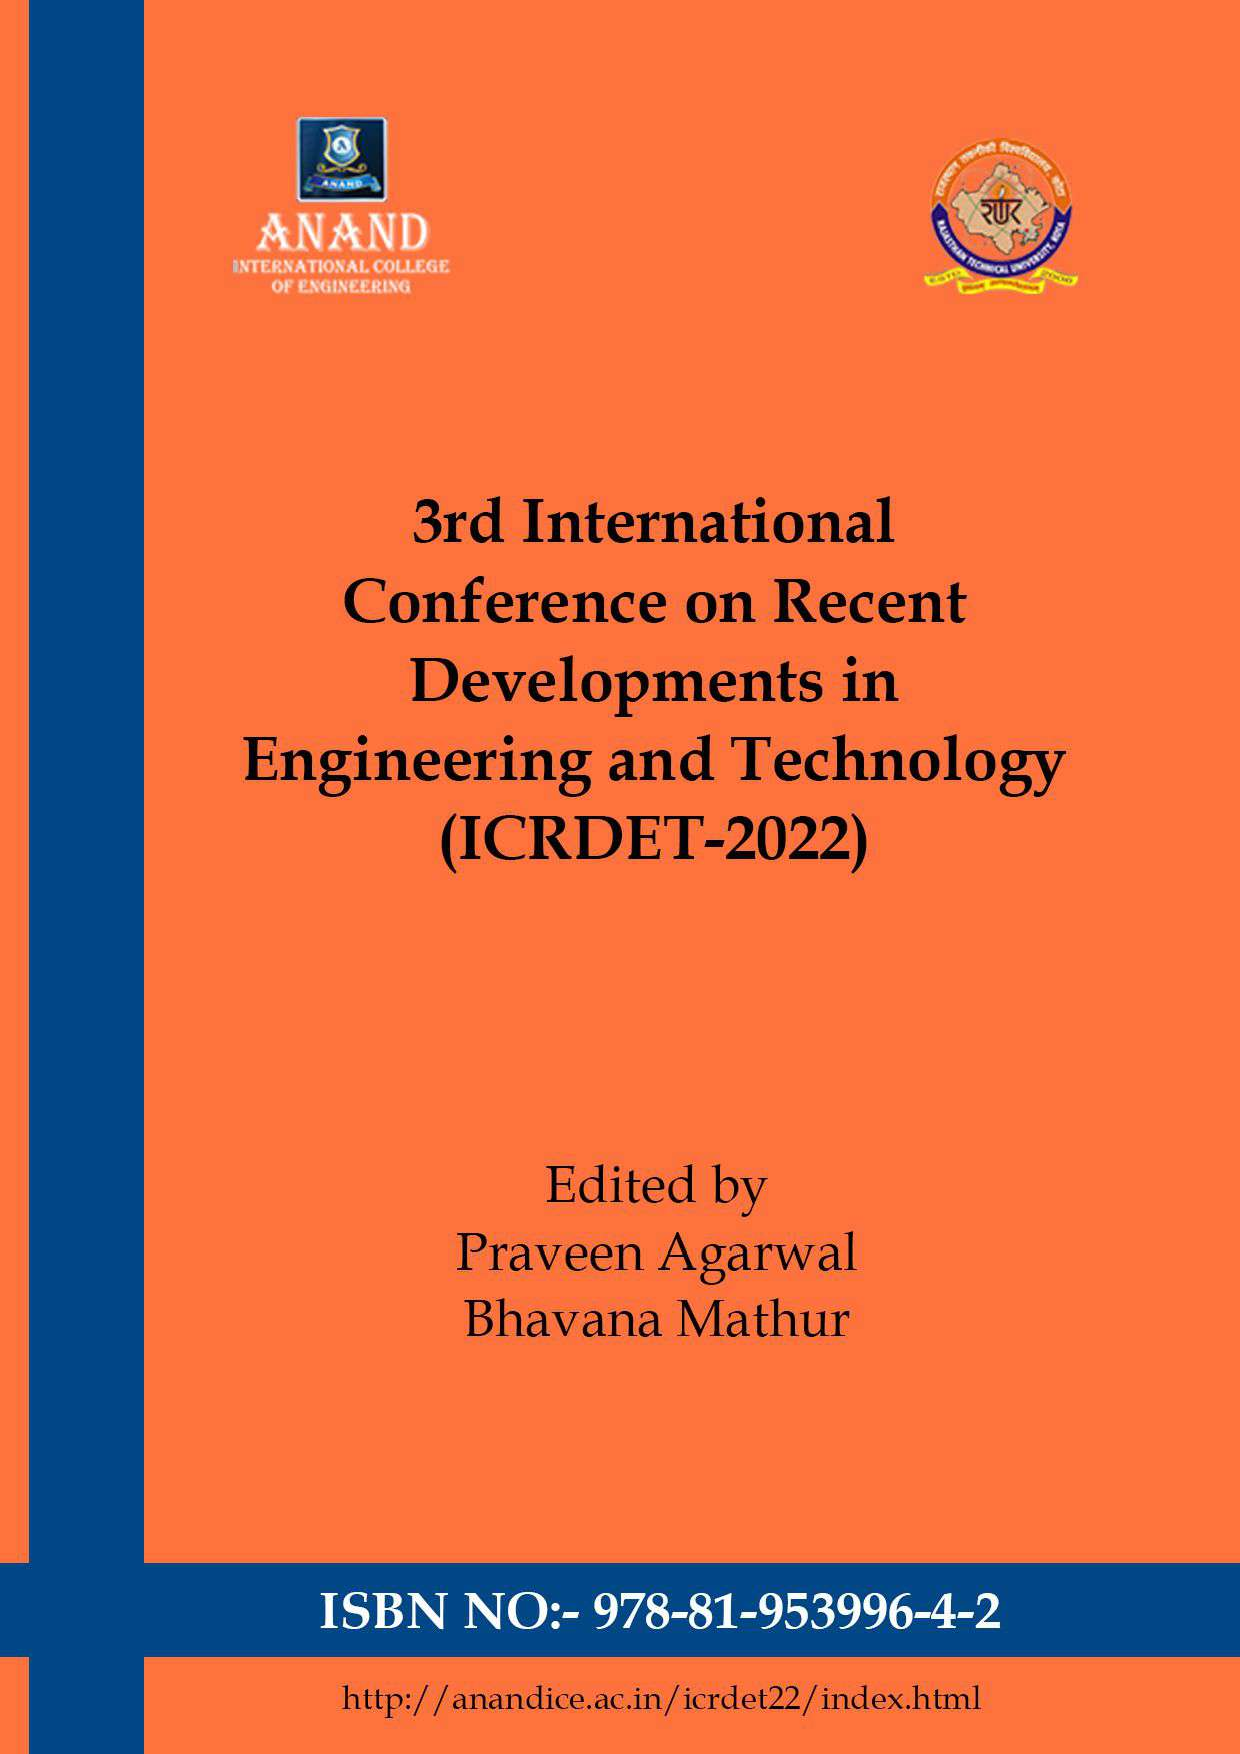
\includepdf[pages=1]{backcover}
\end{document}
%%%%%%%%%%%%%%%%%%%%%%%%%%%%%%%%%%%%%%%%%%%%%%%%%%% End of Abstract %%%%%%%%%%%%%%%%%%%%%%%%%%%%%%%%%%%%%%%%%%%%%%%%%%%%%%%%%%%%%%%%%%

%%%%%%%%%%%%%%%%%%%%%%%%%%%%%%%%%%%%%%%%%%%%%%%%%%%%%% OP-015 %%%%%%%%%%%%%%%%%%%%%%%%%%%%%%%%%%%%%%%%%%%%%%%%%%%%%%%%%%%%%%%%%%

%%%%%%%%%%%%%%%%%%%%%%%%%%%%%%%%%%%%%%%%%%%%%%%%%%% End of Abstract %%%%%%%%%%%%%%%%%%%%%%%%%%%%%%%%%%%%%%%%%%%%%%%%%%%%%%%%%%%%



%%%%%%%%%%%%%%%%%%%%%%%%%%%%%%%%%%%%%%%%%%%%%%%%%%%%%% OP-170 %%%%%%%%%%%%%%%%%%%%%%%%%%%%%%%%%%%%%%%%%%%%%%%%%%%%%%%%%%%%%%%%%%
%%%%%%%%%%%%%%%%%%%%%%%%%%%%%%%%%%%%%%%%%%%%%%%%%%% End of Abstract %%%%%%%%%%%%%%%%%%%%%%%%%%%%%%%%%%%%%%%%%%%%%%%%%%%%%%%%%%%%




%%%%%%%%%%%%%%%%%%%%%%%%%%%%%%%%%%%%%%%%%%%%%%%%%%%%%% OP-283 %%%%%%%%%%%%%%%%%%%%%%%%%%%%%%%%%%%%%%%%%%%%%%%%%%%%%%%%%%%%%%%%%%
